\documentclass{article}\usepackage{knitr}

\usepackage{setspace}
\usepackage{booktabs}
\linespread{1.25}

%% Luk_pohja.tex-tiedostosta
%% Oma sivukoko
\setlength{\textheight}{9in}
\setlength{\textwidth}{6in}
\setlength{\topmargin}{0in}
%% Tekstialueen keskitys sivulle (arvot löydetty kokeilemalla)
\setlength{\oddsidemargin}{0.4cm}
\setlength{\evensidemargin}{0.4cm}

\usepackage{bm}
\usepackage{url}
\usepackage{amsmath}
\usepackage{interval}
\usepackage{setspace}
\usepackage{multirow}
\usepackage{graphicx}
\usepackage{float}

\usepackage{hyperref}

\hypersetup{
    colorlinks=true,
    linkcolor=black,
    citecolor=black,
    filecolor=black,
    urlcolor=black
}

\graphicspath{ {./figures/} }

\usepackage[T1]{fontenc}
\usepackage[finnish, english]{babel}
\usepackage[utf8]{inputenc}

\onehalfspacing
\usepackage[natbibapa, nodoi]{apacite}
\usepackage{tcolorbox}

\usepackage{algorithm}
\usepackage[noend]{algpseudocode}





\IfFileExists{upquote.sty}{\usepackage{upquote}}{}
\begin{document}

\thispagestyle{empty}

\thispagestyle{empty}
\begin{center}
\null\vspace{3cm}
\Large
Bayesian Inference and Adaptive Estimation in General Recognition Theory\\[2cm]
\large
Joni Pääkkö\\[1cm]
\vfill
\normalsize
\end{center}
\begin{flushright}
Maisterintutkielma\\
Jyväskylän Yliopisto\\
MUTKU\\ 
Kevät 2020
\end{flushright}

\newpage

\begin{abstract}

General Recognition Theory (GRT) is a multidimensional generalization of Signal Detection Theory. It is used to model the detection of signals with multiple dimensions, e.g. auditory signals which can vary not only in their pitch but also in their timbre independently. Main focus is in if the detection of these dimensions is coupled.

Bayesian adaptive estimation has been succesfully applied to many different tasks and models in psychophysics. The main goal of this thesis is to study the application of it to GRT models. To achieve this, I will introduce a GRT models for a Yes/No and 2I-4AFC procedure that include psychometric functions to model the relationship between physical signal strengths and $d'$ explicitly. Also, methods for Bayesian estimation of these models are introduced.

The performance of the models are evaluated in simulations (N = 772) and in a small scale psychophysical experiment (N = 2).

Simulations indicate that the adaptive algorithm is more efficent on average, but offers little practical improvement over random sampling in this context. 

Data from the psychophysical experiments indicate that non-sensory factors play a big part, indicating that more work should be put into developing models/procedures that can identify between these factors. The data also suggests that the often default choice of coupling means does not necessarily capture all relevant properties of it. 

\end{abstract}

\newpage

\tableofcontents

\newpage

\setcounter{page}{1}

\newpage

%!Rnw root = ../Main.Rnw

\section{Introduction}

Perception can be thought of as being multidimensional, that is natural stimuli can be decomposed into their constituent dimensions. For example, a single tone played with a guitar could be said to consist of pitch, length and timbre, which are some of the dimensions of an auditory signal, in this case, a musical tone. Another way in which perception is multidimensional is when it is \textit{multimodal}: in many situations we combine information from different sensory modalities, for example haptic and auditory information when pressing a key on the keyboard, or visual and auditory information when watching someone's lips as they speak.

How we perceive such multidimensional signals is a fundamental psychological question: during perception, are the dimensions processed independently, or do they interfere with each other? Is the perception of auditory signals influenced by visual or other signals, and if so, in what situations? Do the physical dimensions, such as amplitude, correspond to the psychological (in this case loudness) or do we perceive them as combinations (do e.g. high pitches sound louder)?

A popular approach is the General Recognition Theory (GRT), which is a multidimensional generalization of Signal Detection Theory (SDT) (\citealp{wickens2002,ashby1986, ashby2015}). SDT is a much-studied mathematical framework describing--among other things--the detection of signals in the presence of noise. Thus, GRT offers a theoretical framework for modelling multidimensional perception. 

Most experiments employing GRT use preselected stimuli, i.e. use a paradigm called \textit{method of constant stimuli} (MOCS).  However, it is known that using methods that can adapt the stimulus values to the behaviour of the subject can make the testing more efficient (\citealp{kontsevichtyler1999}). These kinds of methods are usually simply referred to as \textit{adaptive} methods.

The main focus of this thesis is in applying Bayesian adaptive estimation to General Recognition Theory (GRT). However, this is a multifaceted problem, and it's useful to break it down into a few separate topics. I will present the reader with a brief roadmap into these topics, and where they are discussed in more detail. However, one should also be aware that all of these issues are closely interrelated.

First, the "classic" GRT models could be described as non-parametric in the sense that they don't parameterize the relationship between the signal strength and the probability of a response; response probabilities are calculated only for stimulus categories. However, in order to meaningfully implement the adaptive method, one should be able to calculate response probabilities for arbitrary stimuli. In order to achieve just this, I will be integrating psychophysical functions into the theory of GRT. This constitutes the main part of section \ref{sec:GRT} \textit{\nameref{sec:GRT}}.  

Second, when such functional relationships are implemented, the question of \textit{how} or what kind of functional relationships between stimuli and responses should be modelled becomes an issue. There are many different kinds of functions one can choose from, and many kinds of interactions that one could incorporate into the model. This issue will be touched upon in section \ref{sec:GRT} when \textit{mean shift} and \textit{variance shift} interactions are discussed, and also in the context of hierarchical models in section \ref{sec:hierarchical_models} \textit{\nameref{sec:hierarchical_models}}. Practical ramifications of this are discussed when analysing the data from the psychophysical experiments. 

Related to this, I will be criticizing the implementation of the "classic" 2X2 detection experiment in the context of auditory psychophysics and, instead, arguing for a model based on auditory discrimination. The main gist is that it is unlikely that participants wouldn't be basing their categorization decisions based on the perceived difference to the preceding stimulus.

Third, Bayesian statistical inference is different from the usual frequentist methods used when analysing GRT models. This is most apparent in how the concept of \textit{interaction} is not dependent on statistical significance, but rather the posterior probability densities for the coefficients that model interactions. This is, of course, closely related to the previous point, since the choice of the model determines how those coefficients are to be interpreted. 

Fourth, Bayesian adaptive estimation requires, as its name already implies, the calculation of prior and posterior probability densities. This is mainly a computational problem: since the aim of adaptive estimation is to select optimal stimuli in "real time", the algorithms used have to be relatively lightweight. The posterior probability densities are not analytically calculable, so approximations based on Monte Carlo methods (random sampling) are used. This issue is discussed in section ERROR.

Related to all of the above angles are multiple practical problems, such as how to maximize the function that describes the optimality of stimuli, how many random samples one should use when approximating the posterior probability densities, what kind of parameterization of the likelihood function to use, what is the most comfortable way of inputting responses for participants and so on. 

The reader should be aware that what is being evaluated here is the intersection of all the factors just mentioned, and changing any of these would change the results. This limits the generalizability of the results, which is a common problem with studies like this. The main contribution of this thesis, then, is to explore the application of Bayesian (adaptive) methods to GRT and map some of the problems associated with this.

The work is divided into three main parts: The first part describes GRT, beginning from Signal Detection Theory and gradually exposing the reader to the models used in this thesis (Section \ref{sec:GRT} \textit{\nameref{sec:GRT}}); Second part describes Bayesian statistics and the adaptive algorithm used here (Section \ref{sec:bayes} \textit{\nameref{sec:bayes}}); The final part consists of simulations and psychophysical experiments which are used to evaluate the models (Sections \ref{sec:simulations} \textit{\nameref{sec:simulations}} and ERROR).

\newpage

%!Rnw root = ../Main.Rnw

\section{General Recognition Theory}
\label{sec:GRT}

The central theoretical concept in this work is General Recognition Theory (GRT), which is essentially a generalization of Signal Detection Theory (SDT) to multiple dimensions, with a focus on modelling interactions between them. Due to this hierarchy, I will first introduce the reader to SDT, before discussing GRT.

Both SDT and GRT are discussed in the context of a \textit{discrimination task}. In such a task a single stimulus consists of two components: the \textit{reference tone} and the \textit{test tone}, as shown schematically  in Figure \ref{fig:discrtask}. If for example the dimension of interest is pitch, the reference tone would always be the same, e.g. 150 Hz, and the test tone would either be the same or higher pitch than the reference tone. The participant would then have to determine if there was a difference between the test and reference tones.

\begin{figure}[!htb]
\centering
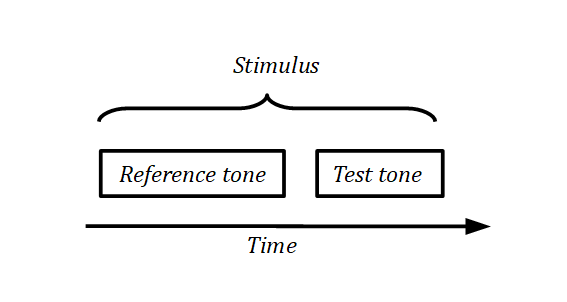
\includegraphics[scale = 0.5]{DiscriminationTask}
\caption{Schematic illustration of a stimulus in a discrimination task.}
\label{fig:discrtask}
\end{figure}

A stimulus in which the difference between reference and test tones is zero is called a \textit{noise} stimulus while one in which the difference is greater than zero is called a \textit{signal} stimulus; alternatively these can be called just noise and signal. 

\subsection{Signal Detection Theory}

Continuing the example of a  pitch discrimination task, during such experiment it is not rare to observe the participant sometimes give a negative and sometimes a positive response to the same stimulus on different presentations. The view that SDT takes is that the responses are not based directly on the physical signals, but rather some latent (unobserved) internal quantity, sometimes referred to as \textit{evidence} \citep{wickens2002} or \textit{judgments} \cite{stigler2003}. It is thought that the latent amount of evidence for e.g. the test tone being higher than the reference tone is subject to random variation, which in turn leads to variation in responses (\citet[p. 154]{kingdomprins2010}, \citet[p. 11]{wickens2002}). These random perturbations to the amount of evidence are commonly thought to arise primarily from sensory sources, but I will discuss this issue later in greater detail.

Some assumptions about the nature of the perturbations are usually made, for example that small perturbations are more common than large ones, and that the average amount of error is zero. A popular choice for modelling the distribution of the perturbations is the normal distribution with mean 0 and unknown variance. This is also the assumption that I will be making in this thesis; I will briefly return to the issue of generalizing the present approach to other distributions in the discussion section. 

By making an assumption about the distribution of the perturbations, one can calculate the predicted response probabilities for set of stimuli, and consequently make statistical inferences about the sensory processes of interest. Rest of the discussion will deal with the minutiae of these calculations. 

\subsubsection{Relationship between stimulus and $d'$}

Since the amount of evidence is assumed to be random, it can be represented as probability distributions as in Figure \ref{fig:SDT}, in which $S$ stands for physical signal level, for example the difference in frequencies between the reference and test tones. As was discussed in the previous section, normal distribution is used to model the distribution of evidence. 

If the subject is presented with a noise stimulus (one in which $S = 0$), the amount of evidence on any single trial is assumed to be a random sample from the zero-centred distribution in Figure \ref{fig:SDT}; in the context of the pitch discrimination task this would correspond with stimulus in which the test and reference pitches are identical. As $S$ is increased, the distribution from which the evidence is assumed to be sampled from shifts rightward, farther from zero, as is shown for $S = 2$ and $S = 4$.

\begin{figure}[!htb]
\begin{center}
\begin{knitrout}
\definecolor{shadecolor}{rgb}{0.969, 0.969, 0.969}\color{fgcolor}
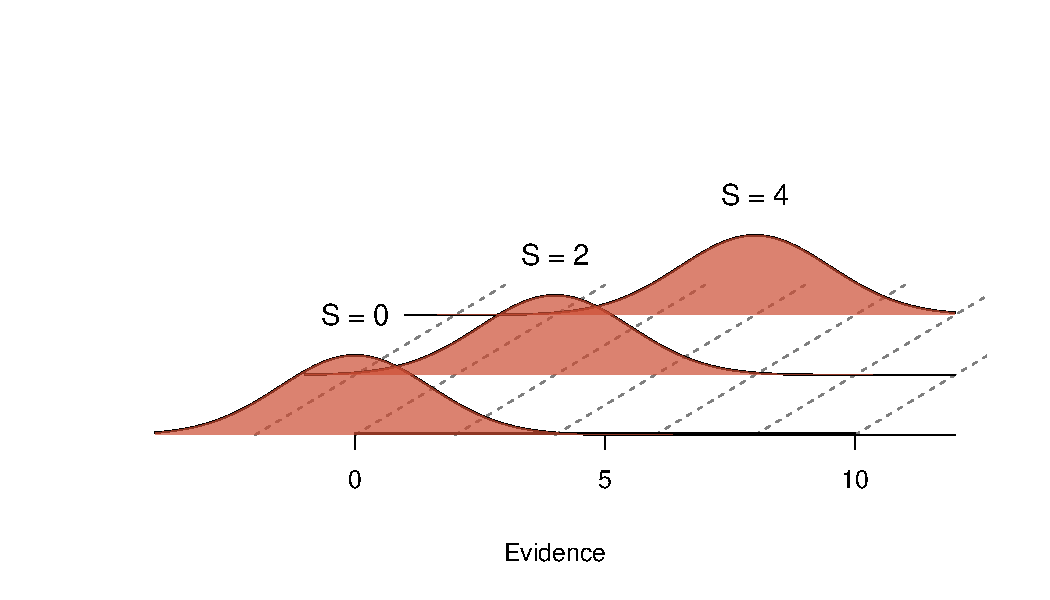
\includegraphics[width=\maxwidth]{figure/unnamed-chunk-2-1} 

\end{knitrout}
\end{center}
\caption{Evidence, according to SDT, is a random  variable. It can be assumed to be normally distributed, with monotonically increasing $\mu$ as a function of signal strength, $S$, and constant variance, $\sigma$.}
\label{fig:SDT}
\end{figure}

Signal level divided by the standard deviation of evidence is called $d'$, usually interpreted as \textit{discriminability} or \textit{signal-to-noise ratio}. Standardized in this way, the standard deviation of evidence is always one. 

Relationship between $d'$ and $S$ is not necessarily linear. Theoretically this kind of non-linearity could  arise e.g. from changes in the variance of the evidence distribution. However, the non-linearity is often interpreted as being the result of non-linearity in signal transduction, i.e. the change of physical signal into internal.\footnote{Familiar example of non-linear transduction is how pitch is experienced in large scale: in order to move one octave up on the psychological scale of pitch, one has to move increasingly fast on the physical frequency. ERROR SOURCES.}

The functional relationship between physical signal strength and $d'$ has been quantified in many different ways in the psychophysical literature (for a selection, see \citet[Appendix A]{lesmes2015}). The functional form used here is based on the widely used \textit{power law} model of signal transduction (see e.g. \citet{kontsevichtyler1999, dai2011, lesmes2015}):

\begin{equation}
d' = (\frac{S}{\sigma})^\beta
\label{eq:dprimefunc}
\end{equation}

Here $S$ is again the physical signal strength, $\sigma$ corresponds to the standard deviation of evidence and $\beta$ models non-linearity between signal level and signal-to-noise ratio. Note that often $\alpha$ is used for the standard deviation of evidence (e.g. in \cite{dai2011, kontsevichtyler1999}), but since this parameter indeed is directly related to the standard deviation of the evidence distribution, I feel $\sigma$ is more appropriate. 

The effects of changing these parameters are shown in Figure \ref{fig:dprimefunc}. The smaller $\sigma$ is, the faster $d'$ increases. $\beta$ parameter affects the linearity of the function: when $\beta < 1$ the function increases faster than the linear case before the point at which $d' = 1$ and slower after that; the opposite happens when $\beta > 1$. 

\begin{figure}[!htb]
\begin{center}
\begin{knitrout}
\definecolor{shadecolor}{rgb}{0.969, 0.969, 0.969}\color{fgcolor}
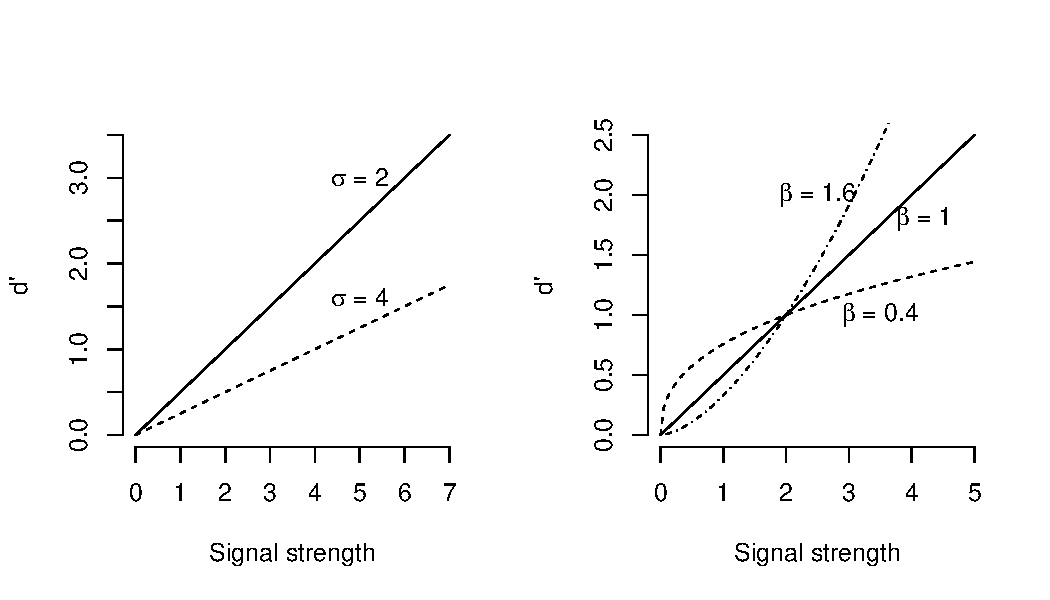
\includegraphics[width=\maxwidth]{figure/unnamed-chunk-3-1} 

\end{knitrout}
\end{center}
\caption{ The effect of $\sigma$ and $\beta$ parameters on the $d'$ function. Left panel shows the effect of changing $\sigma$ parameter while keeping $\beta$ constant and the right panel shows the effect of changing $\beta$ parameter while keeping $\sigma$ constant ($\sigma = 2$).}
\label{fig:dprimefunc}
\end{figure}

\subsubsection{Modelling responses: relationship between $d'$ and response}

The preceding discussion about relating $S$-values to $d'$-values is just one half of SDT, there has to be a way of relating the $d'$-values to responses, $R$. Usually categorical decisions are required from the participant. I will be considering two different tasks, a Yes/No task and a 2-interval 2-alternative forced choice task (2I-2AFC). These are shown schematically in Figure \ref{fig:YesNoAfc}.

\begin{figure}[!htb]
\centering
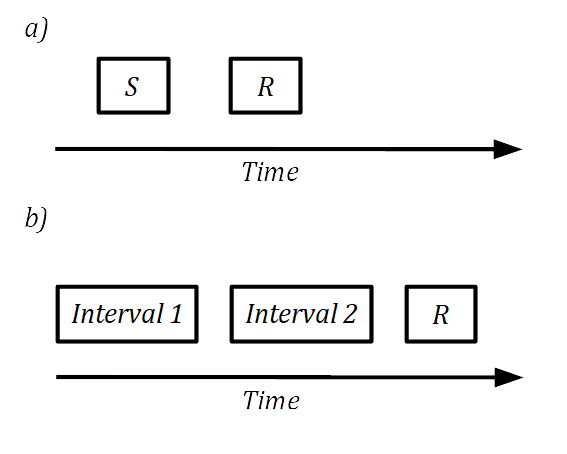
\includegraphics[scale = 0.5]{YesNoAfc}
\caption{Schematic representations of the Yes/No (panel a) and 2-interval forced choice (panel b) tasks. \textit{S = } signal, \textit{R =} response.}
\label{fig:YesNoAfc}
\end{figure}

In the Yes/No task (panel \textit{a} of Figure \ref{fig:YesNoAfc}) the participant's task is to indicate if they detected the signal. The name of the task is quite literal as the participants provide \textit{Yes} and \textit{No} answers. As shown in the figure, the participant is first presented with the stimulus, and they are then expected to give their answer.

In contrast to this, in the 2I-2AFC task the participant is presented with two \textit{observation intervals}, interval referring here to a temporal interval as can be seen from panel \textit{b} of Figure \ref{fig:YesNoAfc}. During each interval the participant is presented with a stimulus, one containing only noise and the other containing the signal. The participant's task is then to indicate which interval they thought contained the signal. Again, the name is quite literal: the participant is presented with two intervals and they have to choose their response among two alternatives.

\paragraph{Responses in the Yes/No task}

Decisional processing is modelled by assuming that the participant has an internal criterion for the evidence. When evidence is below this criterion the participant will respond negatively and when evidence exceeds the criterion they will respond  positively.

When the participant is presented with a signal stimulus, positive responses are called \textit{hits}; when they  are presented with a noise stimulus, positive responses are called \textit{false alarms}. \citep{wickens2002, kingdomprins2010}. 

Criterion is represented by the red dashed vertical lines in Figure \ref{fig:yesno}. As signal level increases, and as a consequence $d'$, the evidence distribution shifts to the right. Since the criterion is fixed, larger portion of the evidence distribution falls to the right of the criterion, indicating higher probability of a positive response.

\begin{figure}[!htb]
\centering
\begin{knitrout}
\definecolor{shadecolor}{rgb}{0.969, 0.969, 0.969}\color{fgcolor}
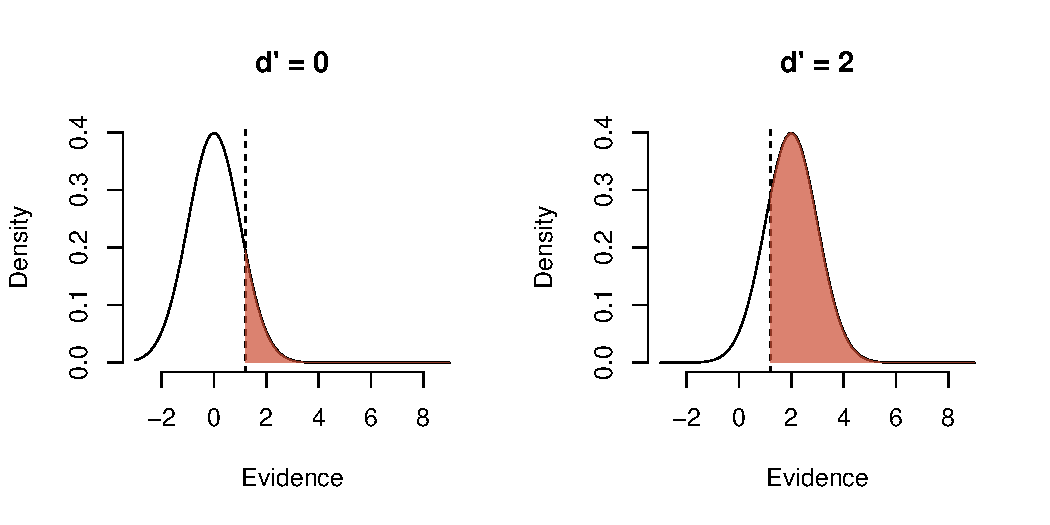
\includegraphics[width=\maxwidth]{figure/unnamed-chunk-4-1} 

\end{knitrout}
\caption{Binary decisions in the YesNo-paradigm. The distribution of evidence is divided into response regions.}
\label{fig:yesno}
\end{figure}

The probability of evidence exceeding the decisional criterion on any trial can be found by finding the area (shaded part in Figure \ref{fig:yesno}) under the normal distribution upwards from the criterion (see \citet{wickens2002, kingdomprins2010}):

\begin{equation}
\label{eq:SDTintegral}
P(R = 1) = \int_{c}^{\infty} N(d', 1)
\end{equation}

where $d'$ is the signal-to-noise ratio as calculated in equation \ref{eq:dprimefunc} and $c$, the lower bound of the integral, is the criterion. 

The integral in this equation is usually written in terms of the cumulative standard normal distribution function, $\phi$. The resulting function, denoted with the Greek letter $\psi$, is called the \textit{psychometric function}. \cite[Chapter 4]{kingdomprins2010}

Usually only the positive response is considered, since the probability of a negative response is simply the complement of it, but it is more principled to show the probabilities for both the positive and negative responses. 

\begin{align*}
\begin{split}
\psi(S; \Theta)_{\text{Yes}} &= \phi(-c + d') \\
\psi(S; \Theta)_{\text{No}} &=  1 - \phi(-c + d')
\end{split}
\end{align*}

Here $\Theta$ is a vector containing the parameters of the psychometric function, and $S$ the physical signal level.

Since sensory and decisional processes are separate in the model, keeping the parameters that model sensory processing constant while varying the criterion will result in different predicted proportions of hits and false alarms. That is to say that the perceptual processing capabilities can be exactly the same for two participants, but the observed amounts of hits and false alarms can be different, if one participant has a more lax criterion. This is shown in the left panel of Figure \ref{fig:critchange}.

It is important to notice how hits and false alarms are coupled. If the participant wants to avoid false alarms, they will have to adopt a stricter criterion for the evidence, and  as a consequence they  will inevitably also make less hits. This is because the aim of SDT is to model situation in which there is a non-zero probability of confusing signal with noise. 

The coupling between hits and false alarms is demonstrated in the form the a \textit{receiver operating characteristic} (ROC) curve \cite[161]{kingdomprins2010} in the right panel of Figure \ref{fig:critchange}. When the participant adopts stricter criterion, they move left on the ROC curve. When the signal is stronger ($d'$-value is higher), the participant is able to hit more hits. 

Note that if the participant aims to avoid false alarms altogether, they will have to adopt a criterion that, theoretically, would also result in zero hits; the criterion has to be relaxed a bit in order for the participant to perform in the task in any meaningful way, resulting in some false alarms and hits, as just discussed. Generally, the participant is free to "set their own criterion", however it is possible to calculate the optimal value of the decisional criterion. 

\begin{figure}[!htb]
\begin{center}
\begin{knitrout}
\definecolor{shadecolor}{rgb}{0.969, 0.969, 0.969}\color{fgcolor}
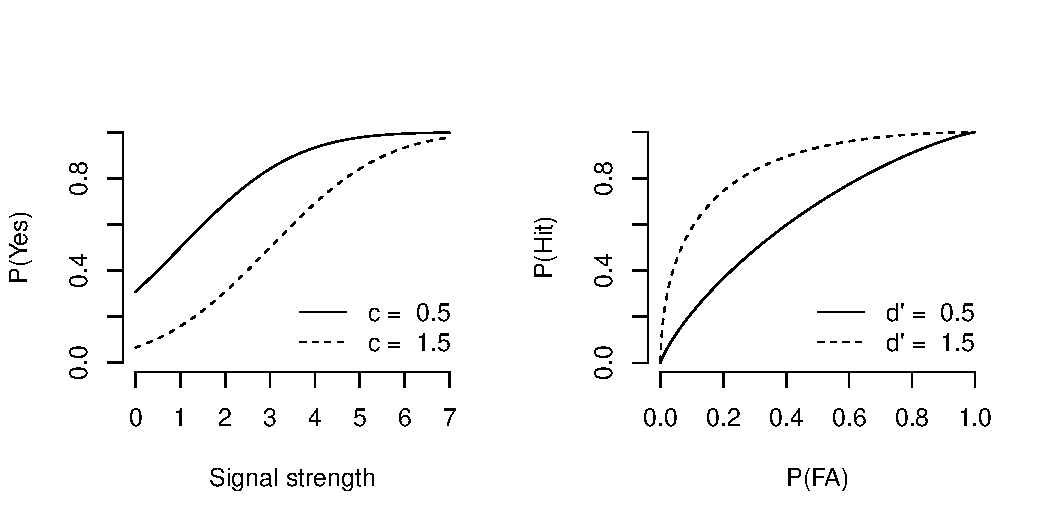
\includegraphics[width=\maxwidth]{figure/unnamed-chunk-5-1} 

\end{knitrout}
\end{center}
\caption{ Decisional processing in Signal Detection Theory. Left panel: The effect of differing criteria on the predicted amounts of false alarms and hits while the parameters describing the sensory processing are kept constant. \textit{Higher} criterion value implies stricter criterion--that the participant is less willing to respond \textit{yes}--while a \textit{lower} value implies more lax criterion. Right panel: Receiver operating characteristic (ROC) curve for two fixed $d'$-values, showing that the proportions of hits and false alarms are coupled.}
\label{fig:critchange}
\end{figure}

\paragraph{Responses in the 2I-2AFC task}

Since the participant is presented with two stimuli in the 2I-2AFC task, theoretically the participant is comparing two random numbers, one representing strength  of evidence in the first interval and the other representing strength of evidence in the second interval. From which ever interval the larger of these two was from gets picked as the \textit{signal} interval by the participant.

As a consequence the signal-to-noise ratio is decreased compared to the Yes/No task. Intuitively this can be understood by noticing that if one compares two things, both of which contain uncertainty, the individual uncertainties add up. Mathematically speaking, the participant can be thought of basing their decision on decision variable (here $dv$) that is the difference of the two random variables:

\begin{equation}
dv = [N(d', 1) - N(0, 1)] I
\end{equation}

Here $I$ is an indicator variable which  is $-1$ when the signal is in the first interval and $1$ when the signal is in the second interval. Consequently the decision rule is to respond \textit{Interval 1} when the decision variable $dv$ is negative and \textit{Interval 2} when it's positive. 

It is usually more practical, however, to think about the responses in terms of hits and false alarms, similar to the Yes/No task. This makes it possible to drop the the indicator variable from the equation, since we are only interested in the difference between the signal and noise distributions. This basic structure of the 2AFC model is demonstrated in Figure \ref{fig:2AFC}. 

\begin{figure}[!htb]
\centering
\begin{knitrout}
\definecolor{shadecolor}{rgb}{0.969, 0.969, 0.969}\color{fgcolor}
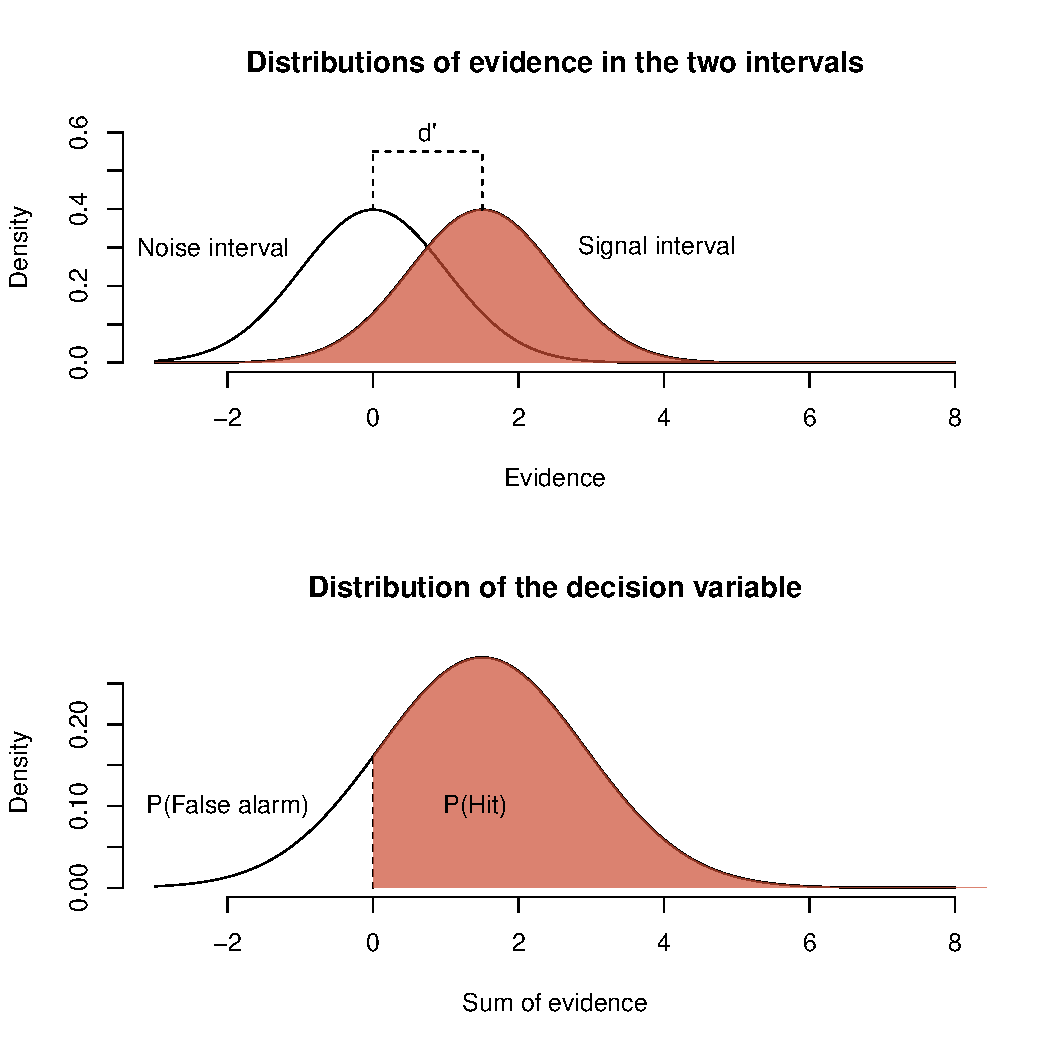
\includegraphics[width=\maxwidth]{figure/unnamed-chunk-6-1} 

\end{knitrout}
\caption{How responses are generated in the forced choice task. In the upper panel, the shaded distribution shows distribution of evidence from the signal interval while the non-shaded distribution shows evidence from the noise interval. The lower panel shows the distribution of the decision variable. }
\label{fig:2AFC}
\end{figure}

In the upper panel the zero-centred distribution represents evidence from the noise-only interval while the distribution centred on 1.5 represents evidence from the signal interval. Irregardless of whether the signal is in the first or second interval, the signal interval will be shifted $d'$ amount. Since the probability of making the correct decision is the proportion of the decision variable distribution that exceeds 0, shifting the signal distribution to the right will increase this probability--as one would expect.

What is important to note is that the decision variable is the difference of two normally distributed random variables, both with standard  deviation of one, since they represent the standardized quantity $d'$. It follows from the additivity of variances ERROR SOURCE, and from the fact that standard deviation is the square root of variance ERROR SOURCE, that the standard deviation of the decision variable is $\sqrt{2}$. It follows then that the $d'$ values in the psychometric function have to be divided by $\sqrt{2}$:

\begin{align*}
\begin{split}
\psi(S; \Theta)_{\text{Hit}} &= \phi(\frac{d'}{\sqrt{2}}) \\
\psi(S; \Theta)_{\text{False alarm}} &=  1 - \phi(\frac{d'}{\sqrt{2}})
\end{split}
\end{align*}

The term $c$ is dropped since it is assumed that, on average, the observer isn't biased towards either of the intervals. This assumption can be relaxed by including the term $c$ in the model, but in this work this possibility is not pursued any further. Some bias is probably not detrimental: any such bias would presumably be most noticeable when the signal level is low, and in these cases performance is already close to chance. 


%!Rnw root = ../Main.Rnw

\subsection{Signal Detection Theory in two dimensions}

So far I have covered the case in which the participant has to make a single decision, e.g. if the pitch of the stimulus changed. In the two-dimensional case the participant has to observe two things at once. For example did the pitch change \textit{and} did the timbre change. The question of primary interest is if there are any \textit{interactions} between the dimensions: does changing timbre also change response probabilities to pitch changes.

A widely used theoretical framework for generalizing SDT into multiple dimensions is the General Recognition Theory. As in SDT, also in GRT randomness in the responses is thought to arise from the evidence having a probabilistic nature \citep{ashby1986, ashby2015, kadlec1992}. 

In the two-dimensional case also the evidence distribution is two dimensional. Following the assumption made earlier that evidence is distributed normally, it is possible to represent evidence in two dimensions by a bivariate normal distribution. This is demonstrated in Figure \ref{fig:2dimnorm}. Left panel shows a projection of the 3-dimensional shape of the bivariate density; right panel shows the same distribution from above, as a contour.  

\begin{figure}
\centering
\begin{knitrout}
\definecolor{shadecolor}{rgb}{0.969, 0.969, 0.969}\color{fgcolor}
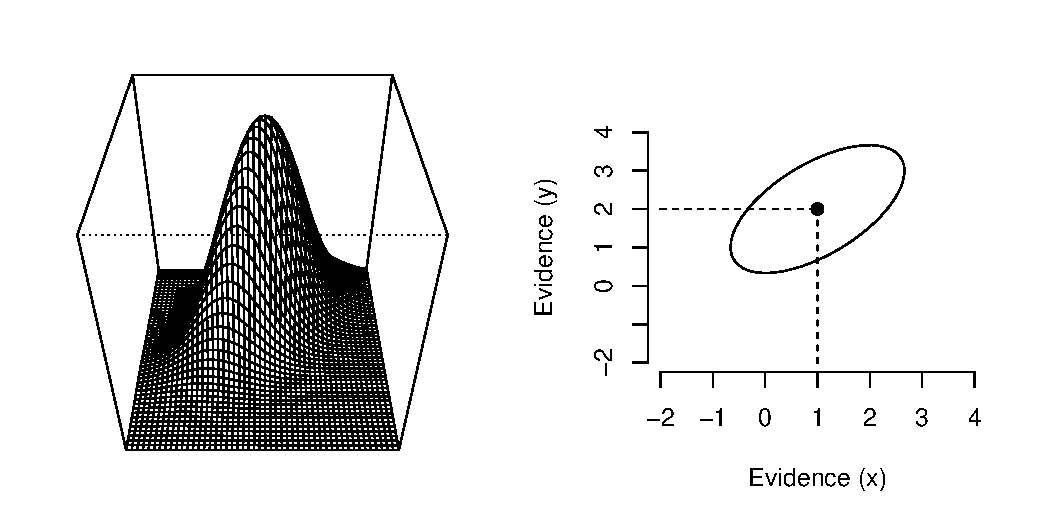
\includegraphics[width=\maxwidth]{figure/unnamed-chunk-7-1} 

\end{knitrout}
\caption{Two projections of a two-dimensional normal distribution with the parameters $\mu = [1.0, 2.0]^T$, $\rho = 0.6$}. 
\label{fig:2dimnorm}
\end{figure}

\subsubsection{Calculation of $d'$ in two dimensions}

In the one dimensional case $d'$ value tells the location, i.e. $\mu$, of the evidence distribution on the evidence axis. Situation in two dimensions is similar to this, however, now $\mu$ becomes a vector with two possible values corresponding to the location of the evidence distribution on the two dimensions: $\bm{\mu} = [\mu_x, \mu_y]^T$. Here $\mu_x$ could correspond to evidence about pitch change and $\mu_y$ to evidence about timbre change. In Figure \ref{fig:2dimnorm} $\mu_x$ is represented by the vertical dashed line, while $\mu_y$ is represented by the horizontal dashed line.\footnote{Note that the vector $\bm{mu}$--and all vectors after his--is transposed (the $T$ in the superscript) since it is customary to define these as column vectors.}

Since there are two $d'$ and $\mu$ parameters, also the parameters of the psychometric function (cf. chapter on unidimensional SDT), signals and responses become vectors: $\bm{\sigma} = [\sigma_x, \sigma_y]^T$, $\bm{\beta} = [\beta_x, \beta_y]^T$, $\bm{S} = [S_x, S_y]^T$ and $\bm{R} = [R_x, R_y]^T$. In addition to this, since interactions between the dimensions are of interest, the parameter $\kappa$ (for \textit{coupling}) is added to the equation: $\bm{\kappa} = [\kappa_x, \kappa_y]^T$. In practice, it is useful to think about this as two coupled $d'$ functions, which will be defined in the next section.

\subsubsection{Coupling between the functions}

I will be considering two different types of coupling between the $d'$ functions. The first type is coupling between the means of the evidence distributions, the other kind is coupling between the variances of the evidence distributions. 

\begin{align}
\label{eq:twodimdprime}
\begin{split}
d'_x &= (\frac{S_x}{\sigma_x})^{\beta_x} + \kappa_x^{\mu} S_y \\
d'_y &= (\frac{S_y}{\sigma_y})^{\beta_y} + \kappa_y^{\mu} S_x
\end{split}
\end{align}

Through the parameter $\kappa_i^{mu}$ any non-zero signal on the other dimension is able to influence the $d'$ value of the other dimension, as demonstrated in the left panel of Figure \ref{fig:GRTinteractions}. This is usually referred to as mean-shift integrality; other term for this is \textit{sensory interference} ERROR SOURCE. The term integrality refers to classification of dimensions into that of \textit{separable} and \textit{integral} (ERROR SOURCES); this sort of binary classification will be contested later.

The other possibility is that the $\sigma$ terms are coupled:

\begin{align}
\label{eq:varshift}
\begin{split}
\sigma_x &= exp(log\sigma_x + \kappa_x^{\sigma} S_y) \\
\sigma_y &= exp(log\sigma_y + \kappa_y^{\sigma} S_x)
\end{split}
\end{align}

Note that in the \textit{Yes/No} model also the criteria have to be divided by $\sigma$--this will be discussed at the end of the section on the \textit{Yes/No} model.

\paragraph{Within stimuli interference}

It is also possible that the evidence is correlated between the dimensions: see the right panel of Figure \ref{fig:GRTinteractions}. This is sometimes also referred to as \textit{perceptual interference} or \textit{correlated noise}. Correlated evidence is not included in the $d'$ functions; it affects only the response probabilities and will be discussed in conjunction with the psychometric functions. 

\begin{figure}
\begin{center}
\begin{knitrout}
\definecolor{shadecolor}{rgb}{0.969, 0.969, 0.969}\color{fgcolor}
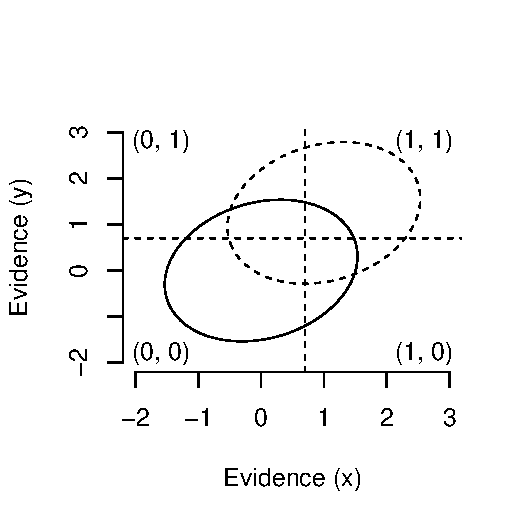
\includegraphics[width=\maxwidth]{figure/unnamed-chunk-8-1} 

\end{knitrout}
\end{center}
\caption{The two kinds of interactions in the model. The contours depict bivariate normal distributions. Dashed lines indicate the shape and location of the distribution in the absence of interaction; the solid lines depict them in the case that interaction is present. Left panel demonstrates a shift in the mean of the latent distribution. Right panel demonstrates correlated noise between the dimensions.}
\label{fig:GRTinteractions}
\end{figure}

\subsubsection{Modelling responses in two dimensions}
\label{sec:modelling_responses}

Whereas in SDT the participant is usually required to make a single decision on a single axis, in GRT the participant is required to make one decision per axis; in the two-dimensional case two decisions: did the signal level change on $x$ axis and did the signal level change on $y$ axis (a similar approach has been used also by \cite{wickens1992}). 

\paragraph{Yes/No task in two dimensions}

Figure \ref{fig:GRTsimple} shows discrimination in two dimensions analogously to how it was shown from SDT Figure \ref{fig:SDT}. The contours represent the bivariate normal distributions, as seen from above. Because the signal is two-dimensional, the participant has to hold two decisional boundaries, here represented by the dashed lines that divide the internal scale into four response regions. Numbers in each corner correspond to the different response categories: 0 indicating a negative response on that dimension and 1 a positive response. In this case the most probable response is $[1,1]$, a positive response on both dimensions.

\begin{figure}
\begin{center}
\begin{knitrout}
\definecolor{shadecolor}{rgb}{0.969, 0.969, 0.969}\color{fgcolor}
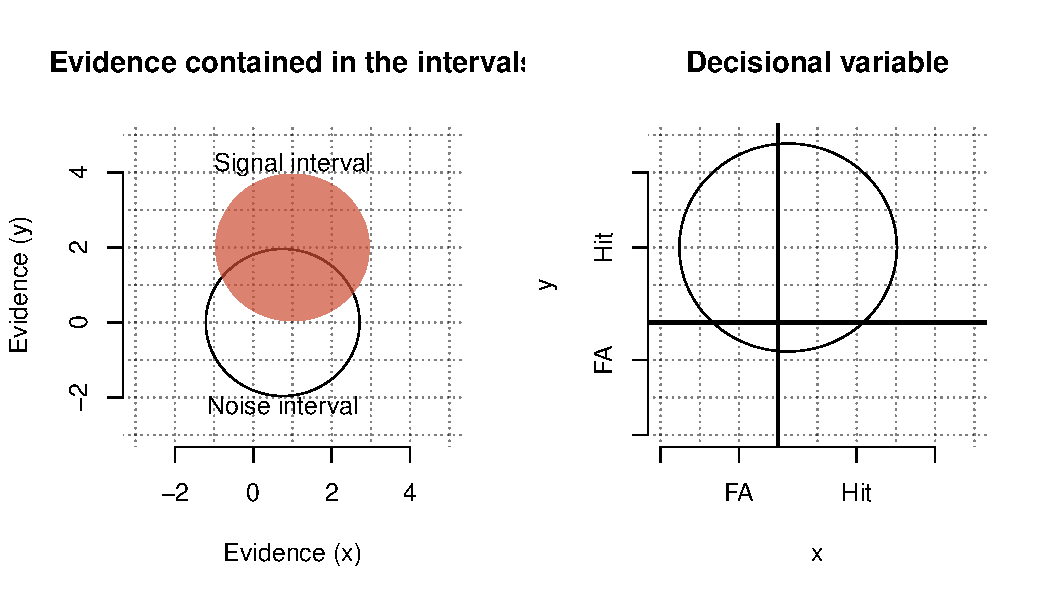
\includegraphics[width=\maxwidth]{figure/unnamed-chunk-9-1} 

\end{knitrout}
\end{center}
\caption{Discrimination in two dimensions.}
\label{fig:GRTsimple}
\end{figure}

Again, similar to unidimensional SDT, the response probabilities are found by integrating over the evidence distribution, split into response regions by the decisional boundaries (c.f. Figure \ref{fig:GRTsimple}). For example the probability of observing a positive response on both dimensions is found by  integrating the two-dimensional normal distribution from the response criteria to positive infinity. Whereas in the unidimensional case two psychometric functions were needed to model the binary responses, here four are needed, for each of the response possibilities:

\begin{align}
\begin{split}
\label{eq:probs}
\psi(\bm{S}; \theta)_{(0, 0)}  = \int_{-\infty}^{C_x} \int_{-\infty}^{C_y} N(\bm{\mu}, \bm{\Sigma})
\\
\psi(\bm{S}; \theta)_{(1, 0)}  = \int_{C_x}^{\infty} \int_{-\infty}^{C_y} N(\bm{\mu}, \bm{\Sigma})
\\
\psi(\bm{S}; \theta)_{(0, 1)}  = \int_{-\infty}^{C_x} \int_{C_y}^{\infty} N(\bm{\mu}, \bm{\Sigma})
\\
\psi(\bm{S}; \theta)_{(1, 1)}  = \int_{C_x}^{\infty} \int_{C_y}^{\infty} N(\bm{\mu}, \bm{\Sigma})
\end{split}
\end{align}

Here $\bm{S}$ is a vector containing the physical signal levels on the individual dimensions, $\bm{\mu}$ corresponds to the vector of $d'$-values. $\bm{\Sigma}$ is the correlation matrix, in which correlated evidence--see right panel of Figure \ref{fig:GRTinteractions}--is modelled by treating the correlation coefficient as a free parameter:

$$
\begin{bmatrix}
1 & \rho \\
\rho & 1
\end{bmatrix}
$$

Again, the psychometric functions are most practically thought about in terms of the bivariate standard normal cumulative distribution function, $\phi_2(u_x, u_y, \rho)$ (\cite{boys1989, pan2017}). First one has to find $u_x$ and $u_y$ (the first two inputs to $\phi_2$) which stand for the upper integration limits:

\begin{align*}
\begin{split}
u_x &= -c_x + d'_x \\
u_y &= -c_y + d'_y
\end{split}
\end{align*}

Then, if responses are coded with $-1$ and $1$, inputs for the $\phi_2$ function are:

\begin{align*}
\begin{split}
\psi_2(\bm{S}; \theta)_{\text{(-1, -1)}} &= \phi_2(-1 u_x, -1 u_y, \rho [-1 * -1]) \\
\psi_2(\bm{S}; \theta)_{\text{(1, -1)}}  &= \phi_2(\phantom{-}1 u_x, -1 u_y, \rho [\phantom{-}1 * -1]) \\
\psi_2(\bm{S}; \theta)_{\text{(-1, 1)}}  &= \phi_2(-1 u_x, \phantom{-}1 u_y, \rho [-1 * \phantom{-}1]) \\
\psi_2(\bm{S}; \theta)_{\text{(1, 1)}}   &= \phi_2(\phantom{-}1 u_x, \phantom{-}1 u_y, \rho [\phantom{-}1 * \phantom{-}1]) 
\end{split}
\end{align*}

This process can be defined generally with the equation:

\begin{equation}
\psi_2(\bm{S}; \theta)_{\bm{R}} = \phi_2([-c_x + d'_x]r_x, [-c_y + d'_y] r_y, \rho [r_x r_y])
\label{eq:generalPfun}
\end{equation}

in which the $\bm{R} = [r_x r_y]$. All of the Stan \citep{stan2019} programs in appendix A assume that responses are coded in this way.

In the case of variance shift also the criterion has to be also divided by the standard deviation. This is intuitively clear from the observation that as the variance of the evidence distribution becomes larger, the parts of the evidence distribution falling into the response regions become increasingly equal. In other words response probabilities get closer to 0.25, and a larger denominator for the term $c$ will achieve just this:

\begin{equation}
\psi_2(\bm{S}; \theta)_{\bm{R}} = \phi_2([-\frac{c_x}{\sigma_x} + d'_x]r_x, [-\frac{c_y}{\sigma_y} + d'_y] r_y, \rho [r_x r_y])
\label{eq:generalPfun}
\end{equation}  

The term $\sigma$ is also affected  and is defined in equation \ref{eq:varshift}.

\paragraph{2I-4AFC}

In the SDT section 2I-2AFC task was discussed. Here it is expanded to a 2I-4AFC task. There are still two temporal intervals, as was shown in the schematic in Figure \ref{fig:YesNoAfc}, but now the participant has four response alternatives, since either signal could be in either interval. What has to be taken into account is that there can be interactions, which means that the mean of the noise distribution on either dimension can be non-zero. 

Similar to Figure \ref{fig:2AFC}, Figure \ref{fig:2I4AFC} shows the distributions of evidence from the two intervals. Note that each of the signals could be in either of the intervals, so there are four possible arrangements for the signals, but similar to the case in 2I-2AFC it is not important in which intervals the signals are concretely, what is important is the difference between the signal and noise distributions. 

It is assumed in Figure \ref{fig:2I4AFC} that $\kappa_x$ parameter is non-zero, which means that signal on $y$-dimension is able to increase the $d'$-value on the $x$-dimension. This can be seen from the fact that in the left panel the mean of the noise distribution on the $x$-axis is slightly greater than zero. This shrinks the difference between the signal and noise distributions on that dimension.

As before, the participant is thought to base their decision on a decision variable that represents the difference of evidence in the intervals. As a consequence the $d'$ values on both dimensions have to be divided by $\sqrt{2}$ (cf. section on 2I-2AFC). The distribution of the decisional variable can be seen in the right panel of Figure \ref{fig:2I4AFC}. The thick black lines mark boundaries between \textit{hits} and \textit{false alarms}. The participant, in this particular scenario, is very likely to score a \textit{hit} on the $y$-axis, but on $x$-axis they are almost as likely to pick the wrong interval as the correct; the most likely response pairs being (FA, Hit) and (Hit, Hit).

\begin{figure}
\centering
\begin{knitrout}
\definecolor{shadecolor}{rgb}{0.969, 0.969, 0.969}\color{fgcolor}
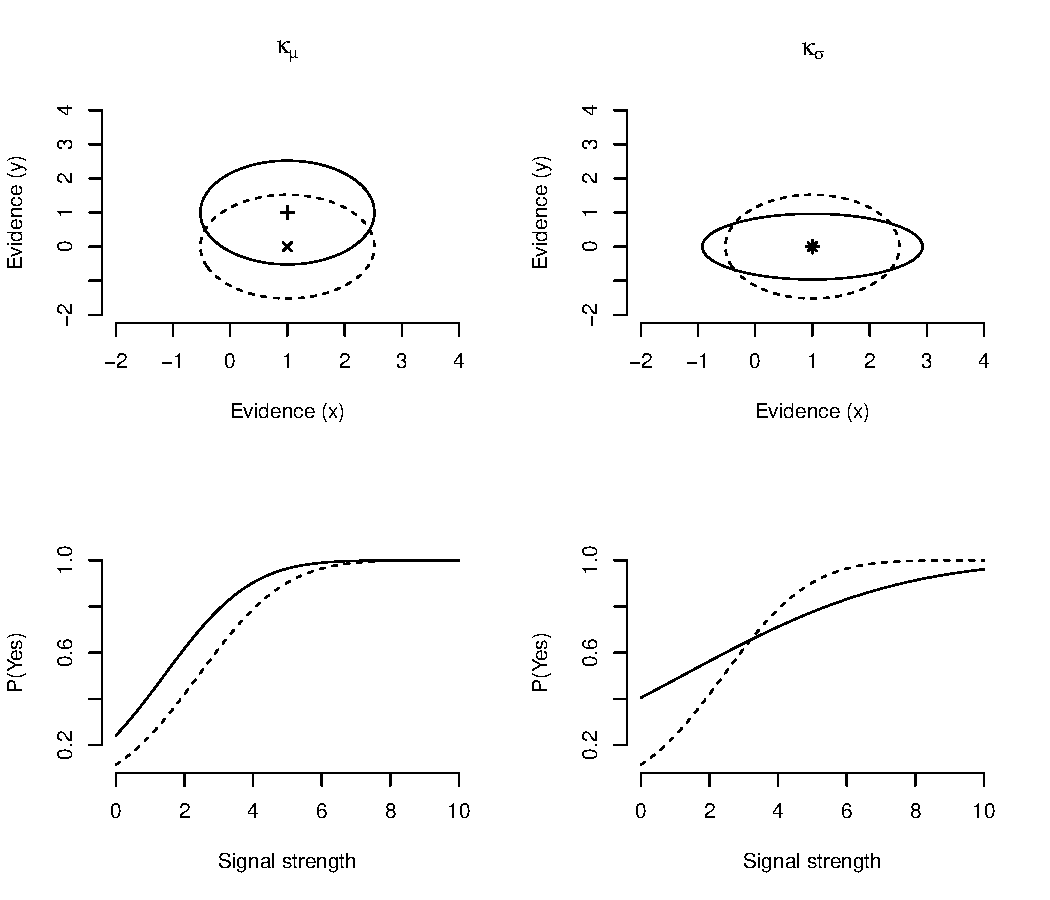
\includegraphics[width=\maxwidth]{figure/unnamed-chunk-10-1} 

\end{knitrout}
\caption{}
\label{fig:2I4AFC}
\end{figure}

As in the Yes/No task, responses can be coded with -1 and 1. Here, \textit{false alarms} are coded with -1 and \textit{hits} with 1.  The psychometric functions is then simply

\begin{equation}
\psi_2(\bm{S}; \theta)_{\bm{R}} = \phi_2(\frac{d'_x}{\sqrt{2}}r_x, \frac{d'_y}{\sqrt{2}} r_y, \rho [r_x r_y])
\label{eq:generalPfun2}
\end{equation}

\paragraph{Comparison of the Yes/No and 2I-4AFC tasks}

The main difference between the Yes/No and 2I-4AFC tasks is what the participant bases their decision on. In the Yes/No task the decision is based directly on the appearance of the stimulus. As was already discussed, this means that the performance of the observer cannot be decoupled from their decisional criterion. This adds one more parameter to be estimated from the data. 

In the 2I-4AFC task the decision is removed one step from the signal compared to the Yes/No task. This means that it is not necessary for the participant to adopt a criterion relating the strength of evidence to a response. Also, since the participants are choosing an interval, it is usually thought that this kind of task is less susceptible to bias.

Since on each trial two stimuli have to be presented in the 2I-4AFC task, it is somewhat slower to administer. However, if, in the Yes/No task, the observer knows that some non-zero signal is present on each trial, nothing prevents them from answering \textit{yes} on each trial--they will always be correct, and seemingly able to detect the faintest of signals. To counter this, some amount of \textit{catch} trials are usually included. These are trials during which the signal level is zero. During these trials no information about the sensory processing--the parameters $\alpha$ and $\beta$--is accumulated. So even though individual trials are faster to complete, there has to be more of them. 

The issue of catch trials is exacerbated in the multidimensional case. This is because in the one-dimensional the issue is simple solved by including some noise stimuli as catch trials in the experimental run, resulting in two kinds of stimuli being presented: noise and signal stimuli. In the two-dimensional case there has to be three kinds of catch trials: noise only stimulus on either of the dimensions or both. Otherwise if the participant became aware of e.g. that the adaptive procedure only rarely selects a stimulus in which there's a noise stimulus on either dimension--i.e. [0,S] or [S,0] --, they might become biased towards choosing the responses [0, 0] and [1,1]. The linear decision bounds used in this work are not able to model this kind of response bias; an issue which will be discussed later. 

Then, on theoretical grounds, the only difference to be expected is the omission of the criterion parameters from the 2I-4AFC model--reduction in sensitivity is taken into account by incorporating the term $\sqrt{2}$. 

\subsection{Lapsing behaviour}
\label{sec:lapses_general}

It is possible that during a psychophysical task, people sometimes \textit{lapse}. That is, for some reason the response they give doesn't reflect the cognitive process of interest. This might be due to e.g. lapse in attention, a coding error in the program, or a slip of a finger. In the classic GRT models, lapsing behaviour has not been taken into account, even though in the unidimensional case lapses have been shown to be able to exert considerable bias on the parameter estimates of the psychometric function \citep{wichmannhill2001}. 

Estimating lapsing rate from data can be problematic (\cite{wichmannhill2001, treutwein1999}), and this problem can be worse for adaptive procedures \citep{prins2012}. Since the values of the psychometric function that are closer to zero are affected both the lapses and the decision criterion (in the Yes/No task), most of the information gained about lapsing behaviour comes from lapses happening at high intensities. What makes matters worse is that the lapsing response doesn't necessarily differ from what the participant would've answered otherwise, so the distinction between lapses and genuine response is ambiguous (for further discussion on these problems, see \cite{prins2012}). For these reasons I fixed the values of $\lambda$ and $\gamma$ during the adaptive estimation phase. However, during the analysis of the psychophysical data I estimated the parameter $\lambda$ from the data, a decision, which will be discussed in more detail in the analysis section.

Here, lapsing behaviour is modelled by using a hierarchical model. The mathematical details of how lapses were included are thus discussed in the chapter discussing hierarchical models. 


%!Rnw root = ../Main.Rnw

\subsection{Critical discussion}

\subsubsection{Relationship to other models}

\paragraph{Classic GRT}

I will begin by discussing what I would call a \textit{classic} GRT model, and argue for the two main modifications implemented in this work: first abandoning the ubiquitous categorization task and second incorporating some functional for between the physical signal levels and the internal quantities. 

In the classic model the signals of interest are two-dimensional, the participant is required to hold one decisional criterion per dimension, and the method of constant stimuli (MOCS) is employed. Method of constant stimuli means that the levels of stimuli are fixed prior to the experiment. When two levels are used per dimensions, the experiment is called a 2x2 identification experiment;  a possible stimulus set is demonstrated in Table \ref{table:classicGRT}. I call this the classic model since it is the most widely--and in some cases the only--discussed type of model in GRT related literature. (See e.g. \cite{ashby2015, ashby1986, cohen2003, kadlec1992, silbert2010, silbert2013}). 

\begin{table}[!htb]
 \centering
  \caption{An exemplar set of stimuli that could be used in a 2X2 identification experiment. High and low pitches could correspond to e.g. 150Hz and 152Hz, respectively and high and low timbres to spectral prominences at 850Hz and 1050Hz as in \cite{silbert2009}}
  \vspace{0.5cm}
  \label{table:classicGRT}
   \begin{tabular}{rccc}
    \hline
     &       &         \multicolumn{2}{c}{Pitch} \\
                       \cline{3-4}
             &         & Low             & High   \\
     \hline
    \multirow{2}{*}{Timbre} 
            & Bright & \parbox[t]{5cm}{Low pitch + Bright timbre\\}& \parbox[t]{5cm}{High pitch + Bright timbre\\}\\
            & Dark    & \parbox[t]{5cm}{Low pitch + Dark timbre \\}  & \parbox[t]{5cm}{High pithc + Dark timbre \\ }\\
     \hline
    \end{tabular}
\end{table}

The logic in this kind of task differs from that of discrimination task. Instead of responding to differences in the stimuli, the participant's task is to categorize the stimuli as if categorizing apples and oranges into their respective piles. The image of categorizing something into piles is surprisingly apt, since in the classic speeded classification experiments \citep{garner1974} the participants would categorize visual stimuli printed on cards. It is from these classic experiments where the idea of categorization to study dimensional interactions finds its way also to GRT. 

Categorization is sensible in the case of clear differences, e.g. categorizing extremely different pitches such as 100 Hz and 5000 Hz. However, in the case of minute differences that are close to the detection threshold, it is more likely that the subject bases their decisions on perceived \textit{differences} between consecutive stimuli. One of the assumptions of the model is that single responses are statistically independent (see e.g. \citet[p. 218]{wickens1992}), but if indeed the responses are based on perceived differences between consecutive stimuli, this assumption is gravely violated--and consequently the model does not sufficiently describe the data generating process. 

Another difficulty is that the participant would have to hold accurate representations of the stimuli in their memory. Again this is simple when categorizing apples and oranges, but much more difficult in a psychophysical experiment in which the levels are to begin with selected in such a way that they are easily confusable. 

It is for these reasons that I've opted to base the model presented here explicitly on discrimination instead of categorization or identification.

As per the second modification, the addition of functional relationships, in the classic GRT model each stimulus is represented by its own bivariate  normal distribution (see e.g. \cite{ashby2015}). For example, in the aforementioned 2X2 categorization task parameters for four bivariate normal distributions would be estimated. If more stimuli are used also more decision boundaries are needed in the categorization task: a separate set of decision boundaries between each category is required. 

This can lead to difficulties when trying to interpret the model. Consider for example the hypothetical case in Figure \ref{fig:classicGRT}: it is very difficult to come up with a simple summary of how the dimensions $x$ and $y$ are related.

\begin{figure}[!htb]
\centering
\begin{knitrout}
\definecolor{shadecolor}{rgb}{0.969, 0.969, 0.969}\color{fgcolor}
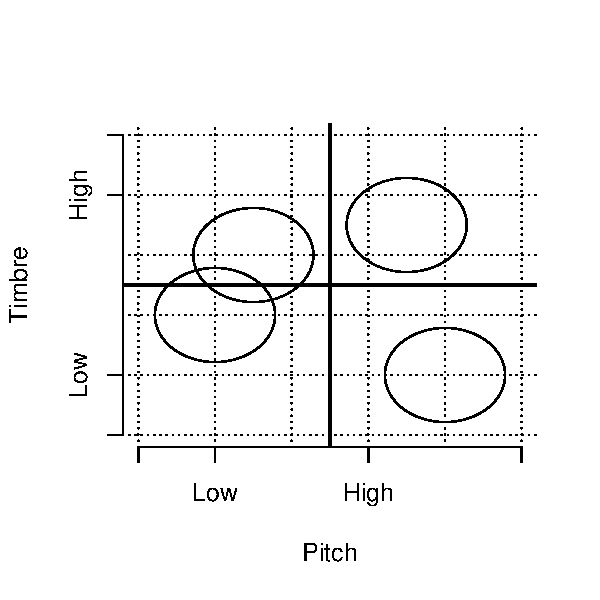
\includegraphics[width=\maxwidth]{figure/unnamed-chunk-11-1} 

\end{knitrout}
\caption{An example of a classic GRT model fitted to a 2X2 categorization data. Each of the stimuli are fitted with their own bivariate normal distribution.}
\label{fig:classicGRT}
\end{figure} 

Related difficulty is that it is hard to know, e.g. in the case depicted in Figure \ref{fig:classicGRT} which of the features of the data are purely coincidental and which of them accurately represent real dimensional interactions. Statistically speaking one could be \textit{overfitting}; a problem that is also recognized in the context of classic GRT models by \cite{soto2017}. Often the fit of the model is assessed by comparing the predicted response probabilities with the observed proportions (see for example \citet[Figure 4]{silbert2009}), but since separate distribution is used for each stimulus, the model is overly flexible, and it is unlikely that \textit{any} data set wouldn't be fit fairly well by it--using the criterion just discussed.

The current model rectifies these problems. Interactions are summarized by the $\kappa$ coefficients, so it's easy to make inferences. Since the model is constrained by the explicit functional relationship between signal levels and $d'$, it's less prone to the type of overfitting described. 

\paragraph{Process model}

The interactions in the model can be conceptualized by hypothesizing a process structure to the model, as in \cite{ashby1989}, \cite{ashby2000} or \cite{cohen2003}. This is demonstrated in Figure \ref{fig:GRTprocess}. On each channel the physical signal, $S$, is transduced to the internal representation of the signal, $s$, after which it is judged against the decisional criterion, $c$, and the participant gives their response, $R$. The straight lines from a stage to the next--for example from $S_x$ to $s_y$ denote an influence to the average level of the variable while curved lines inside a stage--for example from $s_y$ and $s_x$--denote correlated noise. 

The effect of the signal level on the average level of the internal signal on the other channel is usually referred to as stage 1 interaction, the correlation of noise between the internal representations is referred to as stage 2 interaction, and the the dependence of the criteria on the internal level of the signal or correlation between their noise is referred to as stage 3 interaction. Stage 1 and 2 interactions are referred to as \textit{perceptual} interactions, and stage 3 interaction is referred to as \textit{cognitive} interaction. \citep{ashby1989, ashby2000, cohen2003}. 

\begin{figure}[!htb]
\centering
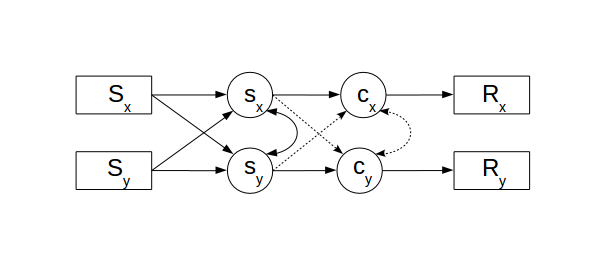
\includegraphics[scale = 0.8]{Process_model}
\caption{A process interpretation of the model. Variables inside rectangles are observed, whereas variables inside squares are latent. }
\label{fig:GRTprocess}
\end{figure}

In the current model, stage 1 interactions are modelled by the $\kappa$ terms while the stage 2 interaction is modelled by the correlation parameter $\rho$. Stage 3 interactions are not modelled, since, as the model currently stands, they are not identifiable. This issue will be discussed in greater detail later. 

\paragraph{Relationship to Generalized Linear Models}

Generalized Linear Models (GLM's) are widely implemented in statistical analysis (see e.g. \citet{kruschke2015, skrondahl2004}). The theoretical links to well-known models in statistics mean that the model should be easily generalizable to different situations, and that there exists a wide range of theoretical and empirical literature. 
 
\cite{decarlo1998} describes the unidimensional SDT model as a generalized linear model. In the case of normally distributed noise, a \textit{probit model}, which is how already Gustav Fechner--who is sometimes regarded as the founder of psychophysics--modelled categorical judgments in the 19th century (discussed in \citealt[Chapter 7]{stigler2003}). The relationship between the physical signal strength and the mean of the internal value being non-linear--see Equation \ref{eq:dprimefunc}--the model considered here is more accurately described instead as a \textit{non-linear} \citep[p. 379]{box2005} probit model. 

The model presented here can be thought of as a non-linear \textit{multinomial} probit model; in a binary choice probit model the responses are assumed to follow the binomial distribution, but in the multidimensional model, since there are more than two choices, the responses are assumed to follow the multinomial distribution \cite[p. ERROR]{skrondahl2004}. 

Due to this link to generalized linear models, the current approach is close to that used by \cite{cohen2003}. The most relevant difference is that \citeauthor{cohen2003} doesn't aim to model the functional relationships between the $d'$ values and the signal strengths, rather, he uses contrast coding, categorical stimuli and an identification task much like described earlier.

In the context of GLM's, the modelling of lapses is can be called \textit{robust regression} \citep[p. 635]{kruschke2015} since it relaxes the distributional assumptions somewhat, and isn't so prone to estimation errors due to outliers. However it should be noted that this requires the lapsing parameters to be fixed \citep[p. ERROR]{skrondahl2004}. This is not true for all of the models used in this thesis.

\subsubsection{Nonidentifiabilities and other limitations of the model}

\paragraph{What do the latent distributions really represent?}

The main assumption of SDT, and consequently GRT, is that the participant bases their decisions on noisy latent quantities. Therefore, it is important to discuss what those latent quantities actually represent.  

In SDT literature writers are generally careful to call the latent quantities evidence \citep{wickens2002, verde2006} or judgments (\citealp[p. 247]{stigler2003}). In GRT related literature, however, the latent quantities are thought to be more closely related perceptions. \cite{ashby2015} call them \textit{perceived values}; in \cite{ashby1986},  \cite{kadlec1992} and \cite{silbert2009} they are \textit{perceptual effects} and the space (in which the distributions are defined in) is defined as \textit{perceptual space}; \cite{soto2017} uses the term \textit{perceptual representation}.

As is clear from the preceding discussion on SDT and GRT, I've taken the more traditional way of calling the latent variables evidence, but even in this case one has to be careful in considering \textit{what} the evidence is about. Concretely the latent quantities are a sum of \textit{everything} that creates variability in responses: noise in encoding the signals, internal noise due to e.g. blood pressure or breathing, transient noises from sneezing or swallowing etc., lapses of attention, criterial changes, non-stationarity of threshold, effects of learning and so on. 

It is clear that for example in a pitch discrimination task many of the aforementioned factors don't necessarily directly effect the perceived amount of pitch difference, but can and will affect the judgments or amount of evidence in other ways, for example by masking the signal and limiting information that way.

Often there seems to be two strong implicit assumptions. First, that either the first factor alone or the two first would be significantly greater than any of the others, and second that any effect is sufficiently free from other influences. While these assumption might not be that dangerous in SDT models, the problem is exacerbated in GRT: there is virtually no information about how the aforementioned factors influence e.g. inferences about interactions between the dimensions, a problem recognized already by \citet{silbert2009}. It is my impression, based on my own unpublished simulation studies, that the factors just mentioned can in some situations lead to significantly incorrect inferences. 

Validity of the process model described earlier relies heavily on these strong assumptions and our ability to differentiate between different sources of variation. It is my belief that in the current formulation, using straightforward perceptual experiments, one can not properly identify these, and indeed has to rely on strong prior assumptions. For this reason I would, at this point, see the process model more as a helpful conceptualization than anything else.

Conceptualization of the latent variables affects the way interactions are understood theoretically. Based on the preceding discussion I hope it is clear that it is different to say that e.g. timbre influences the distribution of \textit{evidence} about pitch than it is to say that timbre influences the distribution of \textit{perceptual effects} of pitch.

\paragraph{Criterial noise}

Criterial noise can be defined as random variation in the criteria around some central value, in the present context the central value would most naturally be thought of as the parameter $c$ in the model. If this variation is assumed to be Gaussian, it is not identifiable from other sources. This issue has been discussed in SDT literature already by \cite{wickelgren1968}\footnote{\cite{wickelgren1968} talks about \textit{unidimensional strength theory}, but the discussion is directly applicable to the present situation.}; in the context of GRT \citet{ashby2000} has discussed the role of criterial noise. In the context of SDT there have been proposals for identifying the magnitude of criterial noise using experimental manipulations (see e.g. \citealt{kellen2012, benjamin2009, cabrera2015}), but the application of these methodologies to GRT will not be considered further here. 

In practice, any criterial noise will be included in the $\sigma$ estimates, since, as already discussed, these represent to sum total of all variation. With regard to GRT the problem is if the criterial noise between the dimensions is correlated: this will be included in the $\rho$ estimates. Another possibility is that criterial changes--e.g. between sessions or during a long session--would also affect the $\kappa$ estimates. To my knowledge, no systematic exploration of this possibility exists; in my own non-systematic simulations I have noticed that indeed in some cases such criterial shifts can affect the the parameter estimates and lead to false positives. 

\paragraph{Non-orthogonality of decisional boundaries}

Another topic tying into the modelling of decisional processing is the (possible) non-orthogonality of the decisional boundaries. In the GRT literature non-orthogonal decisional boundaries are seen as failure of \textit{decisional separability} \citep{ashby2015}, since the non-orthogonality implies that the decision is contingent on the level of the signal. 

In the present paper the focus is on orthogonal decisional boundaries. Non-orthogonal boundaries could be incorporated in the model, \cite{ennis2003} have shown a simple method for calculating the non-orthogonal integrals to evaluate the response probabilities. However, what could prove to be problematic is that the method, in my experience, is rather slow.  Another problem is the identifiability of non-orthogonal decisional boundaries: \cite{soto2015} claim that their model makes decisional separability identifiable--contrary to the classic model \citep{silbert2013}--but their result has been refuted on mathematical grounds by \cite{silbert2016}: any non-orthogonal boundaries can be thought of as a transformation of the space to one in which the boundaries are orthogonal and correlation between the dimensions changes. For this reason another way to look at the problem is to realize that any non-orthogonality will affect the $\rho$ parameter, and indeed if there is strong reason to believe such non-orthogonality exists, that should be taken into account when interpreting that particular parameter.  


\newpage

%Rnw root = "../Main.Rnw"

\section{Bayesian statistics}
\label{sec:bayes}

Bayesian statistics is at the core of this thesis: the adaptive algorithm to be used is based on the idea of representing uncertainty about parameters as probability distributions over them. Bayesian statistics will also be used for making inferences about data. In this section I will provide a short introduction to the central concepts that are needed for understanding the adaptive algorithm and, later, inferences made about the data. 

\subsection{Basics of Bayesian statistics}

The core idea of Bayesian statistics is the updating of prior information with observed data to arrive at a synthesis of them. This synthesis is called the posterior distribution. Both the prior information and the posterior distribution are represented as probability functions over the parameters, $\theta$. Equation \ref{eq:bayesprop} represents this process mathematically. \citep{kruschke2015}.

\begin{equation}
P(\theta | Data) \propto P(\theta) P(Data | \theta)
\label{eq:bayesprop}
\end{equation} 

$P(\theta | Data)$ is the posterior distribution, $P(\theta)$ is the prior distribution and $P(Data | \theta)$ is the likelihood function, i.e. the probability of observing the data given the parameter values.\footnote{In the full Bayes' theorem the posterior distribution is normalized with the integral over the possible observed values, $P(Data)$, assuring that it always integrates to one and is a proper probability distribution: $P(\theta | Data) = (P(\theta) P(Data | \theta)) / P(Data)$ \citep{kruschke2015}, but I think the equation without the normalizing constant captures the main idea more clearly. This is why the symbol $\propto$ ("proportional to") is used in Equation \ref{eq:bayesprop}.}

Updating is demonstrated for a single parameter in Figure \ref{fig:priorpost}. The shaded region represents the prior distribution $P(\theta)$, which in this case, is a log-normal distribution.  After some data has been observed the prior distribution is updated with evidence, $P(Data | \theta)$, represented by the dashed line, which then results in the posterior distribution $P(\theta | Data)$, represented by the solid line. Observing data, in this particular case, has reduced our uncertainty about likely values for the parameter $\sigma$, the probability density has become more concentrated.

\begin{figure}
\centering
\begin{knitrout}
\definecolor{shadecolor}{rgb}{0.969, 0.969, 0.969}\color{fgcolor}
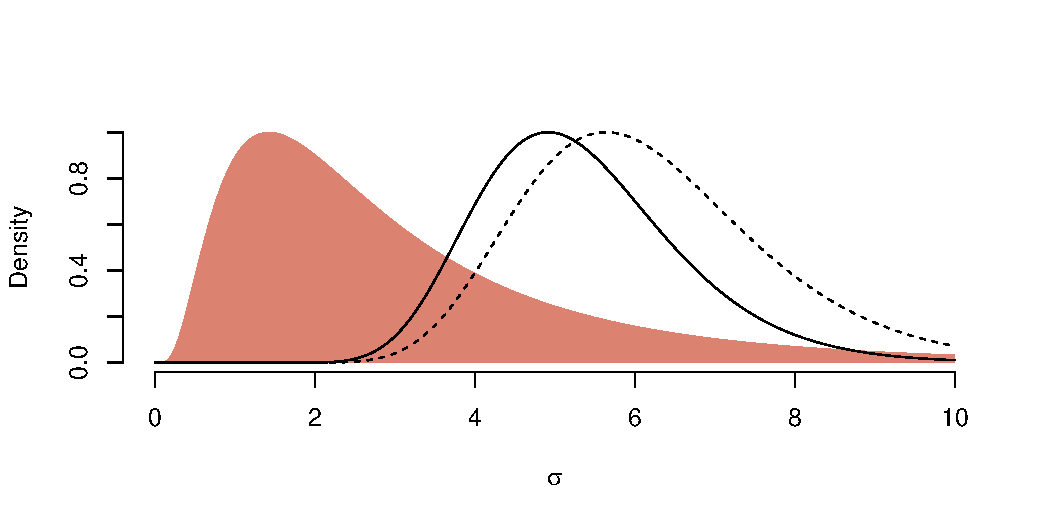
\includegraphics[width=\maxwidth]{figure/unnamed-chunk-12-1} 

\end{knitrout}
\caption{A simplified example of the basic concepts of Bayesian inference. The shaded area represents prior knowledge about the parameter $\sigma$. Dashed line is $P(Data | \theta)$ and the solid line is the posterior probability density, $P(\theta | Data)$}
\label{fig:priorpost}
\end{figure}

Of course, in models of any complexity prior and posterior probability densities are defined over a multidimensional space. In this thesis the dimensionalities range from 7 to 27. 

The term $P(Data | \theta)$ defines how the model learns from data, and is usually called \textit{likelihood} \citep{kruschke2015}. Also, for numerical stability, likelihood is usually defined using logarithms of probabilities. Here, the likelihood for a particular $\theta$ is simply the sum of the logarithms of the probabilities of the observed  responses and signals: (for a similar approach see \citet[p. 218]{wickens1992}):

\begin{equation}
\sum_{t=1}^n ln P(\bm{R}^t, \bm{S}^t; \theta)
\end{equation}

This is the generic expression for  all models in this essay. The probabilities are always calculated by using the specific formulae defined earlier for a given model. 

\subsection{Hierarchical models}
\label{sec:hierarchical_models}

The term \textit{hierarchical model} can refer to many different kinds of models\footnote{Andrew Gelman has collected a bunch of different names for hierarchical models in to a blog post: https://statmodeling.stat.columbia.edu/2019/09/18/all-the-names-for-hierarchical-and-multilevel-modeling/}. I will be using two kinds of hierarchical models: 1) Model in which the parameters are assigned distributions 2) Models embedded in a higher level mixture model. Both kinds of models will be discussed separately.

\subsubsection*{Models in which parameters have distributions}

Often these kinds of models are described as being models in which priors have (hyper)priors (e.g. \citet[p. 225]{kruschke2015} talks about \textit{". . . hierarchical chain of dependencies among parameters."}). However, I think it's clearer to think this as an extension of fitting e.g. multiple linear models to different data sets. Instead it is possible to group models together on a higher level, and assign the groups of parameters (e.g. all intercepts from all of the models) probability distributions. This is sometimes known has \textit{random effects modelling} in the frequentist setting.

The general idea is demonstrated in Figure \ref{fig:hierarchical_model_for_groups}. The index $i$ is an index for the \textit{group} to which the observation $y_{ij}$ belongs to, $j$ indexing observations inside that group. Each group then gets a unique set of parameters of the linear function. These parameters are each assigned a distribution (prior), which in this case is the normal distribution, whose parameters are unknown and are inferred from the data. Note that for the $\sigma$ parameters the normal distributions are truncated at zero. At the highest level each parameter of these distributions gets a hyperprior, which in this case for each parameter is the standard normal distribution--taking into account again that $\sigma$ is truncated at zero.

\begin{figure}[!htb]
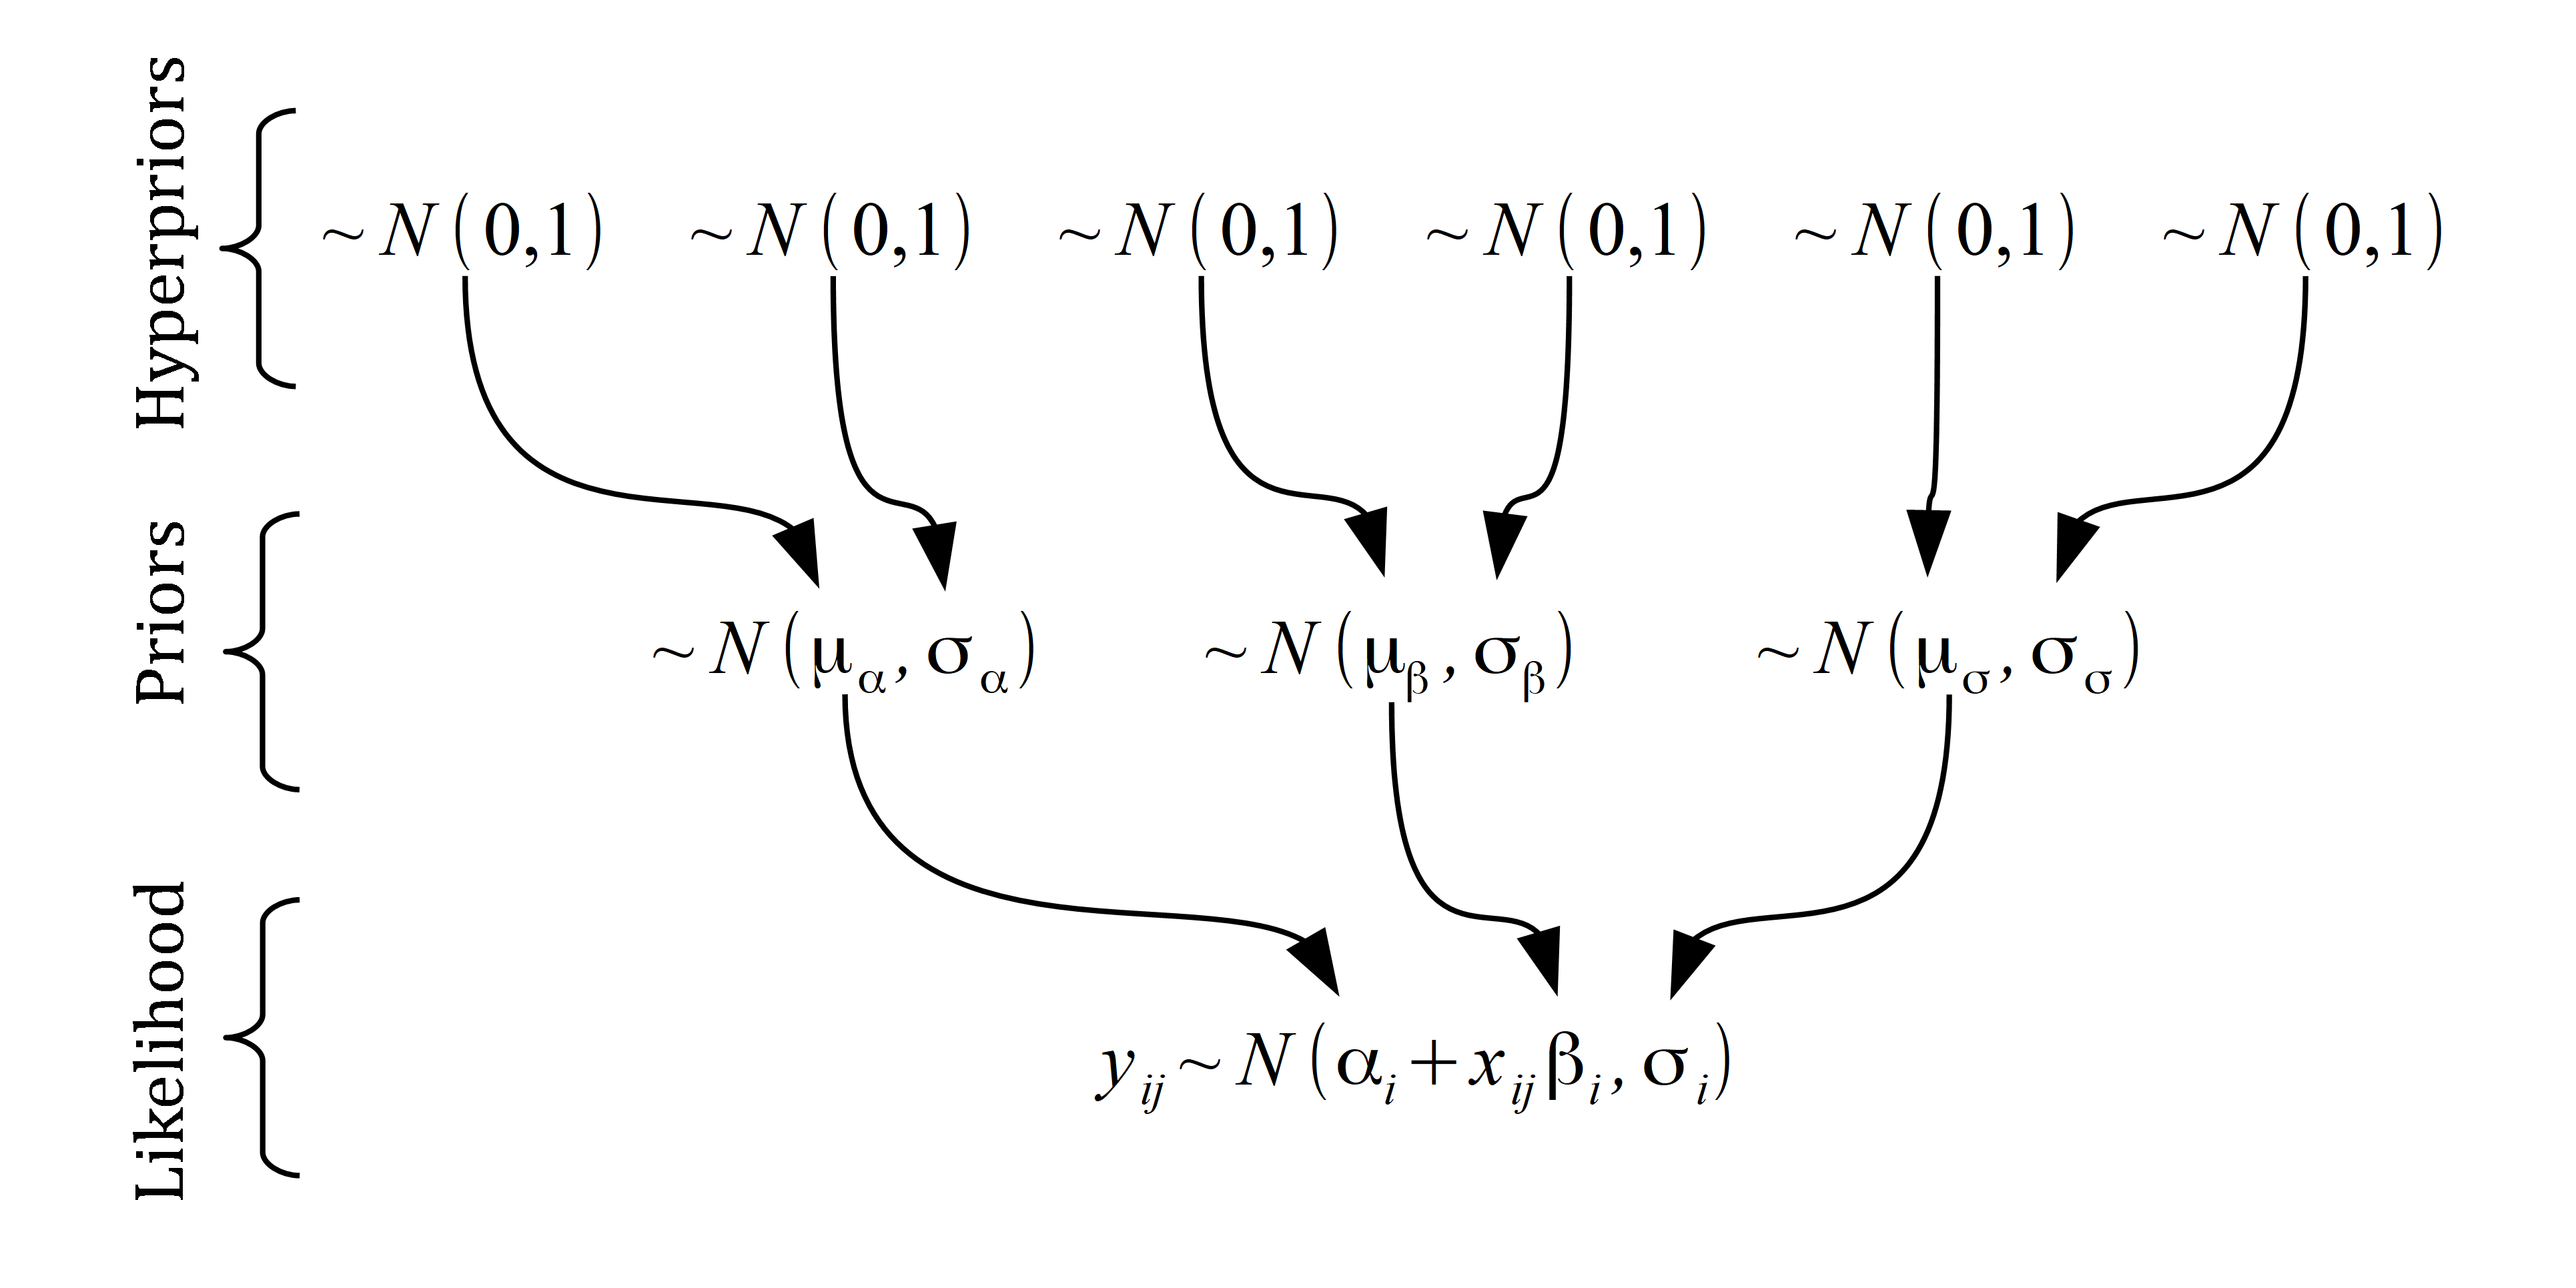
\includegraphics{Hierarchical_model_for_groups}
\caption{A schematic illustration of a hierarchical linear model in which each of the parameters is given a distribution for which the parameters are inferred from the data. This creates a distinct multilevel structure to the model.}
\label{fig:hierarchical_model_for_groups}
\end{figure}

Since the parameters are related on a higher level, some information is shared between them. One feature is that all of the means are adjusted towards the common mean, which functions analogously to multiple comparisons adjustments in frequentist statistics \citep{gelman2012}. 

\subsubsection*{Models embedded in a mixture model} 

Often the same data set can be fit by multiple models. These are sometimes also called \textit{mixture} models, since the idea is to model psychophysical data as a mixture of different models. I will begin by describing a simple two-level model. This corresponds with how lapsing behaviour is often modelled in the psychophysical literature. I will then introduce a three-level model which is used here to combine the models with different types of interference ($\kappa_{\mu}$/$\kappa_{\sigma}$) in one model.  

\paragraph{Two-level model}

A simple two-level model is presented in figure \ref{fig:Basic_hierarchical_model}. At the lowest level, the figure shows two models, one labelled \textit{lapses} and the other \textit{cognitive}, embedded in a higher level model. Both of the lower level models aim to explain the same set of observations, $y_1, y_2 \dots y_i$, the $y$ terms, in this case, consisting of pairs of stimuli ($\bm{S} = [S_x, S_y]$) and responses ($\bm{R} = [R_x, R_y]$). 

\begin{figure}[!htb]
\begin{center}
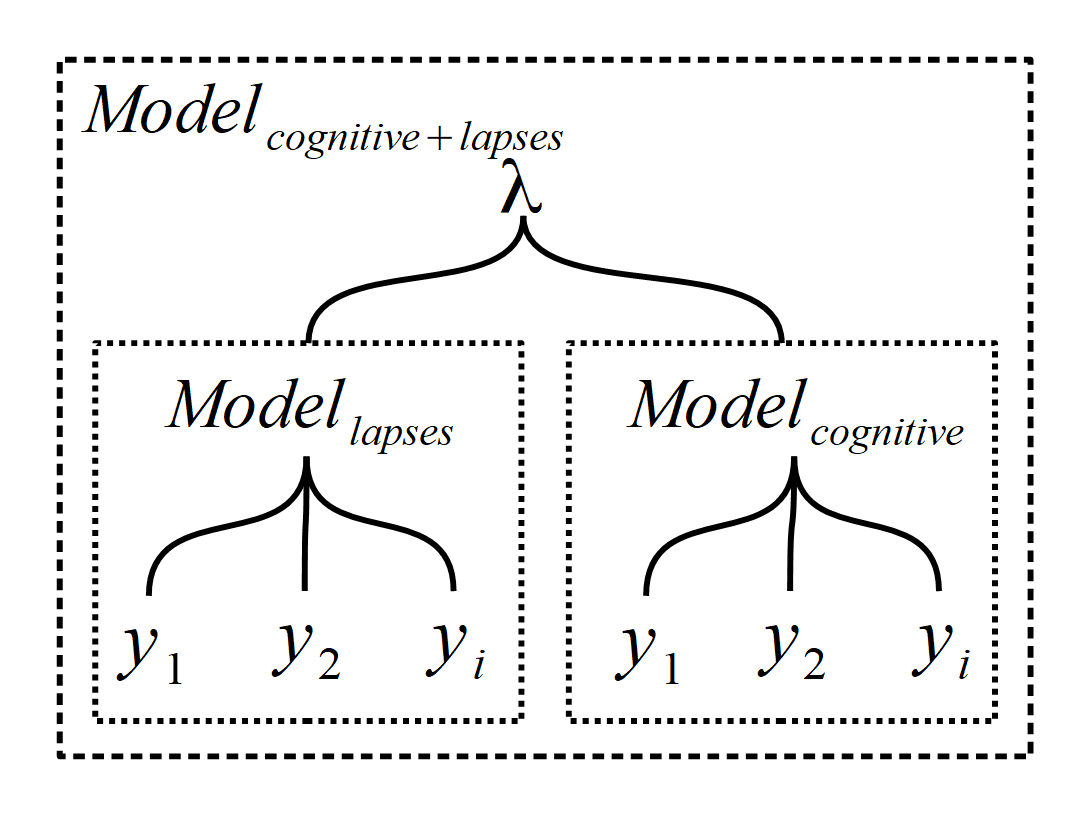
\includegraphics[scale=0.75]{Basic_hierarchical_mixture_model}
\end{center}
\caption{A simple hierarchical model, which shows how the two models, one modelling lapses and the other the cognitive processes of interest, are related on a higher level through the coefficient $\lambda$.}
\label{fig:Basic_hierarchical_model}
\end{figure}

The cognitive model can be any of the models defined in section ERROR. The lapsing model, which was described in more detail in section ERROR, is defined by the single parameter $\gamma$, which is a multinomial distribution containing the response probabilities for the individual response categories. These probabilities do not depend on the signal levels, or in fact, on anything else outside them (see Section \ref{sec:modelling_responses} \textit{\nameref{sec:modelling_responses}} for how the responses are coded):

\begin{equation}
P(y_i)=
\begin{cases}
  \gamma_1, & \text{if } \bm{R} = [-1, -1]\\
  \gamma_2, & \text{if } \bm{R} = [\phantom{-}1, -1]\\
  \gamma_3, & \text{if } \bm{R} = [-1, \phantom{-}1]\\
  \gamma_4, & \text{if } \bm{R} = [\phantom{-}1, \phantom{-}1]
\end{cases}
\end{equation}

This simply says that if, for example, on a certain trial the response $[1,-1]$ is observed, the likelihood is incremented by $\gamma_2$. I will be assuming that all responses are as likely, i.e. $\gamma = [0.25, 0.25, 0.25, 0.25]$. This implies that the parameters of the lapsing model are not inferred from the data, partially due to the aforementioned (see Section \ref{sec:lapses_general} \textit{\nameref{sec:lapses_general}}) difficulty of inferring details of lapsing behaviour from psychophysical data. This is a very common way of including model of lapses, see e.g. ERROR ERROR ERROR.

The contributions of these two models are defined by the coefficient $\lambda$, which defines the weight of each model to the total likelihood:

\begin{multline}
\label{eq:lower_level_hiera}
P(y_i |\Theta_{\text{cognitive + lapses}}, \text{Model}_{\text{cognitive + lapses}}) = \lambda P(y_i | \theta_{\text{lapsing}}, \text{Model}_{\text{lapsing}}) + \\ (1 - \lambda) P(y_i | \theta_{\text{cognitive}}, \text{Model}_{\text{cognitive}})
\end{multline}

The vector $\Theta_{\text{cognitive + lapses}}$ contains all of the parameters for the lower level models and $\lambda$: $\Theta_{\text{cognitive + lapses}} = [\lambda, \theta_{\text{lapsing}}, \theta_{\text{cognitive}}]$.

\paragraph{Three-level model}

The three level model used here combines a pair of the two-level models at a higher level. Figure \ref{fig:Structure_of_hierarchical_model} show this schematically. The lower level models (in the two horizontally aligned boxes at the bottom) correspond to the structure shown in Figure \ref{fig:Basic_hierarchical_model}. However, here the individual models are labelled according to the specific cognitive model they are using. 

\begin{figure}[!htb]
\begin{center}
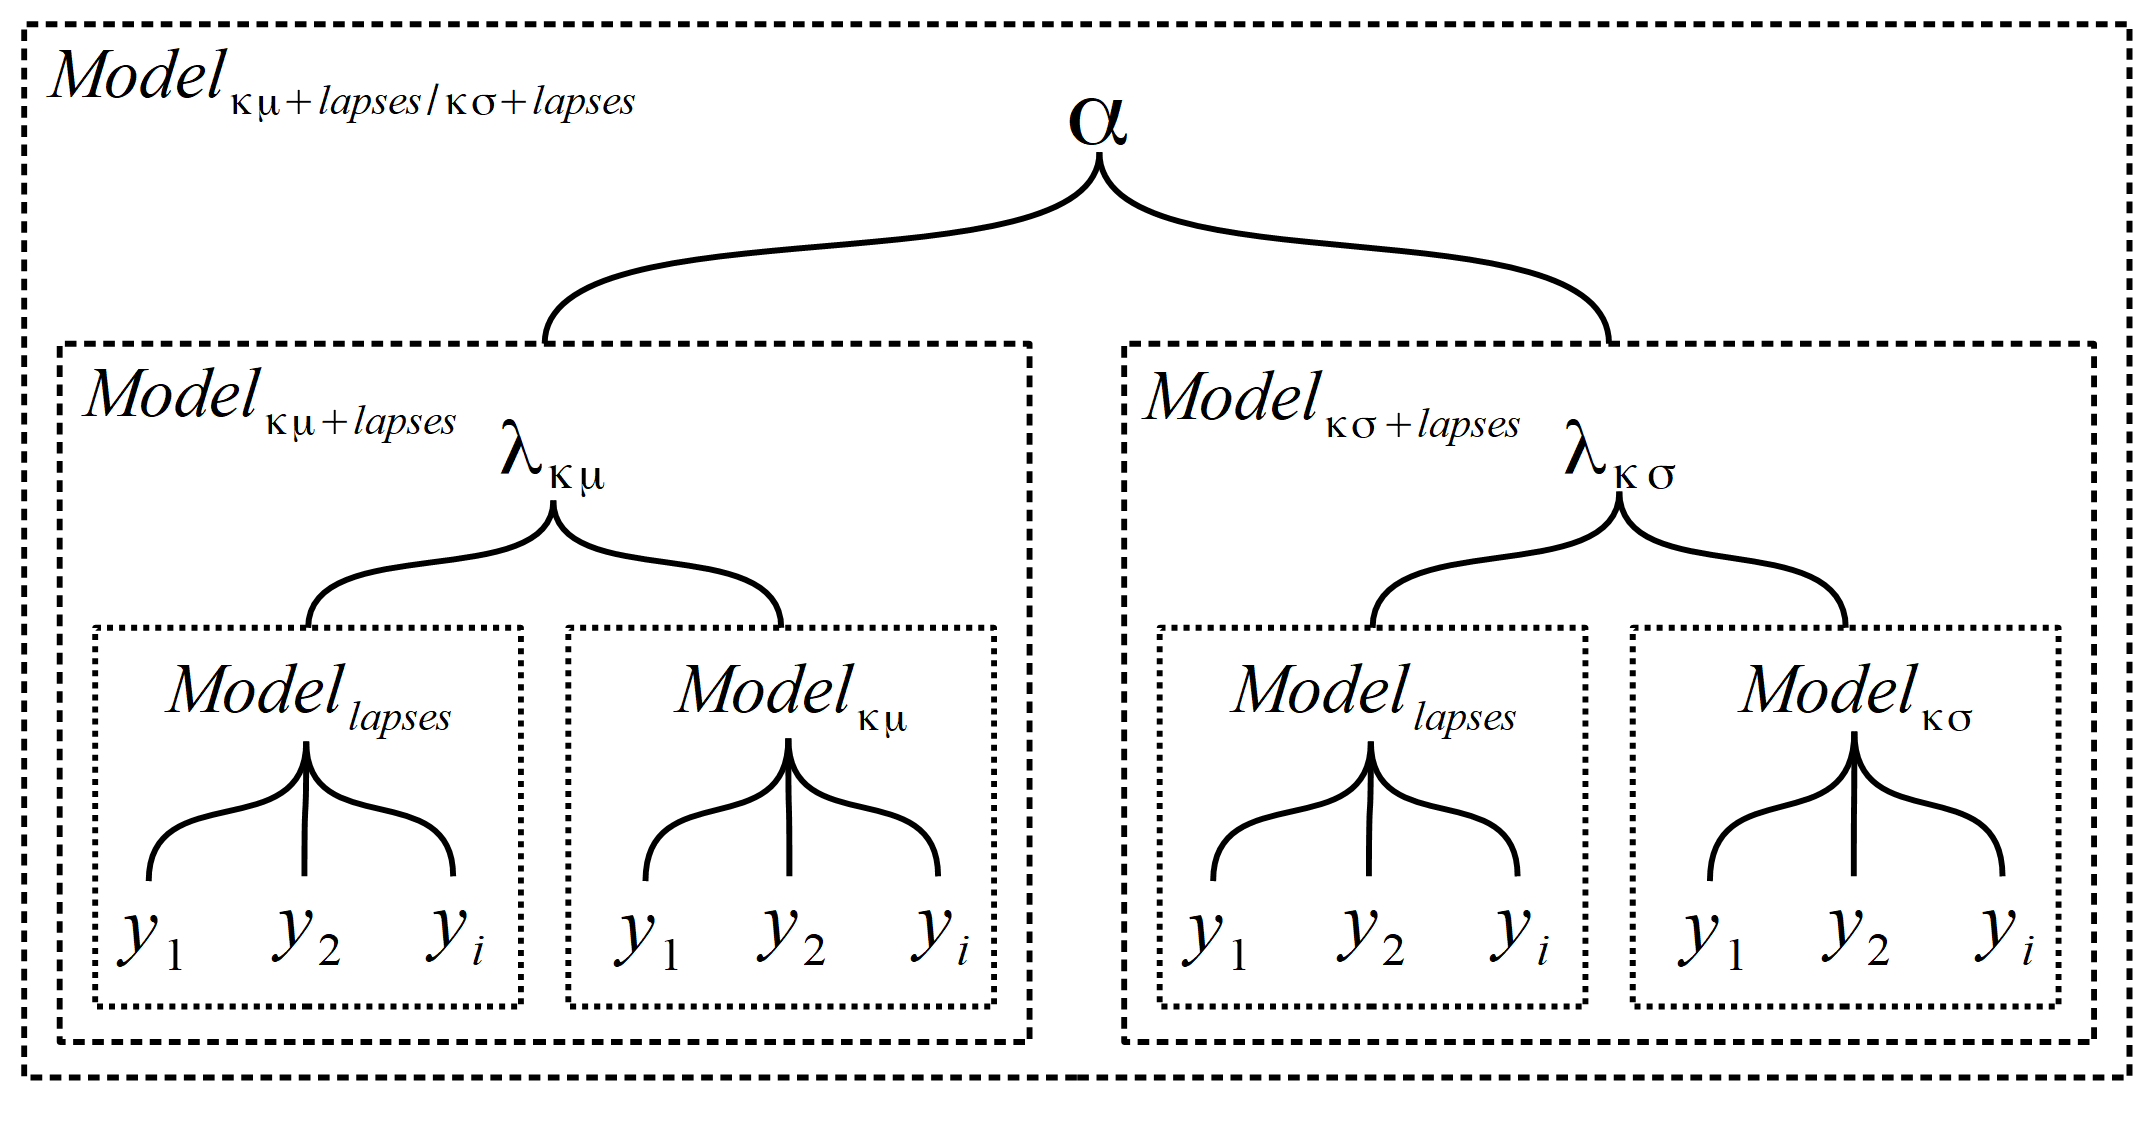
\includegraphics[width=\textwidth]{Structure_of_hierarchical_mixture_model}
\end{center}
\caption{Structure of the hierarchical model used in this work. On the highest level the $\alpha$ coefficient combines the models with different models for interactions.}
\label{fig:Structure_of_hierarchical_model}
\end{figure}

Similar to the parameter $\lambda$ in the two-level case, here the contributions of the two lower level hierarchical models are modelled by the parameter $\alpha$. The likelihood is

\begin{multline}
P(y_i |\Theta_{\kappa \mu + \text{lapses} / \kappa \sigma  + \text{lapses}}, \text{Model}_{\kappa \mu + \text{lapses} / \kappa \sigma  + \text{lapses}}) = \alpha P(y_i |\theta_{\kappa \mu + \text{lapses}} \text{Model}_{\kappa \mu + \text{lapses}}) + \\ (1 - \alpha) P(y_i |\theta_{\kappa \sigma  + \text{lapses}}, \text{Model}_{\kappa \sigma  + \text{lapses}})
\end{multline}

in which the likelihoods for the lower level models are defined in equation \ref{eq:lower_level_hiera}.

\subsection{Bayesian inference in the General Recognition Theory}

In this work Bayesian approach is also used during the analysis of the data. Classic GRT studies have been dominated by frequentist methods, and e.g. definitions of interactions have relied on testing for the statistical significance of the parameter values associated with them (e.g. \cite{ashby2015, wickens1992}), to my knowledge, \cite{silbert2010} is the only GRT related work using Bayesian analysis framework. Contrary to the majority of studies, I won't be doing any explicit significance tests, nor am I using the usual \textit{Type I/II} error framework \citep[pp. 470 - 471]{christensen1997}, since there are many problems associated with this.

For example if interactions are selected based on their statistical significance, effect sizes are likely to be exaggerated \citep{gelman2018}; but the more damning criticism is that the $p$-value doesn't differentiate between \textit{effect} or \textit{no effect} (\cite{greenland2016}), i.e. between \textit{interaction} or \textit{no interaction}, and in general, there has been a substantial amounts of criticism targeted towards focusing on binary decisions based on \textit{p}-values and instead a push to instead focus on the effect sizes and uncertainties associated with them (see e.g. \citet{kline2004, greenland2016, steiger1997}). 

This shift should not be seen only as a trivial data analytical decision: it should be seen as reflecting a wider push in the behavioural sciences to move away from binary decisions (see e.g. \citet{amrhein2017}), and--in the light of the topic--relating to the interpretation of interactions as being graded properties of the stimuli (as discussed in \citet{kemler1993}), instead of something that either is or isn't.

\newpage

%!Rnw root = ../Main.Rnw

\section{Simulations}
\label{sec:simulations}

I will be considering two main questions: 

\begin{enumerate}
  \item How much more efficient the adaptive algorithm is in relation to sampling stimuli from a fixed grid--if at all? 
  \item How well can generating parameters be recovered?
\end{enumerate}

These questions are closely related, since relative efficiency of the algorithms (Question 1) is defined here by the quantities that are also used to evaluate Question 2. 

There are two quantities of interest. First is defined by taking the means of the marginal posterior distributions as point estimates and calculating the squared differences to the generating parameters. This quantifies squared bias and variance of these estimators. The second quantity is the standard deviations of the marginal posterior distributions. This is used as a measure of how much uncertainty about the parameters is left after the data collection process. The goal, as already stated, is to minimize uncertainty about the parameters.

Question 1 is evaluated by inspecting if there are differences between the algorithms in how quickly the aforementioned quantities approach zero. Question 2 is answered by looking at the same  quantities, but the focus is on the overall performance, not differences. The first question is more closely related to the topic of this thesis, but the second question has more general value regarding the estimation of GRT models for which reason it can't be ignored. 

\subsection{Methods}

The general method was the following: first a set of generating parameters for the simulated observer were drawn randomly, and then either of the algorithms (adaptive/non-adaptive) described earlier were run. This was done for both the Yes/No and 21-4AFC procedure, resulting in four different conditions\footnote{There was a third algorithm, that consisted of sampling stimuli randomly from an adaptive grid, but results from this condition are not reported here, since it doesn't directly answer the main question posed in this thesis. The interested reader can find the data and R code to plot the results from: \url{https://github.com/joanpaak/Master_thesis}}. 

I have chosen the number 800 fairly arbitrarily; it represents a number of trials that, I think, could still be administered relatively continuously to a participant, without taking into account non-stationarities induced by a multi-session design. I have tried to pick a number that would b large enough; if one thinks that the number is lower, one can still get that information from the graphs. 

\paragraph{Prior distributions}

Prior distributions and distributions from which generating parameters for the simulations were drawn from are shown in Figure \ref{fig:priors} and in tabular form in Table \ref{tab:priors}. The same prior and generating distribution is used for both dimensions. Note that the scale for criterion is given in false alarm probabilities for easier interpretation. 

Priors for the parameters were chosen based on prior information from \citet{silbert2009} and from pilot testing. 

Prior for $\sigma$ was chosen to be fairly vague to reflect the possibility of widely differing thresholds.

Generating parameters for the simulations were drawn from bimodal distributions. The idea was to draw values that are covered by the prior, but which do not necessarily correspond with the mode of the prior distribution. Another motivation was to have qualitatively different simulated observers: some that have high values for some of the parameters and others that have low values.

\begin{figure}[!htb]
\centering
\begin{knitrout}
\definecolor{shadecolor}{rgb}{0.969, 0.969, 0.969}\color{fgcolor}
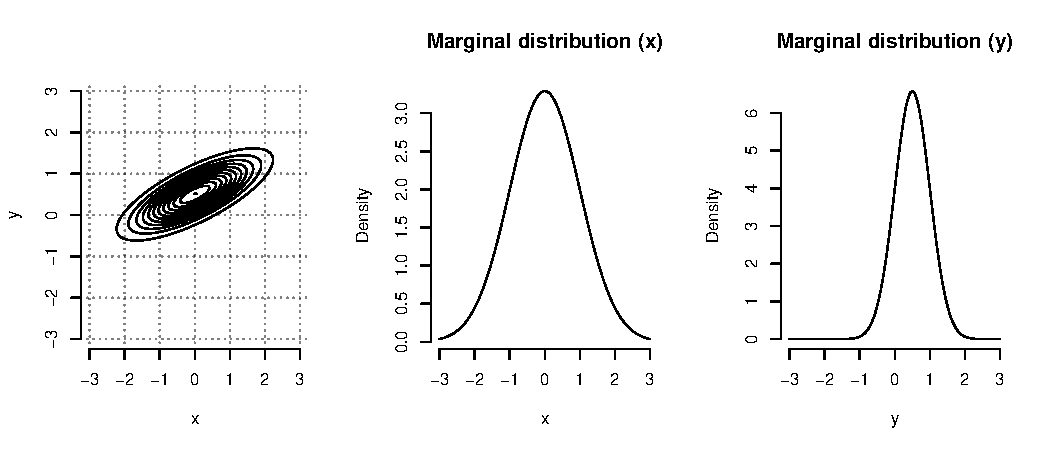
\includegraphics[width=\maxwidth]{figure/unnamed-chunk-13-1} 

\end{knitrout}

\caption{Prior distributions for the parameters of the model (solid black lines) and distributions for generating parameters for the simulations (regions shaded with red). Note that all of the densities are normalized to have maximum value of 1.0.}
\label{fig:priors}
\end{figure}

\begin{table}[H]
\centering
\caption{Parameters used for prior distributions and distributions of generating parameters. $M^l$ and $M^u$, respectively, are for the lower and upper peaks of bimodal distributions.}
\vspace{0.5cm}
\begin{tabular}{cccccc}
\toprule

          & \multicolumn{2}{c}{Prior} & \multicolumn{3}{c}{Generating}   \\
          \cmidrule(lr){2-3}\cmidrule(lr){4-6}
          & $M$       & $SD$    & $M^l$         & $M^u$         & $SD$   \\
\midrule
$\sigma$  & $log(2.5)$  & $0.75$   & $log(1)$    & $log(5)$    & $0.08$ \\
$C$       & $1.5$            & $0.3$   & $1.2$         & $1.7$         & $0.05$  \\
$\beta$   & $log(1)$  & $0.3$   & $log(0.8)$    & $log(1.2)$    & $0.05$ \\
$\kappa$  & $0$            & $0.3$   & $-0.25$        & $0.25$         & $0.075$ \\
$\rho$    & $0$            & $0.7$  & $atanh(0.75)$ & $atanh(-0.25)$  & $0.1$ \\
\bottomrule
\end{tabular}
\label{tab:priors}
\end{table}

\subsection{Results}

Total number of simulations per condition are shown in Table \ref{tab:conditions}. Squared errors and marginal standard deviations are presented in two ways: 1) on trial-by-trial basis and 2) by estimating the average differences on the last trial.

\begin{table}[H]
\centering
\caption{Conditions and number of simulations in each.}
\vspace{0.5cm}
\begin{tabular}{ccc}

\toprule
Procedure & Algorithm & N \\
\midrule
Yes/No & Adaptive & 184 \\
Yes/No & Random & 284 \\
2I-4AFC & Adaptive & 174 \\
2I-4AFC & Random & 130 \\

\bottomrule

\end{tabular}

\label{tab:conditions}
\end{table}

\paragraph{Trial-by-trial estimates}
Trial-by-trial results from the simulations are summarized in Figures \ref{fig:simulation_YN_sensory_sq_error} to \ref{fig:simulation_AFC_interaction_SD}. The figures show squared errors in relation to generating parameters and marginal standard deviations after $N$ trials, all the way to trial number 800. In all plots black color is used for the randomly sampled stimuli while red is used for adaptively sampled stimuli. The shaded regions indicate 50\%-quantiles (from 25\% to 75\%); solid lines indicate medians. Sensory ($\sigma$, $\beta$, crit) and interaction ($\kappa_{\mu}$, $\rho$) are shown in their own figures.

\begin{figure}[H]
\centering
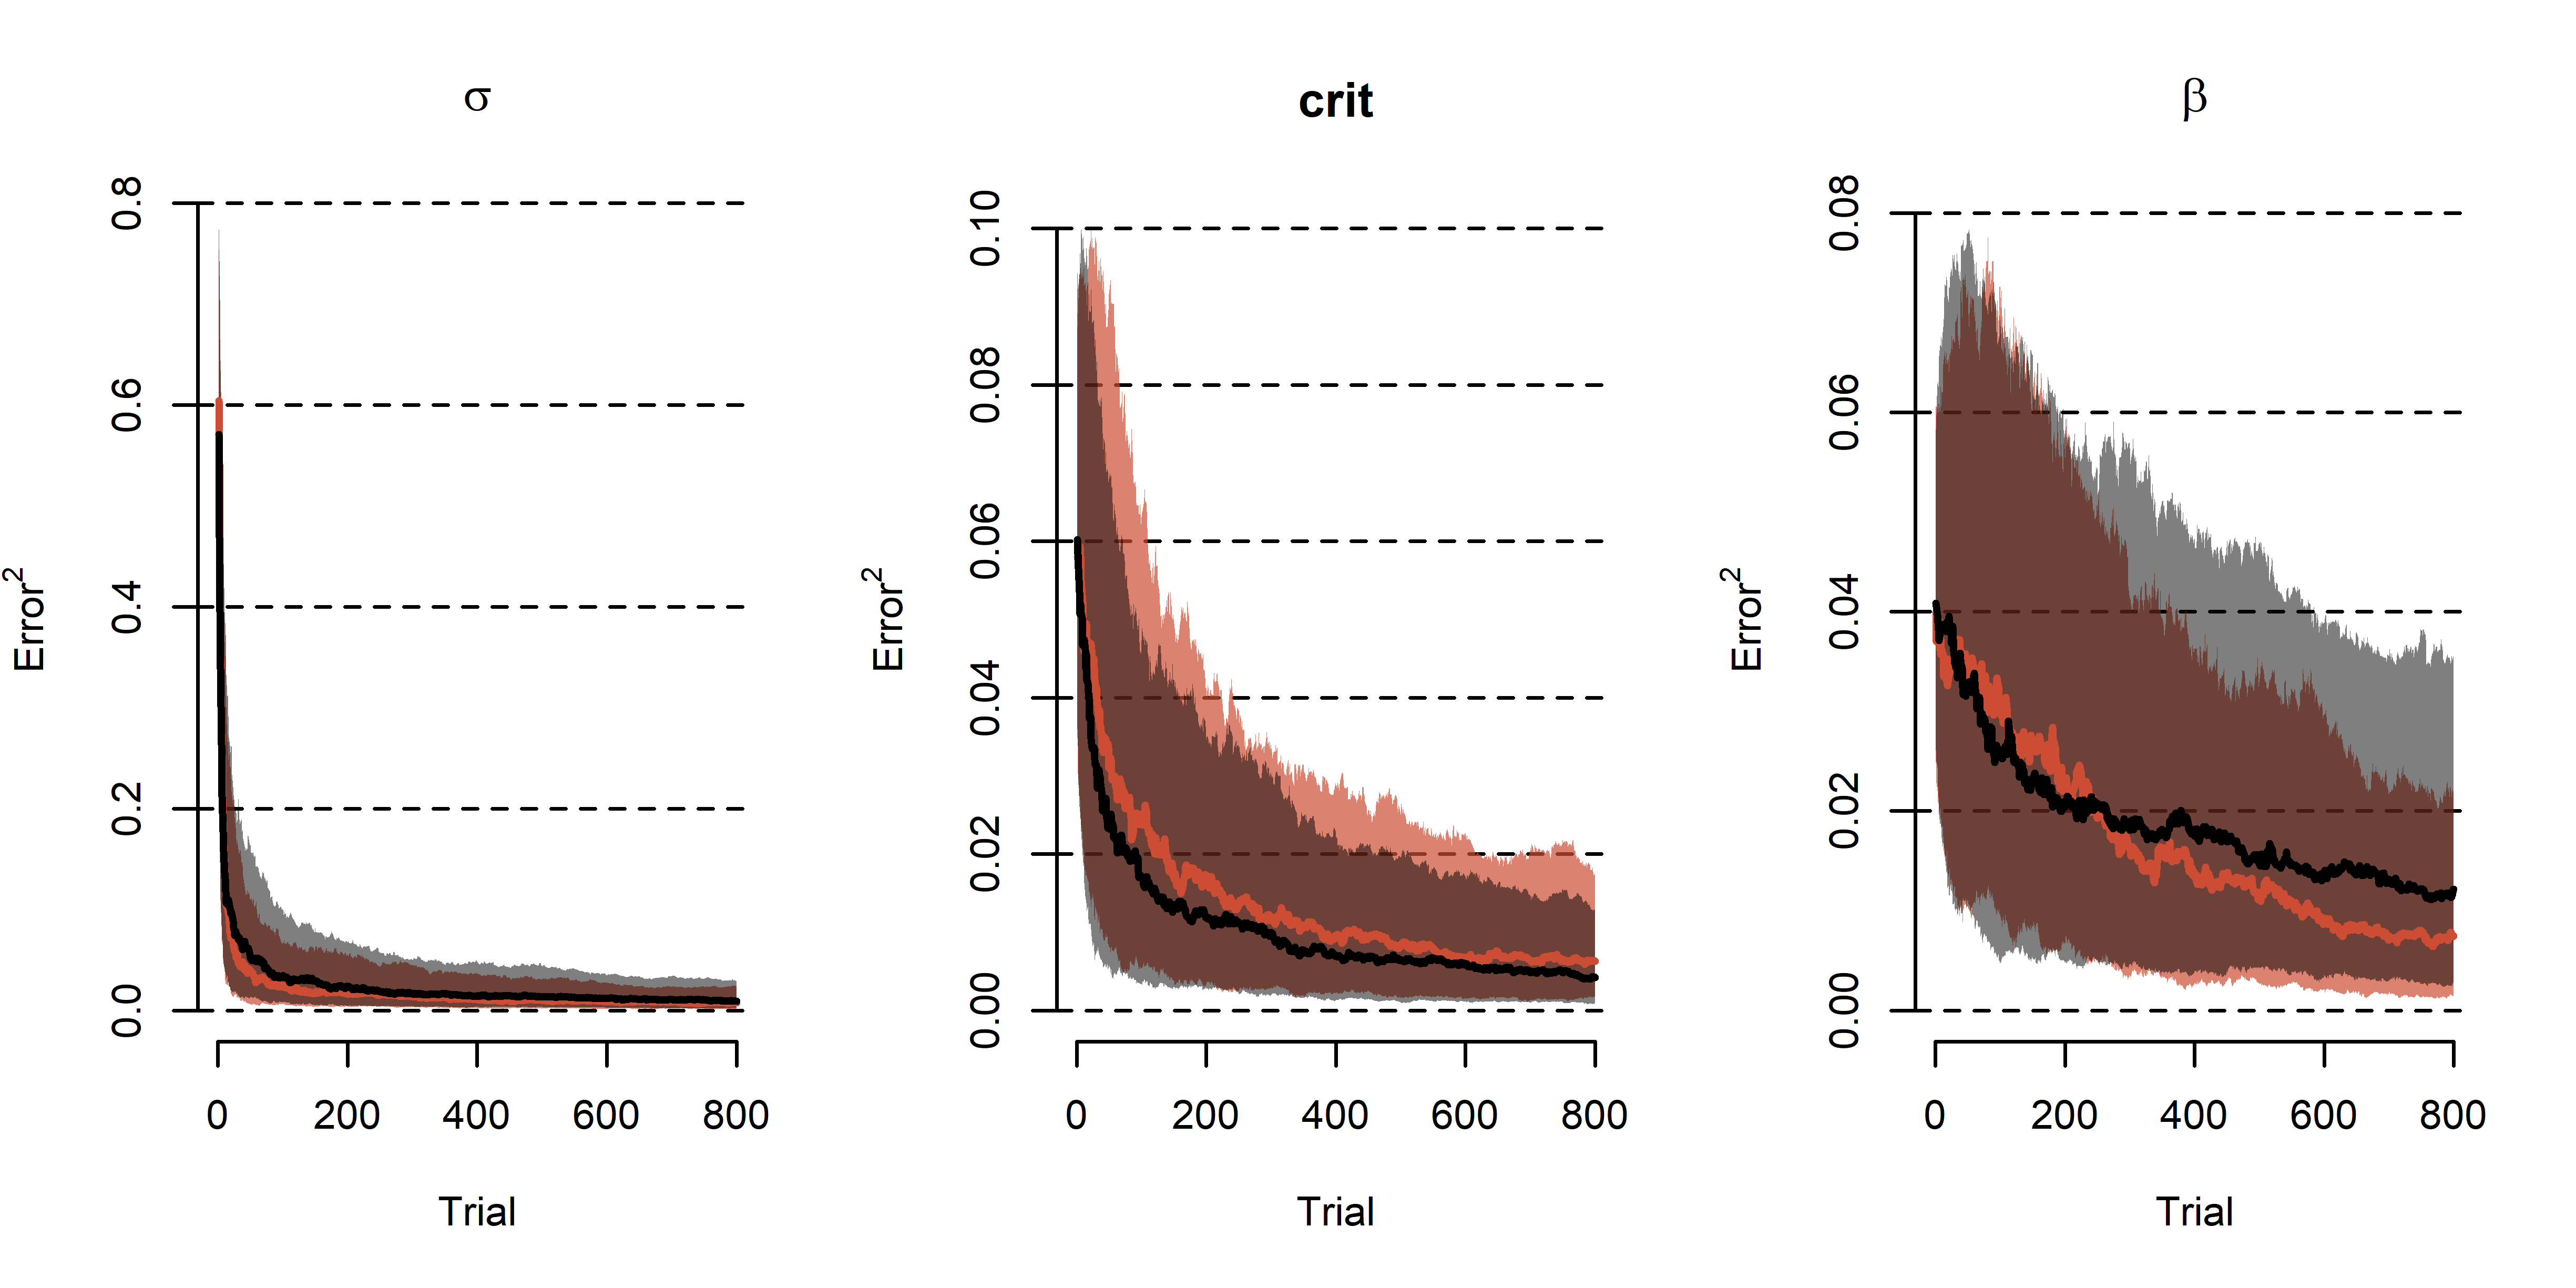
\includegraphics[scale=0.75, angle = 0]{simulation_YN_sensory_sq_error}
\caption{Procedure: Yes/No; sensory parameters. Trial-by-trial squared error between marginal means of the posterior distribution and generating parameters. Red: adaptive algorithm; black: random stimuli.}
\label{fig:simulation_YN_sensory_sq_error}
\end{figure}

\begin{figure}[H]
\centering
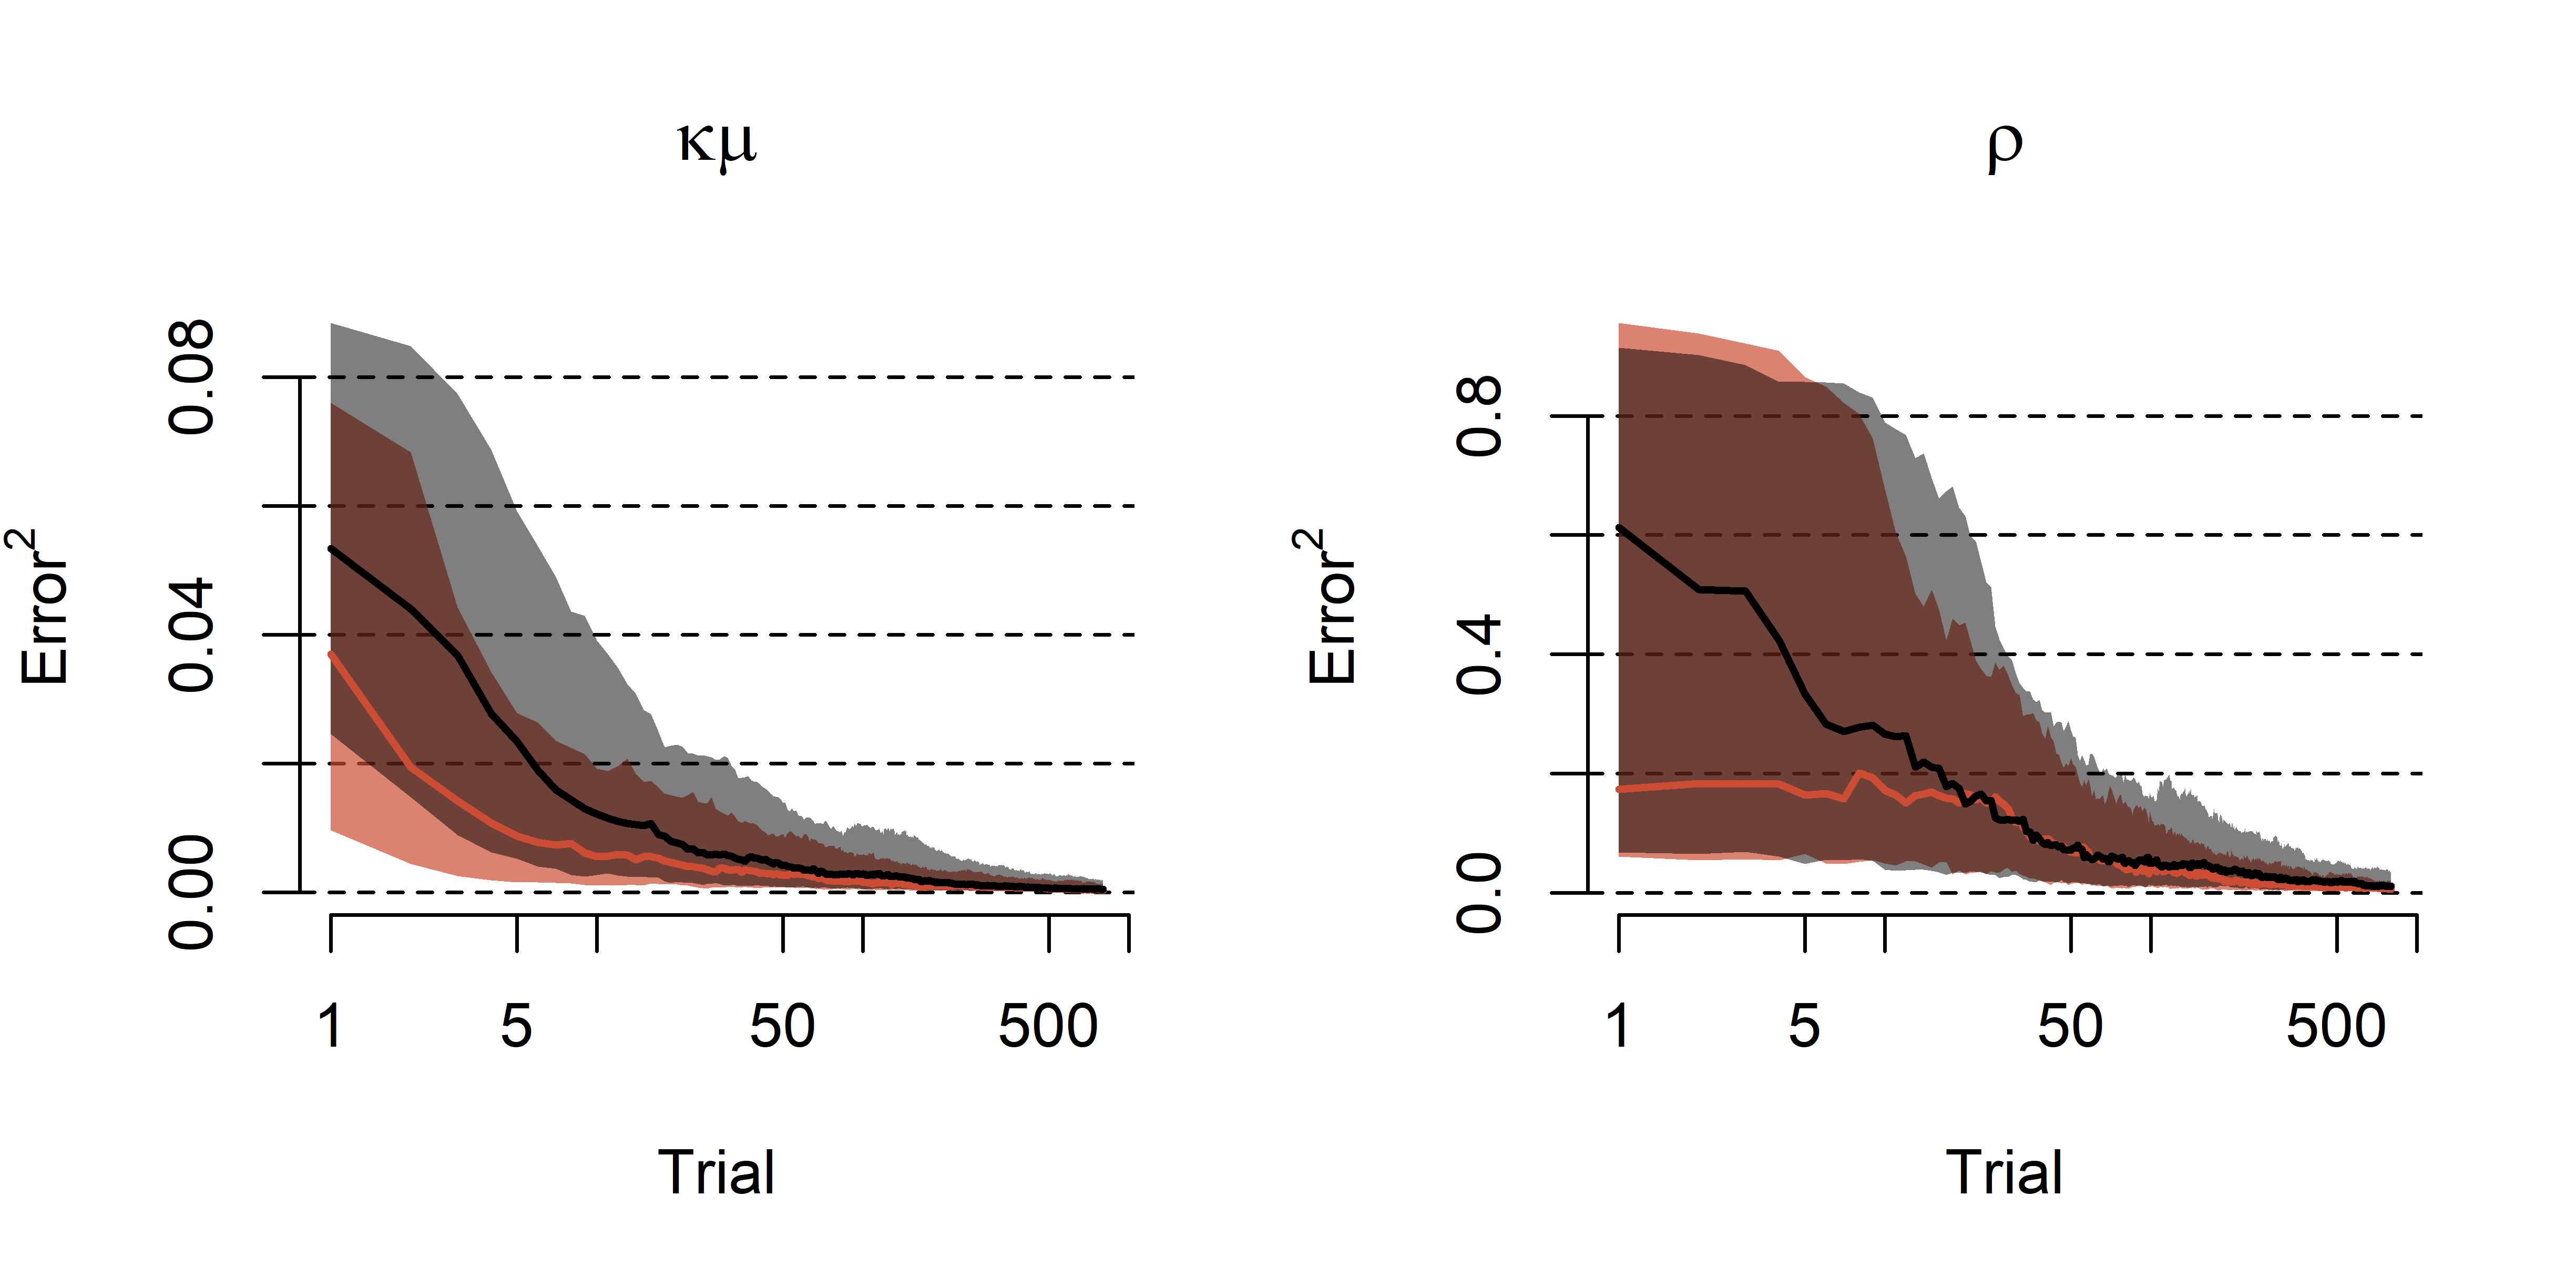
\includegraphics[scale=0.75, angle = 0]{simulation_YN_interaction_sq_error}
\caption{Procedure: Yes/No; interaction parameters. Trial-by-trial squared error between marginal means of the posterior distribution and generating parameters. Red: adaptive algorithm; black: random stimuli.}
\label{fig:simulation_YN_interaction_sq_error}
\end{figure}

\begin{figure}[H]
\centering
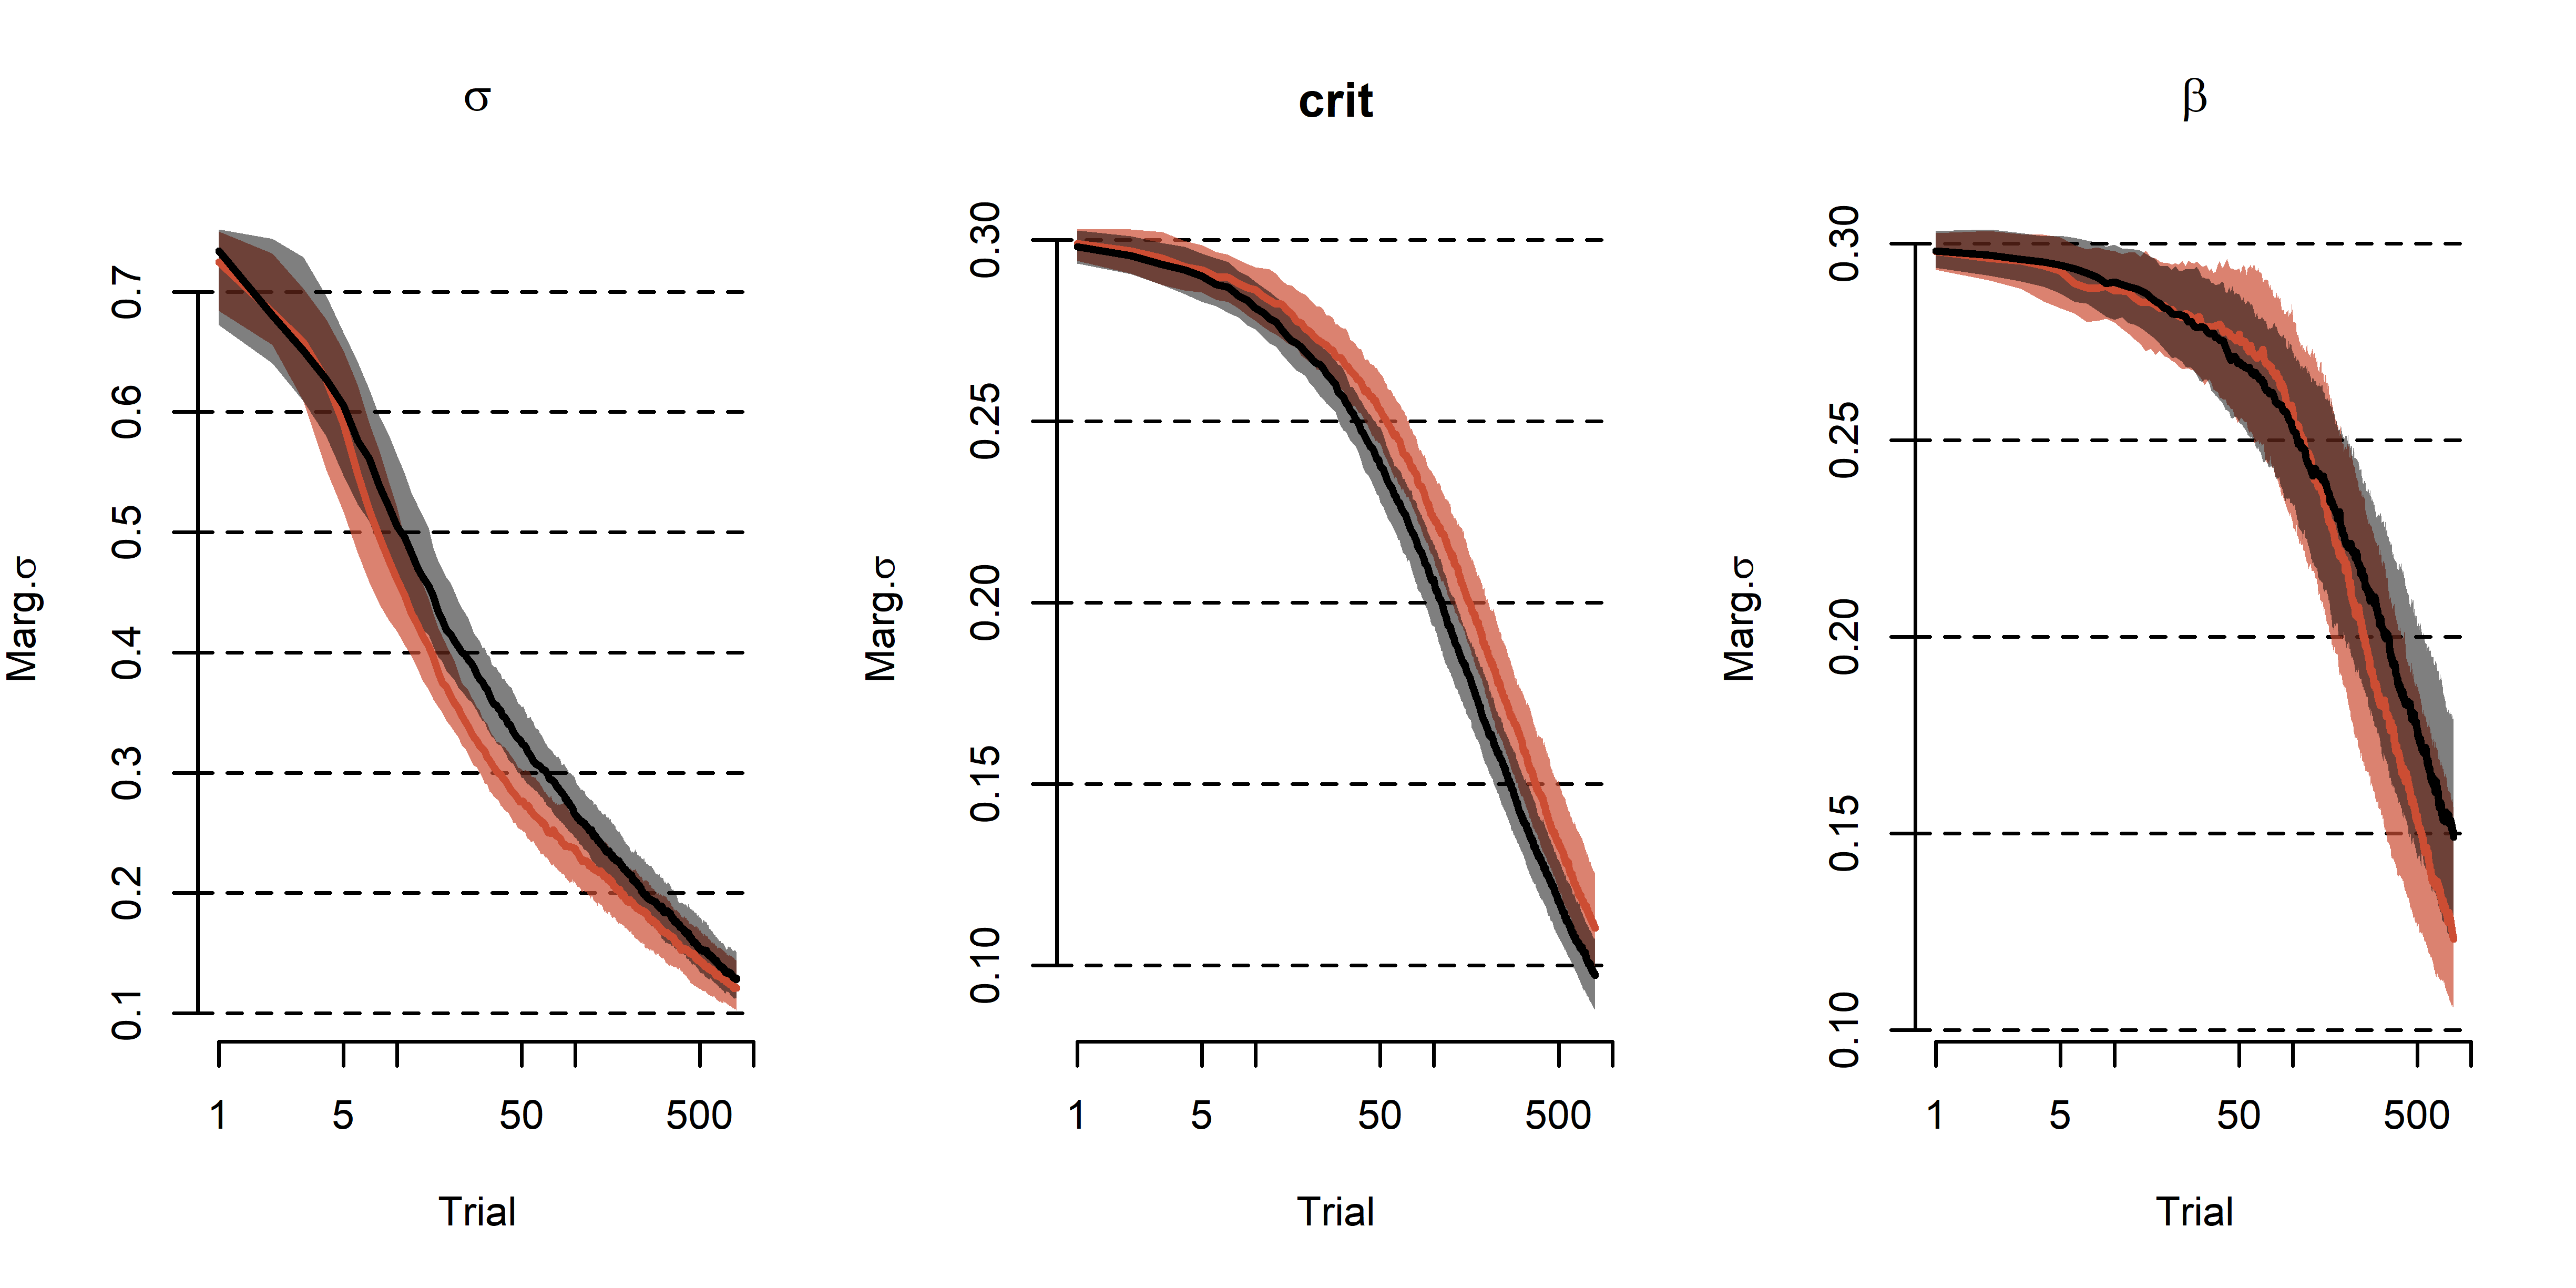
\includegraphics[scale=0.75, angle = 0]{simulation_YN_sensory_SD}
\caption{Procedure: Yes/No; sensory parameters. Trial-by-trial marginal standard deviations. Red: adaptive algorithm; black: random stimuli.}
\label{fig:simulation_YN_sensory_SD}
\end{figure}

\begin{figure}[H]
\centering
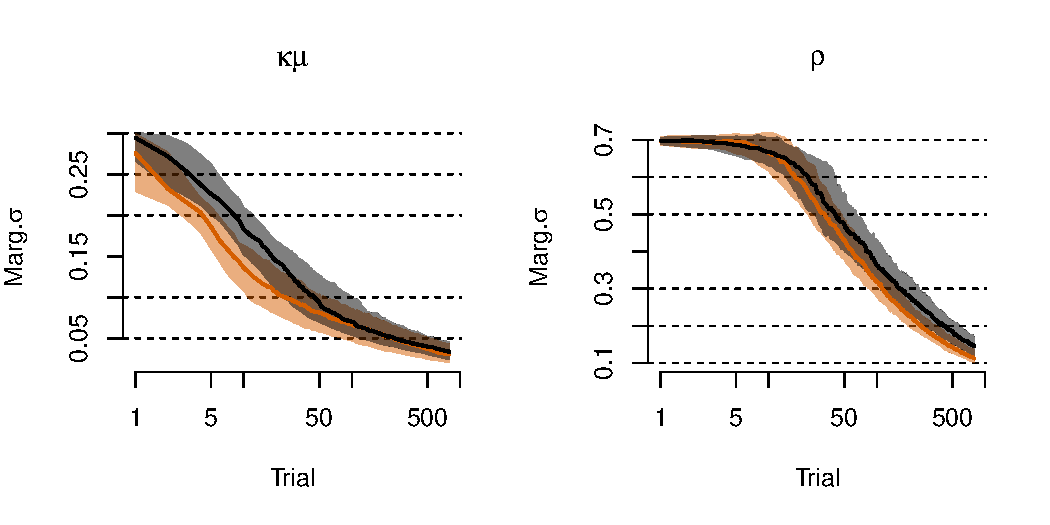
\includegraphics[scale=0.75, angle = 0]{simulation_YN_interaction_SD}
\caption{Procedure: Yes/No; interaction parameters. Trial-by-trial marginal standard deviations. Red: adaptive algorithm; black: random stimuli.}
\label{fig:simulation_YN_interaction_SD}
\end{figure}

\begin{figure}[H]
\centering
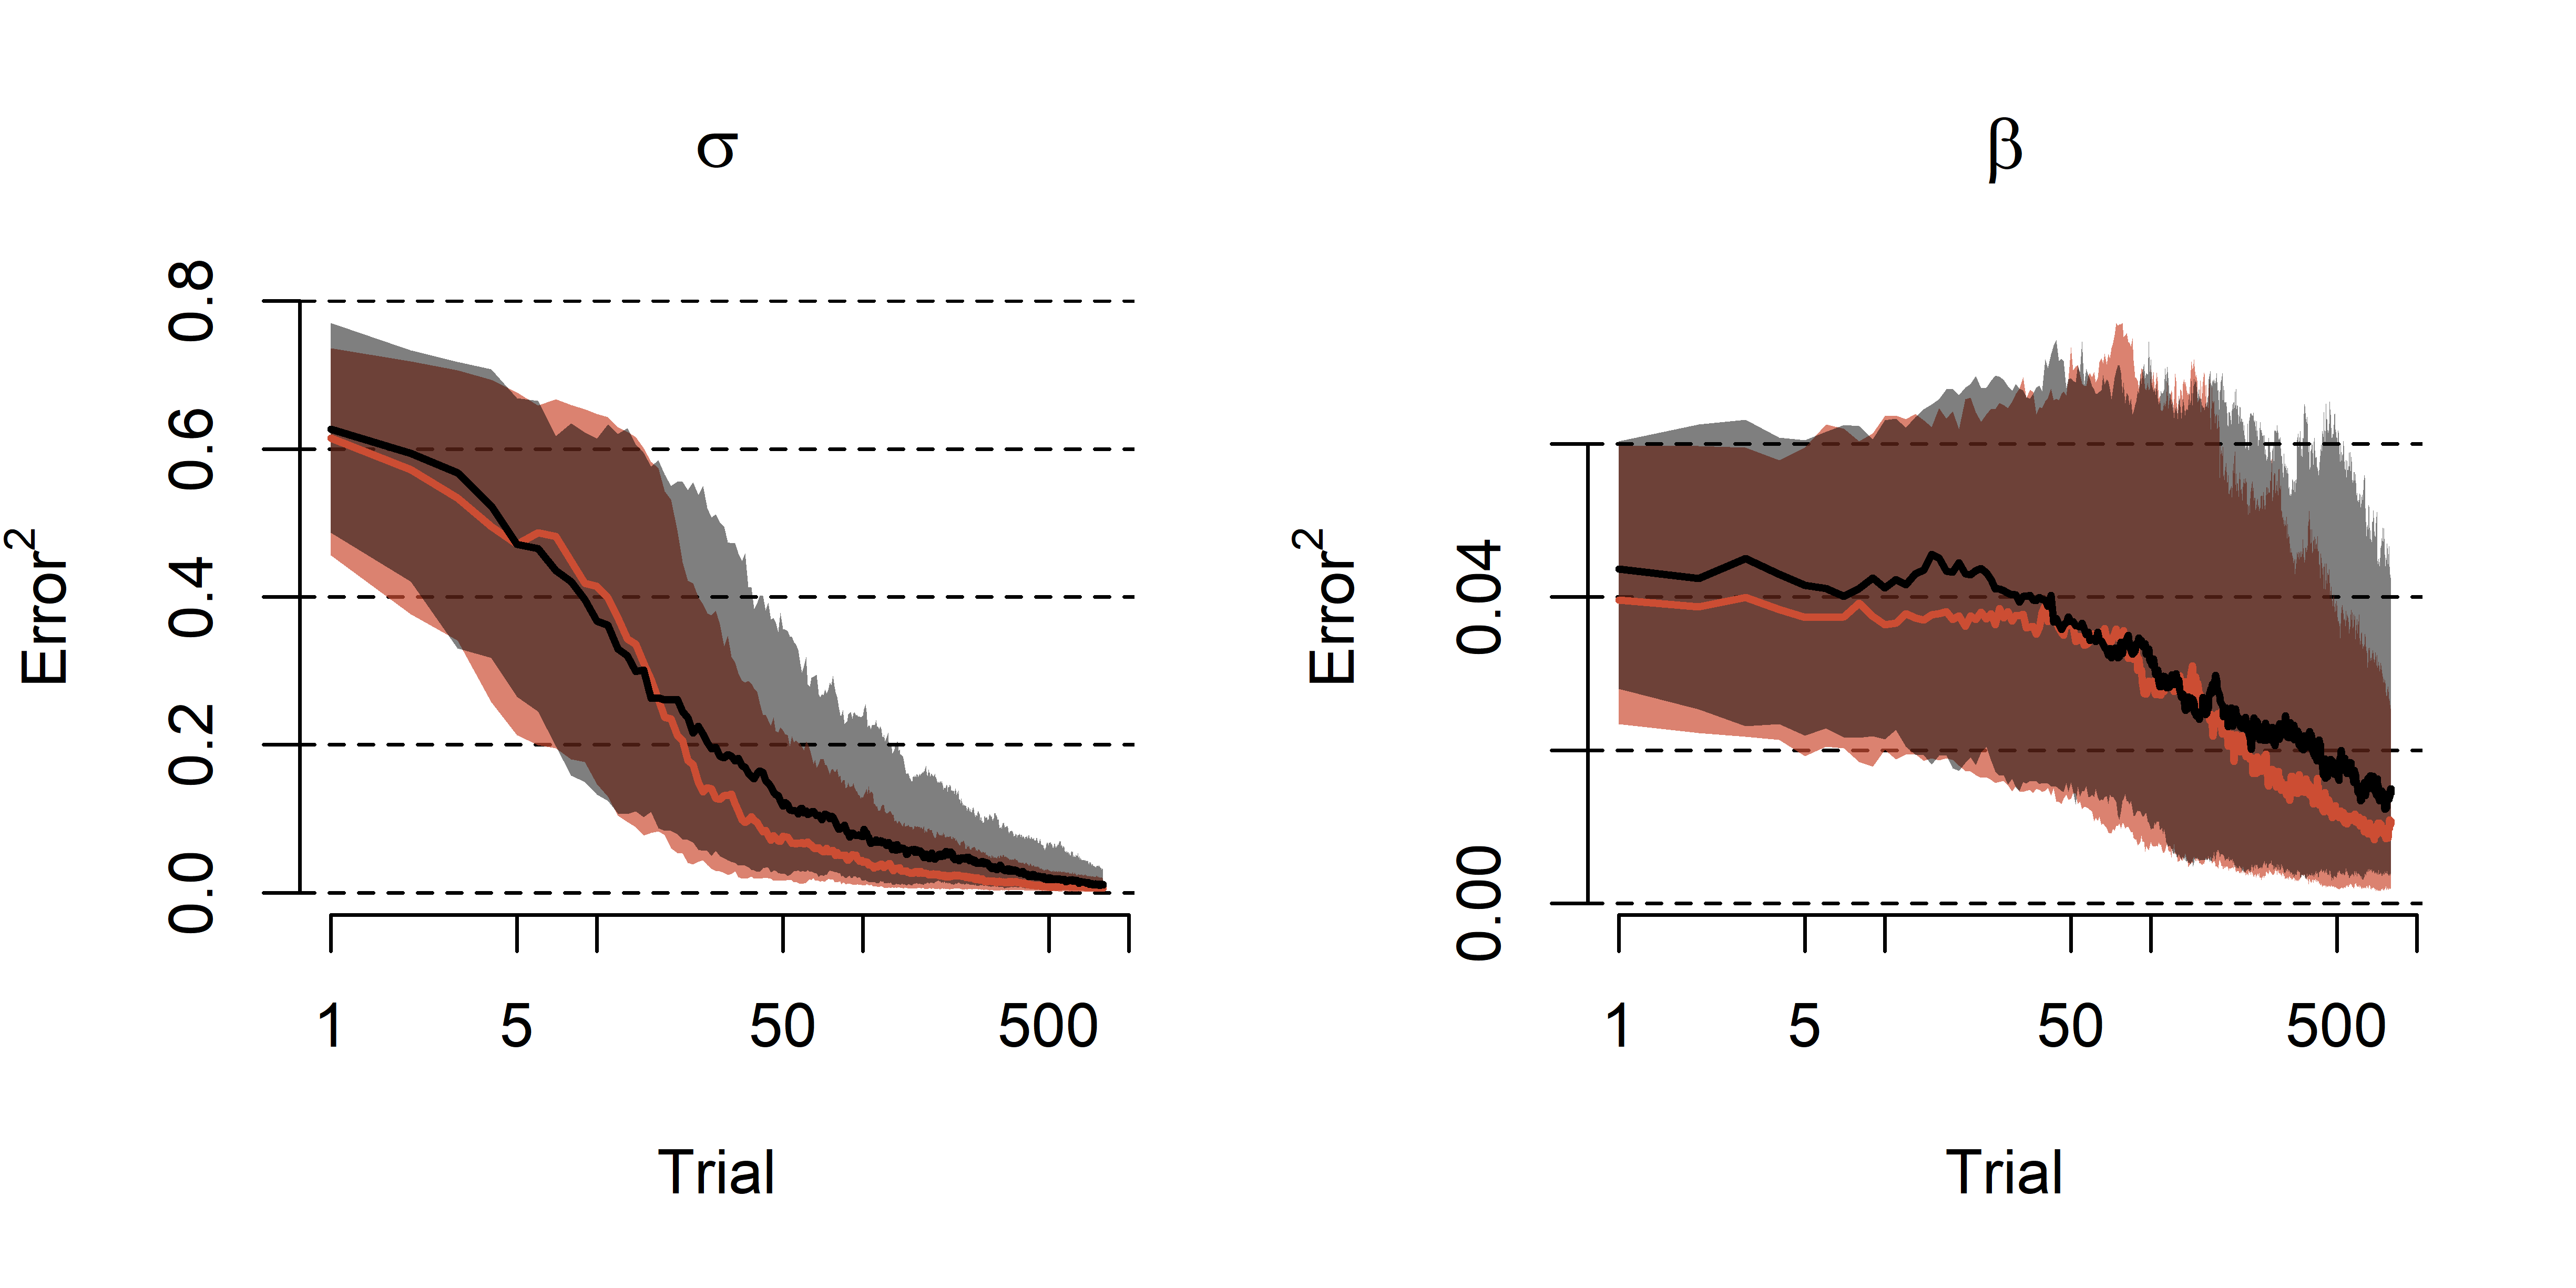
\includegraphics[scale=0.75, angle = 0]{simulation_AFC_sensory_sq_error}
\caption{Procedure: 2I-4AFC; sensory parameters. Trial-by-trial squared error between marginal means of the posterior distribution and generating parameters. Red: adaptive algorithm; black: random stimuli.}
\label{fig:simulation_AFC_sensory_sq_error}
\end{figure}

\begin{figure}[H]
\centering
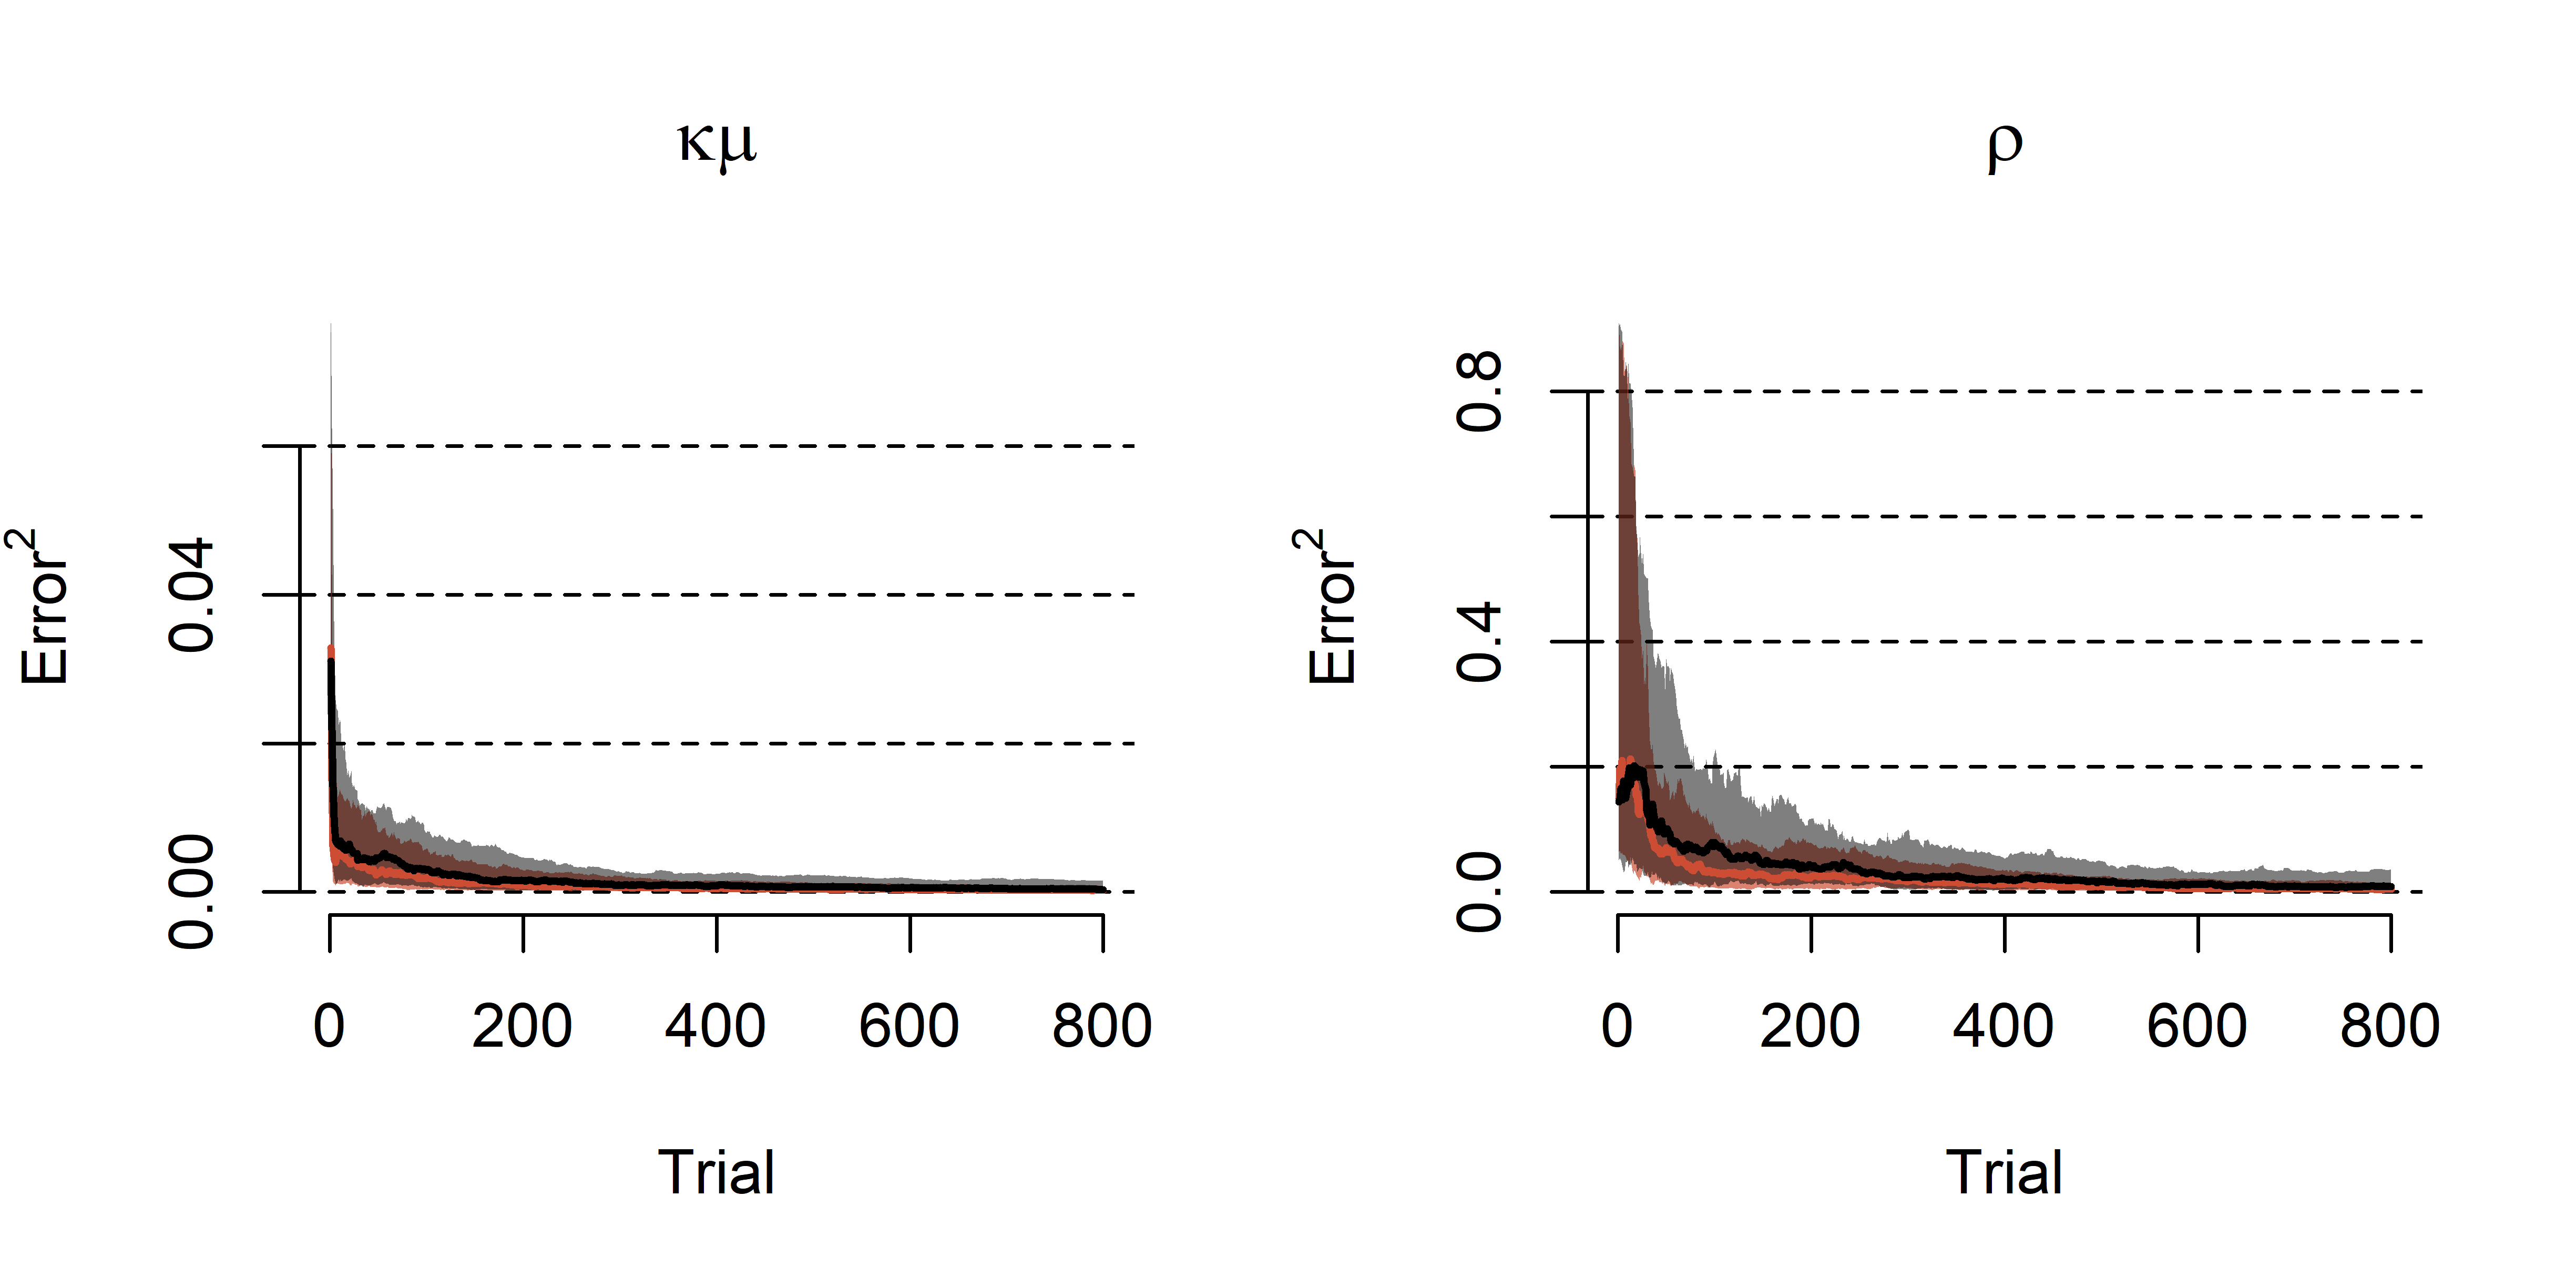
\includegraphics[scale=0.75, angle = 0]{simulation_AFC_interaction_sq_error}
\caption{Procedure: 2I-4AFC; interaction parameters. Trial-by-trial squared error between marginal means of the posterior distribution and generating parameters. Red: adaptive algorithm; black: random stimuli.}
\label{fig:simulation_AFC_interaction_sq_error}
\end{figure}

\begin{figure}[H]
\centering
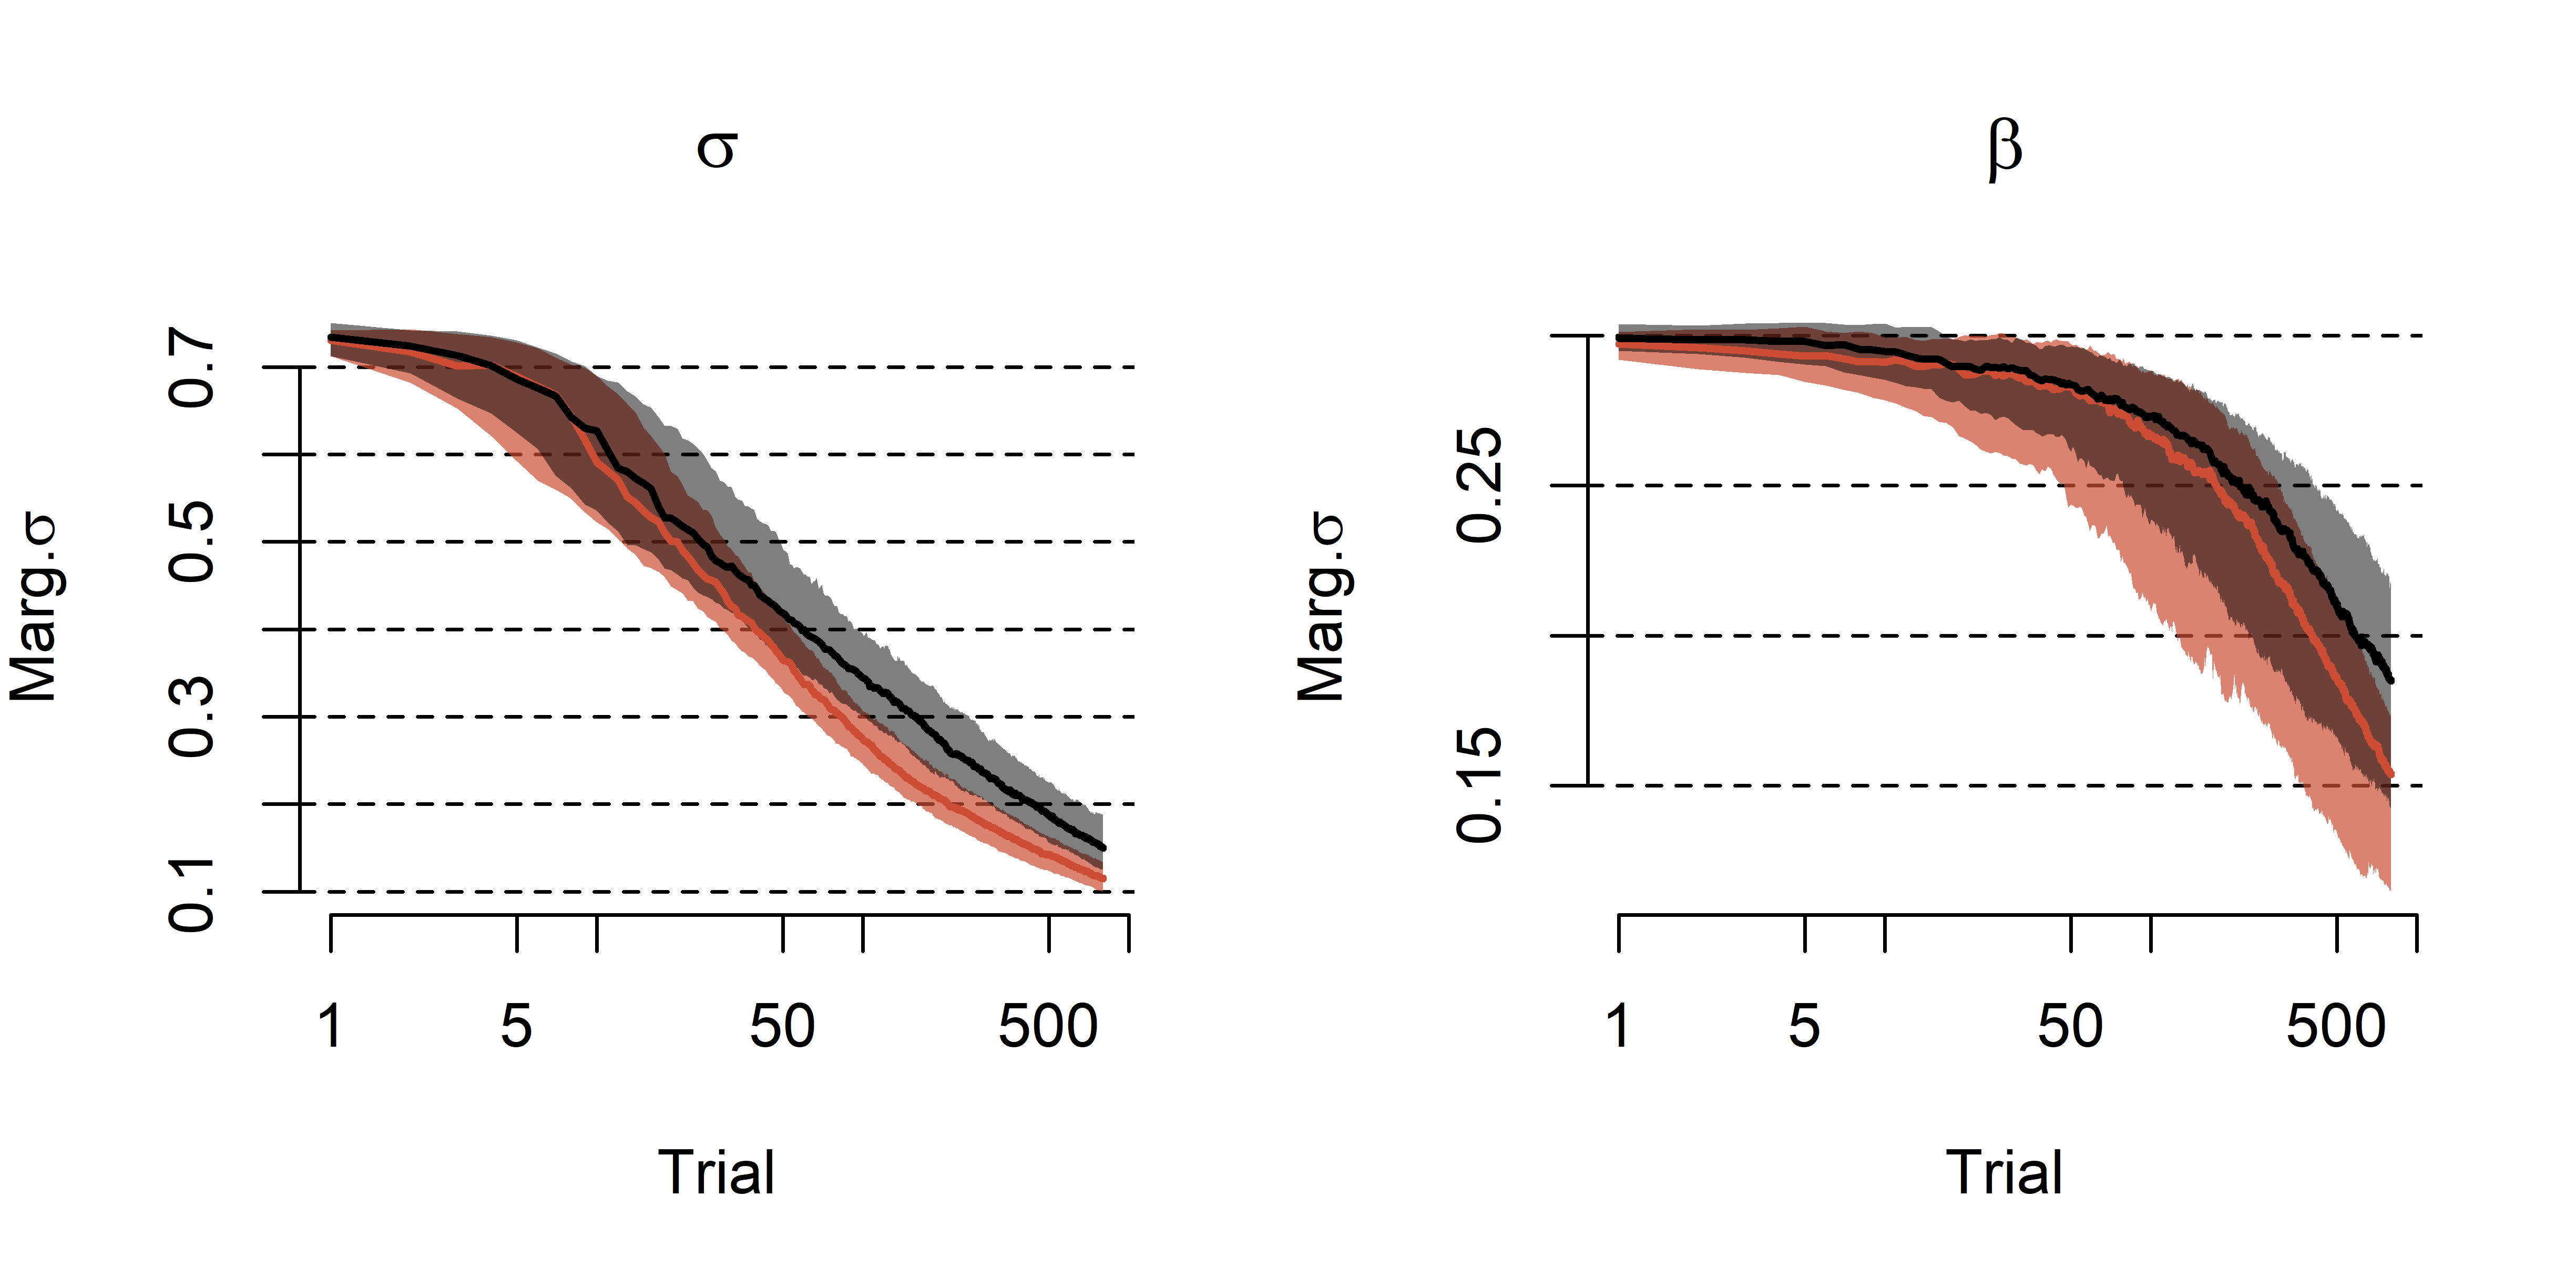
\includegraphics[scale=0.75, angle = 0]{simulation_AFC_sensory_SD}
\caption{Procedure: 2I-4AFC; sensory parameters. Trial-by-trial marginal standard deviations. Red: adaptive algorithm; black: random stimuli.}
\label{fig:simulation_AFC_sensory_SD}
\end{figure}

\begin{figure}[H]
\centering
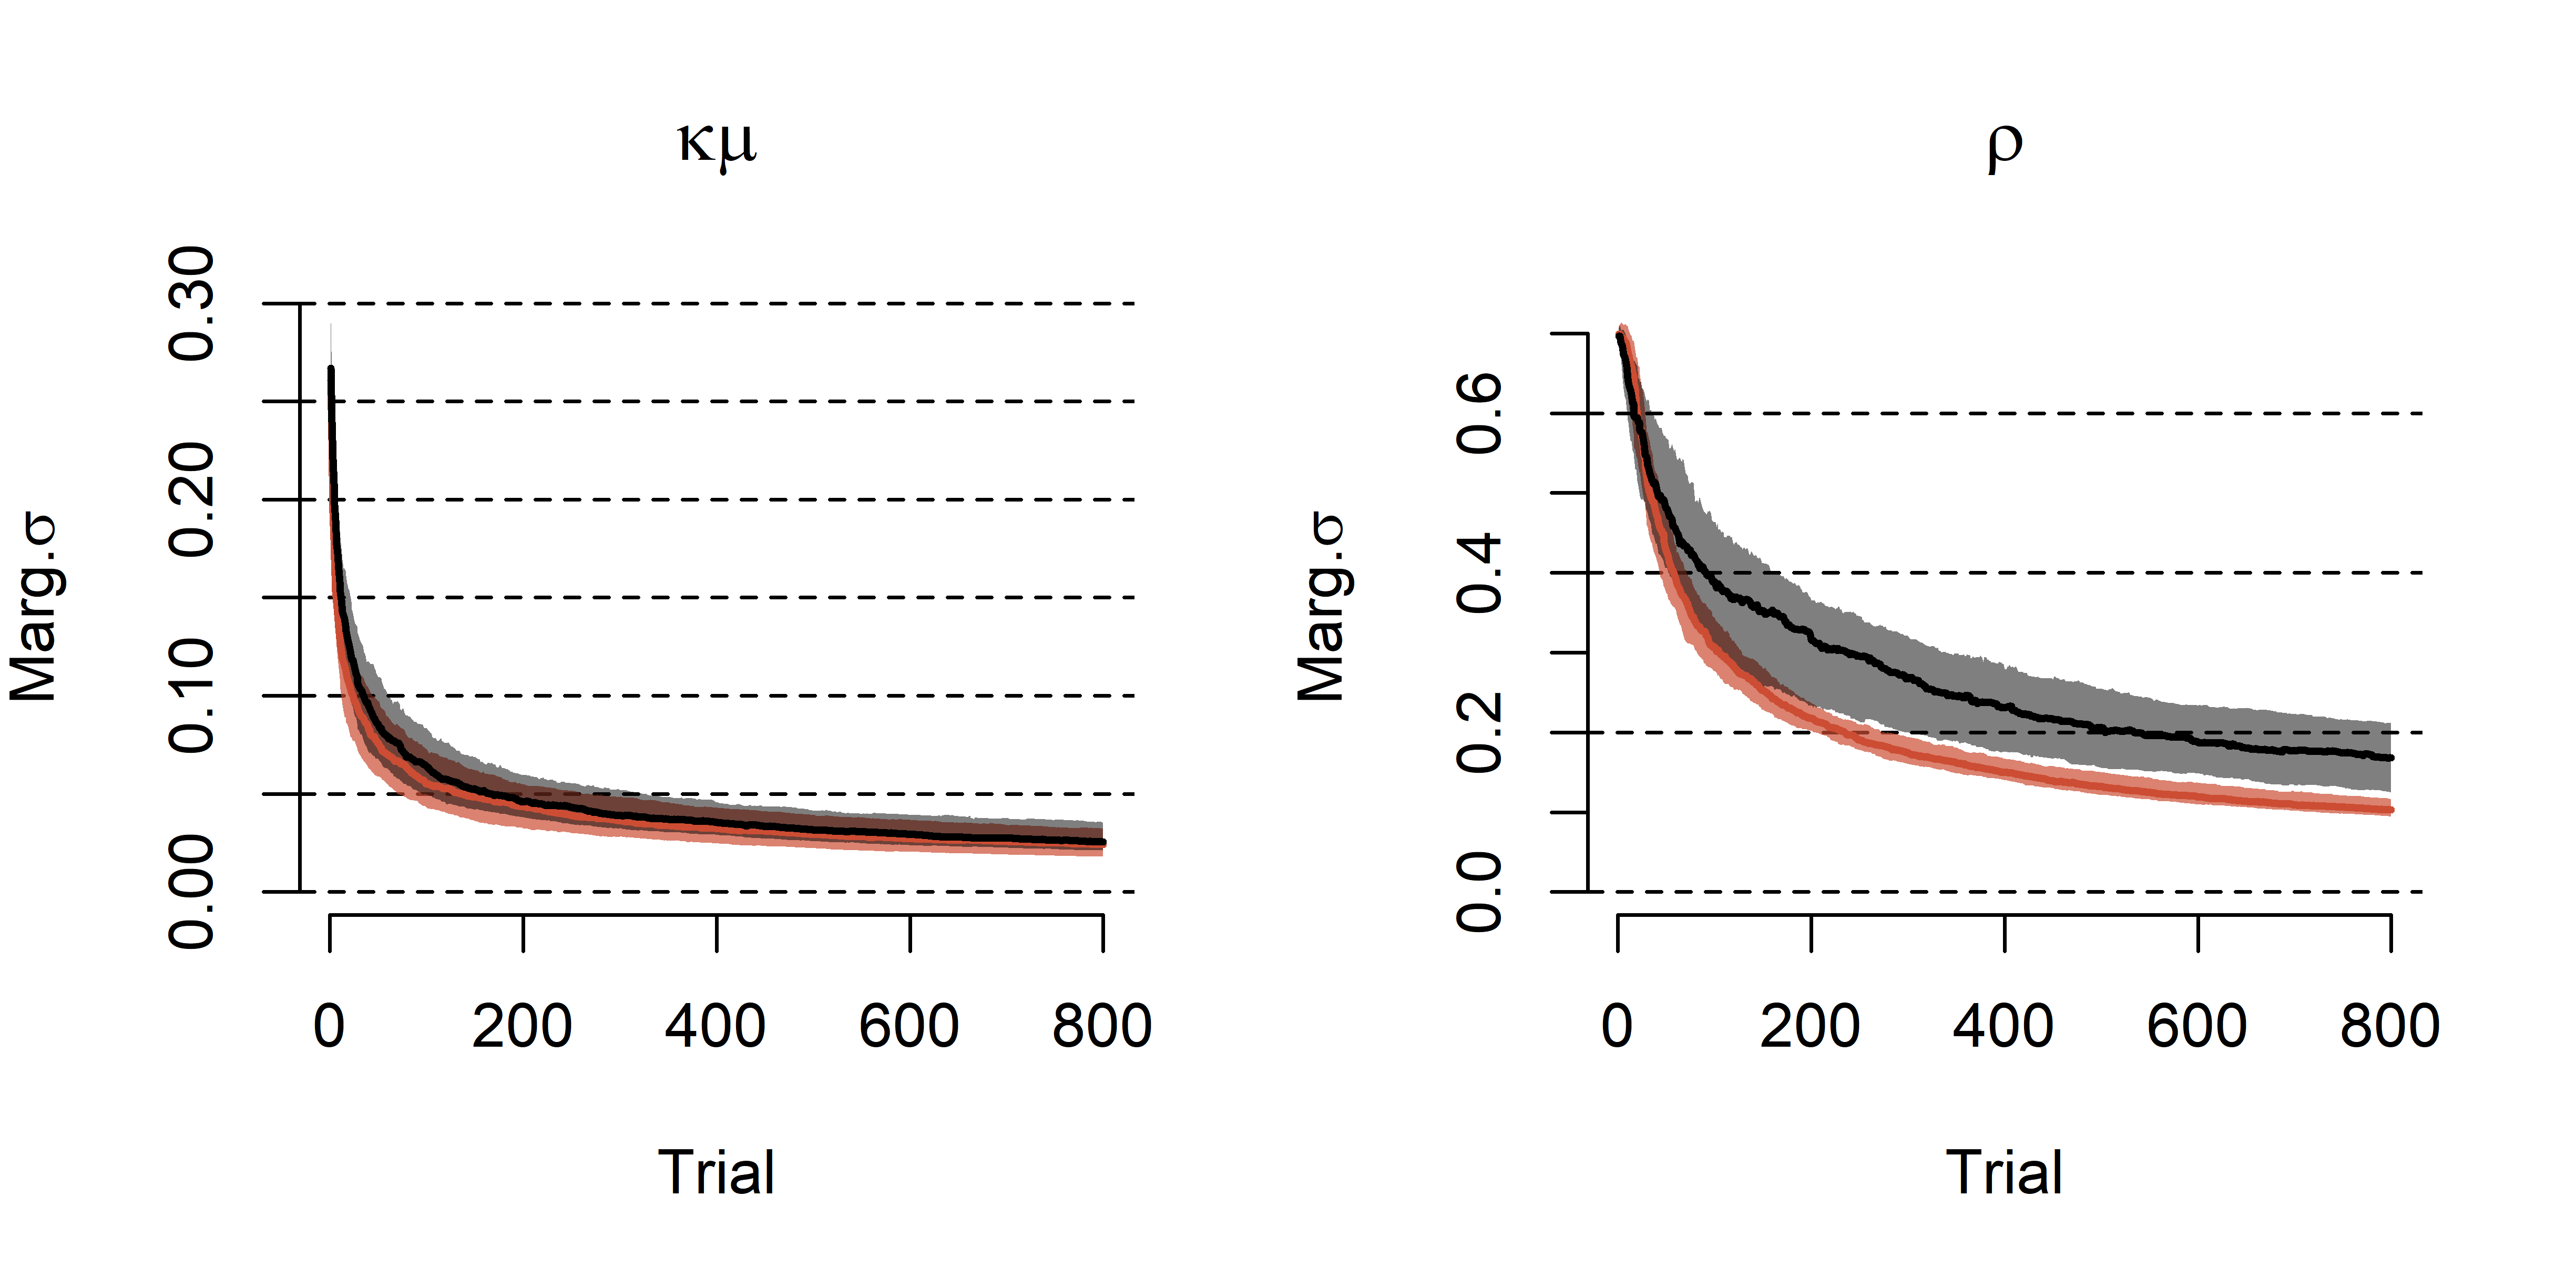
\includegraphics[scale=0.75, angle = 0]{simulation_AFC_interaction_SD}
\caption{Procedure: 2I-4AFC; interaction parameters. Trial-by-trial marginal standard deviations. Red: adaptive algorithm; black: random stimuli.}
\label{fig:simulation_AFC_interaction_SD}
\end{figure}

\paragraph{Hierarchical model}

A hierarchical model was fit to both the marginal standard deviations and squared errors at the last trial to get a more quantitative understanding of the differences at that point. This should be considered as a first-order approximation of a more complete model of performance. Why only the estimates at the last trial are presented is because for any simple model which breaks the performance down in two factors, namely the final values and the speed at which they were arrived at, only one of the factors needs to be known. This is because all of the algorithms start from the same values (the prior distribution) and are run for the same amount of time (800 trials). Of course some more sophisticated model, that would perform more complex decomposition of performance could be used, but the development of such algorithm is beyond the scope of this thesis. 

A common dummy coded linear model with Gaussian errors was used. The slopes, intercepts and standard deviations were pooled inside each condition, which means that e.g. all of the marginal standard deviations in the Yes/No condition with adaptively selected stimuli were given a common hyperprior. The models were fit using Stan, model code can be found online from \url{https://github.com/joanpaak/ERROR}.

Data was standardized before fitting ($y' = (y - \overline{y}) / \text{SD}(y) $). Parameter-specific $\beta'$ coefficients (slopes fit to standardized data) of the linear model are shown in Figures from \ref{fig:qs_YN_SD} to \ref{fig:qs_AFC_sq_error}. In all plots the thicker parts indicate 50\% and narrower lines 95\% equal-tailed intervals\footnote{\textit{Equal-tailed interval} (ETI) means the interval between some percentiles of the posterior distribution \citep[p. 342]{kruschke2015}, here for example the interval between 2.5\% and 97.5\% for the 95\% ETI.}. Positive values indicate better performance by the adaptive algorithm.

\begin{figure}[H]
\centering
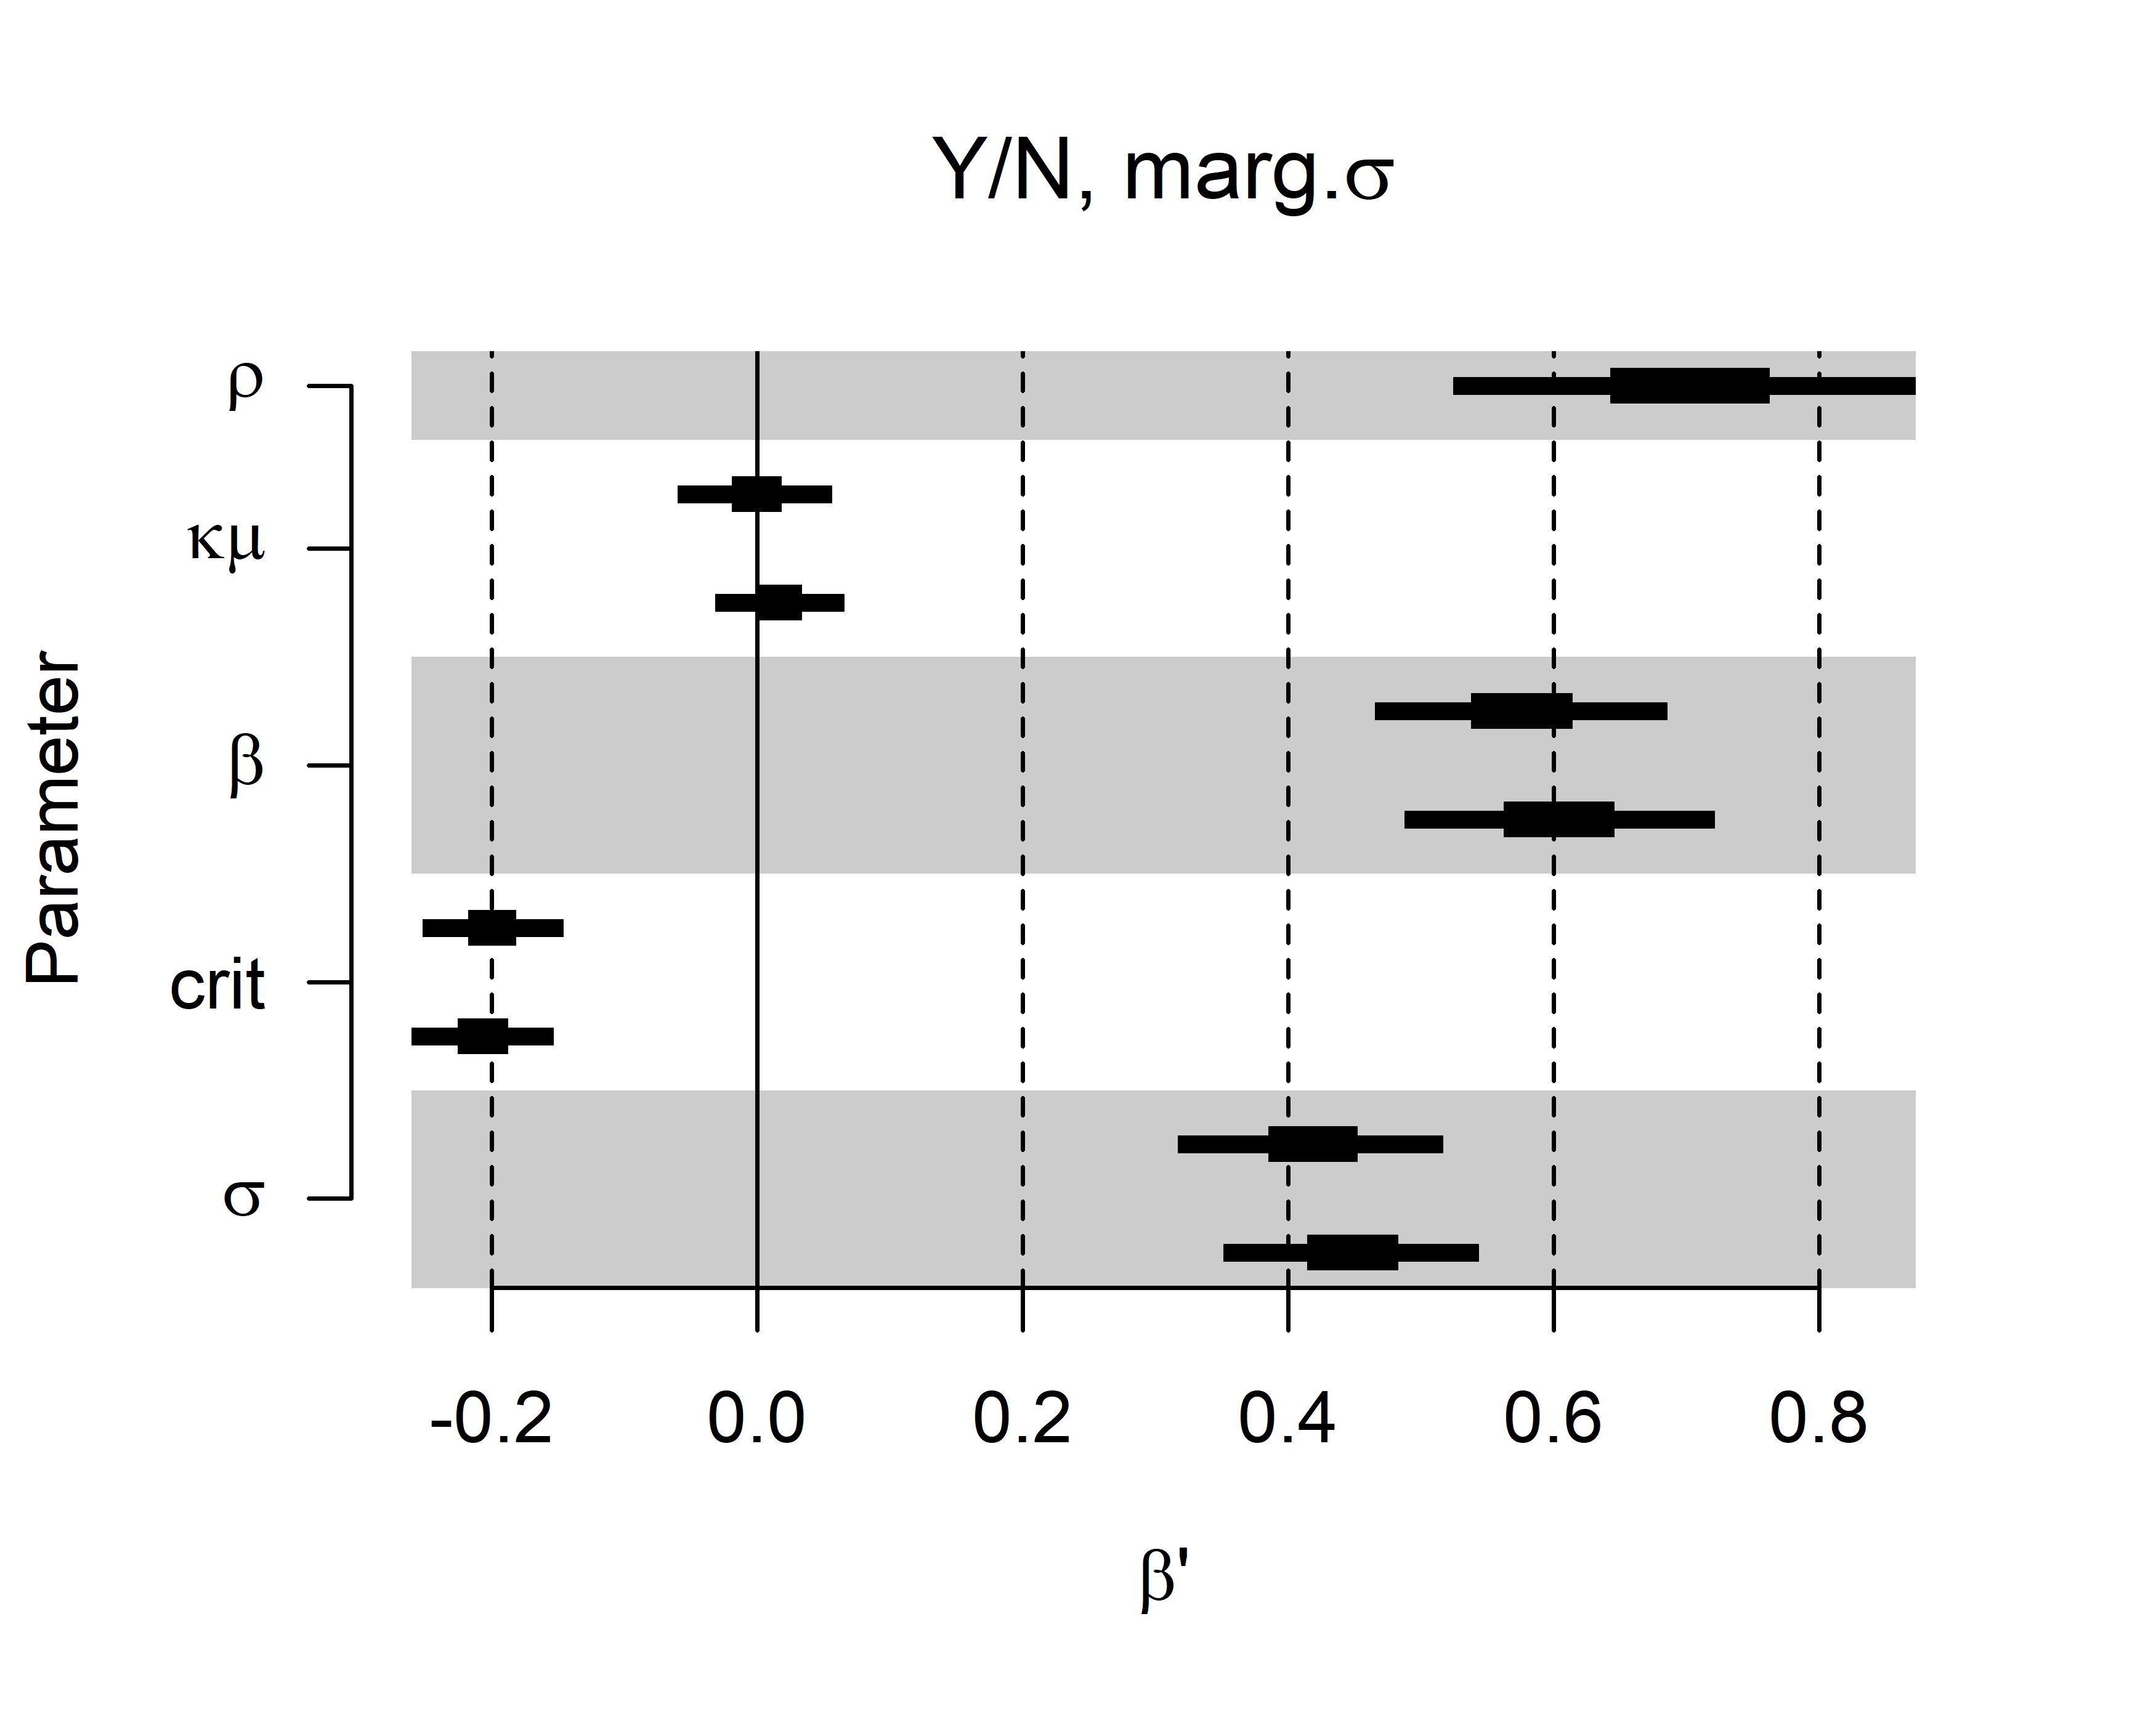
\includegraphics[scale=0.75]{qs_YN_SD}
\caption{Procedure: Yes/No. $\beta'$ coefficients for the difference between adaptive and random algorithms in marginal standard deviations.}
\label{fig:qs_YN_SD}
\end{figure} 

\begin{figure}[H]
\centering
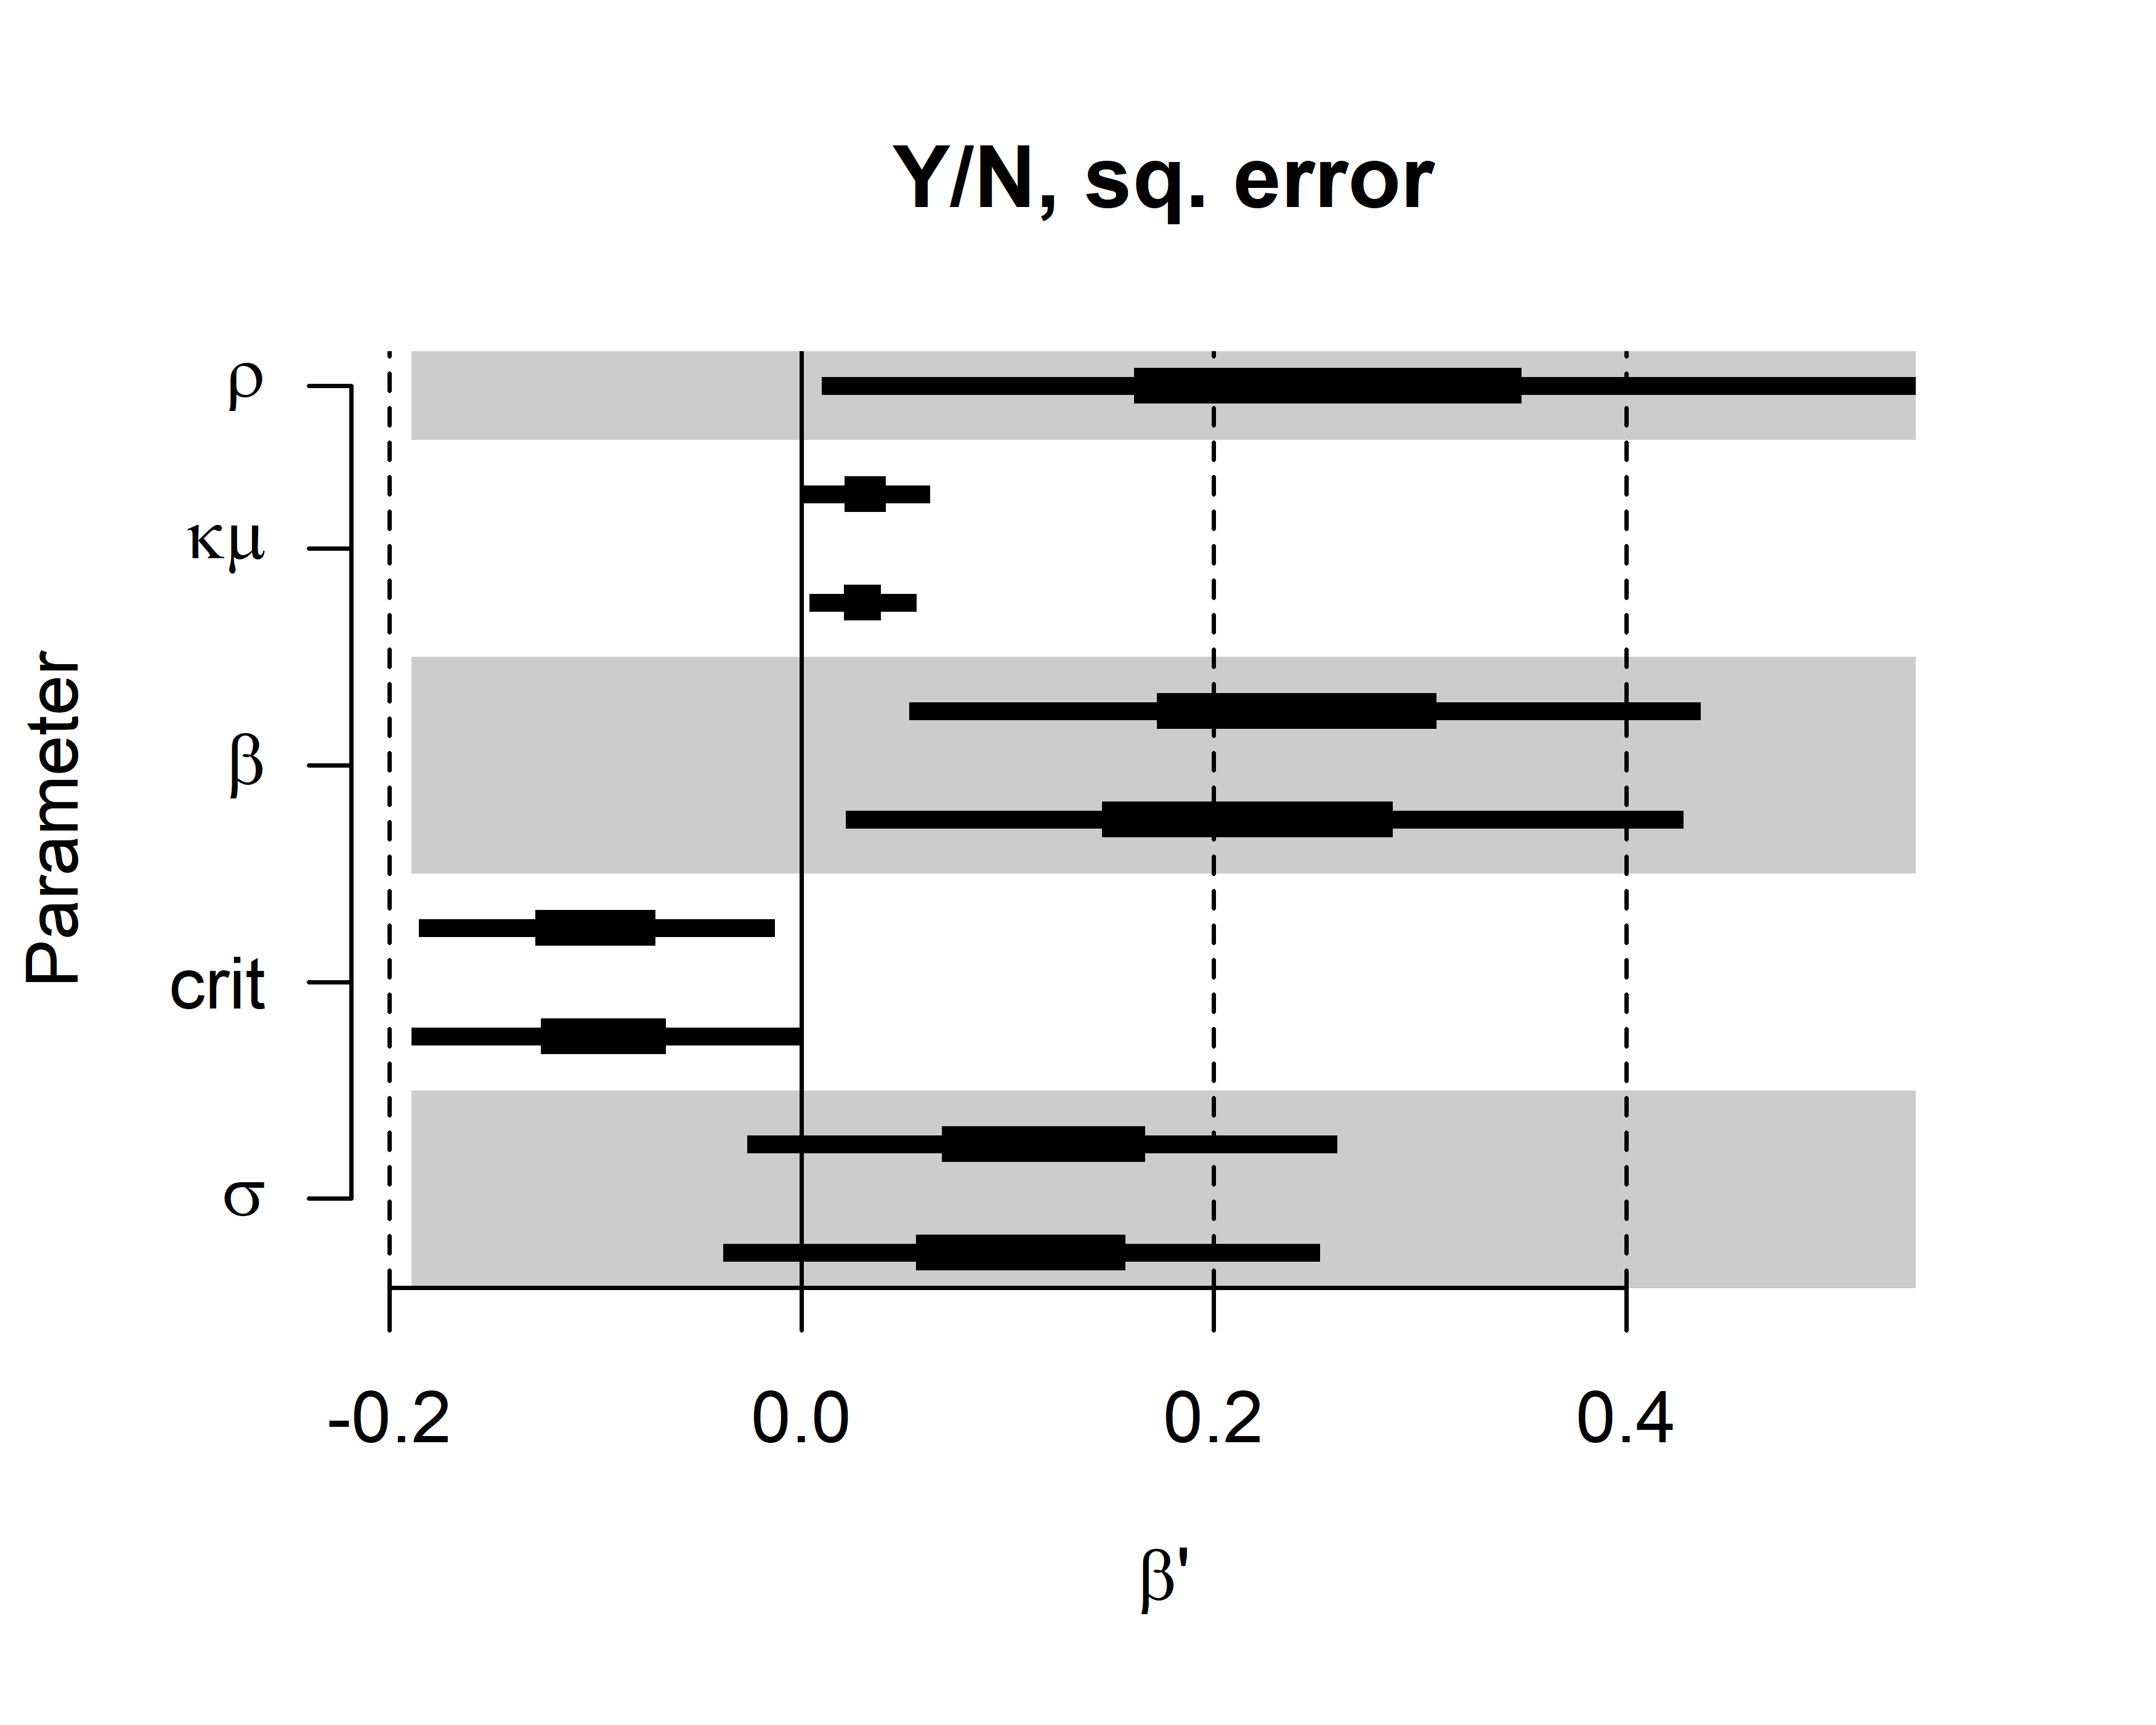
\includegraphics[scale=0.75]{qs_YN_sq_error}
\caption{Procedure: Yes/No. $\beta'$ coefficients for the difference between adaptive and random algorithms in squared errors between marginal means and generating parameters.}
\label{fig:qs_YN_sq_error}
\end{figure} 

\begin{figure}[H]
\centering
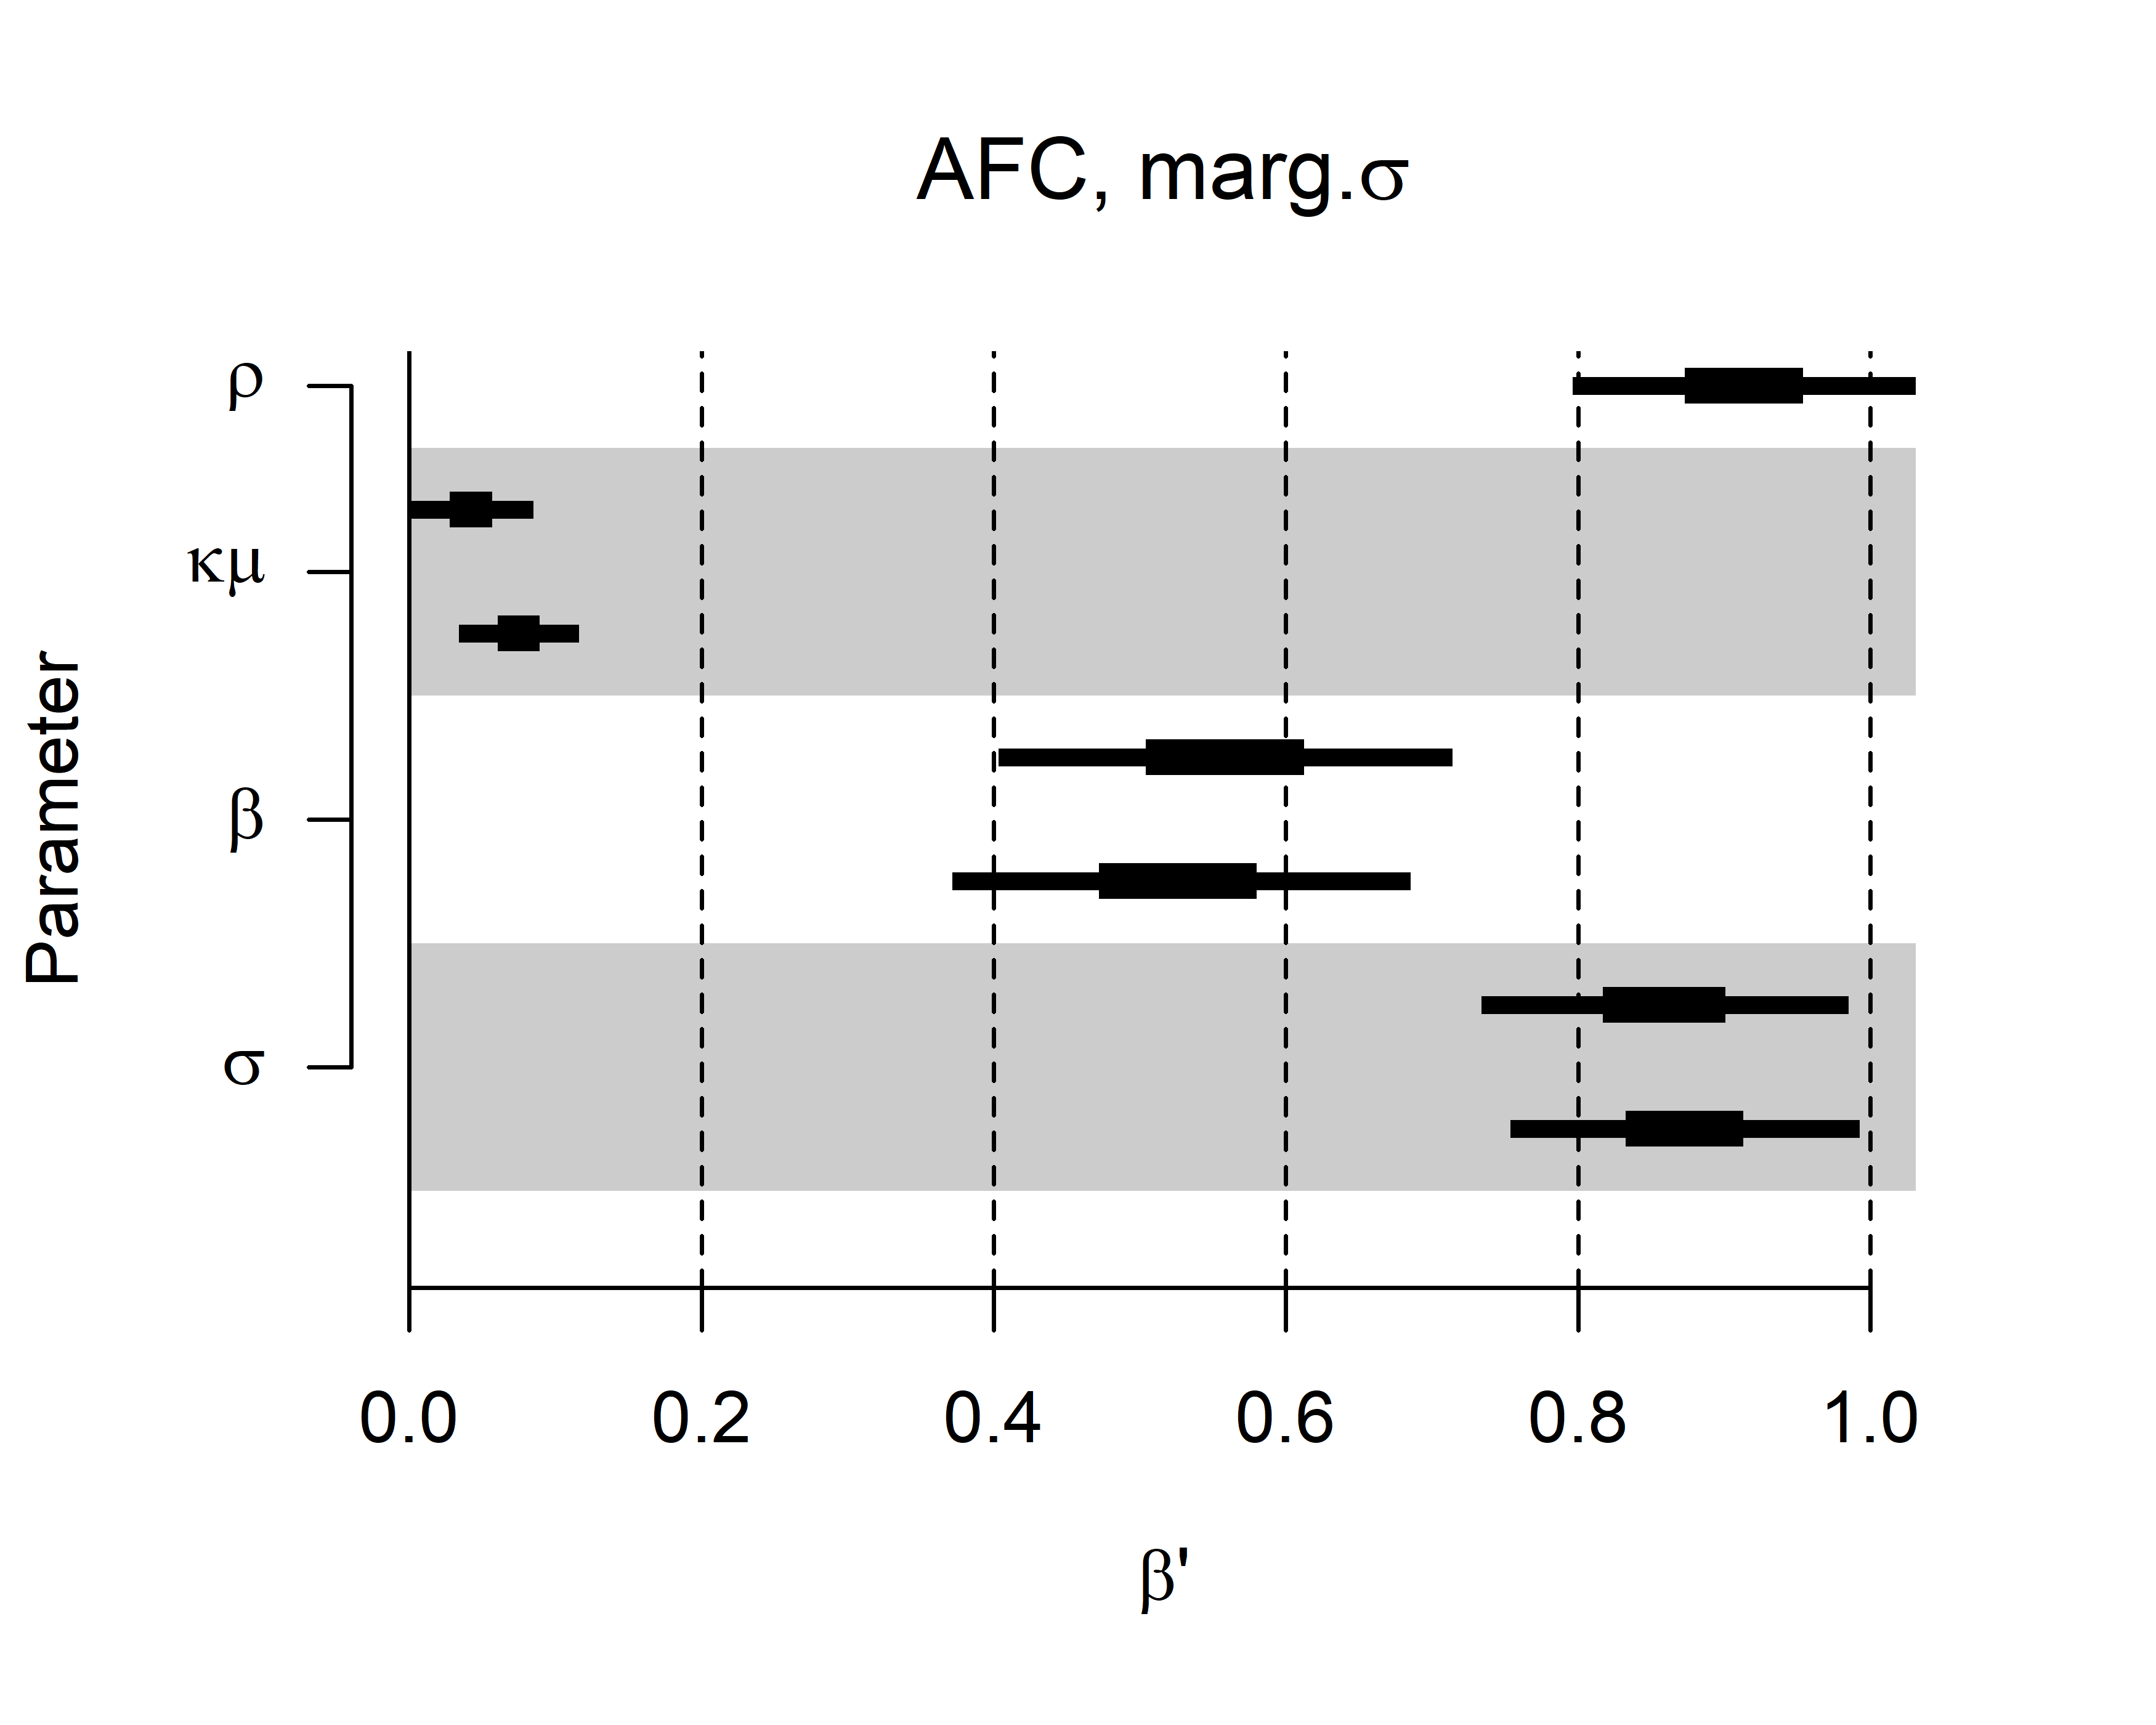
\includegraphics[scale=0.75]{qs_AFC_SD}
\caption{Procedure: 2I-4AFC. $\beta'$ coefficients for the difference between adaptive and random algorithms in marginal standard deviations.}
\label{fig:qs_AFC_SD}
\end{figure} 

\begin{figure}[H]
\centering
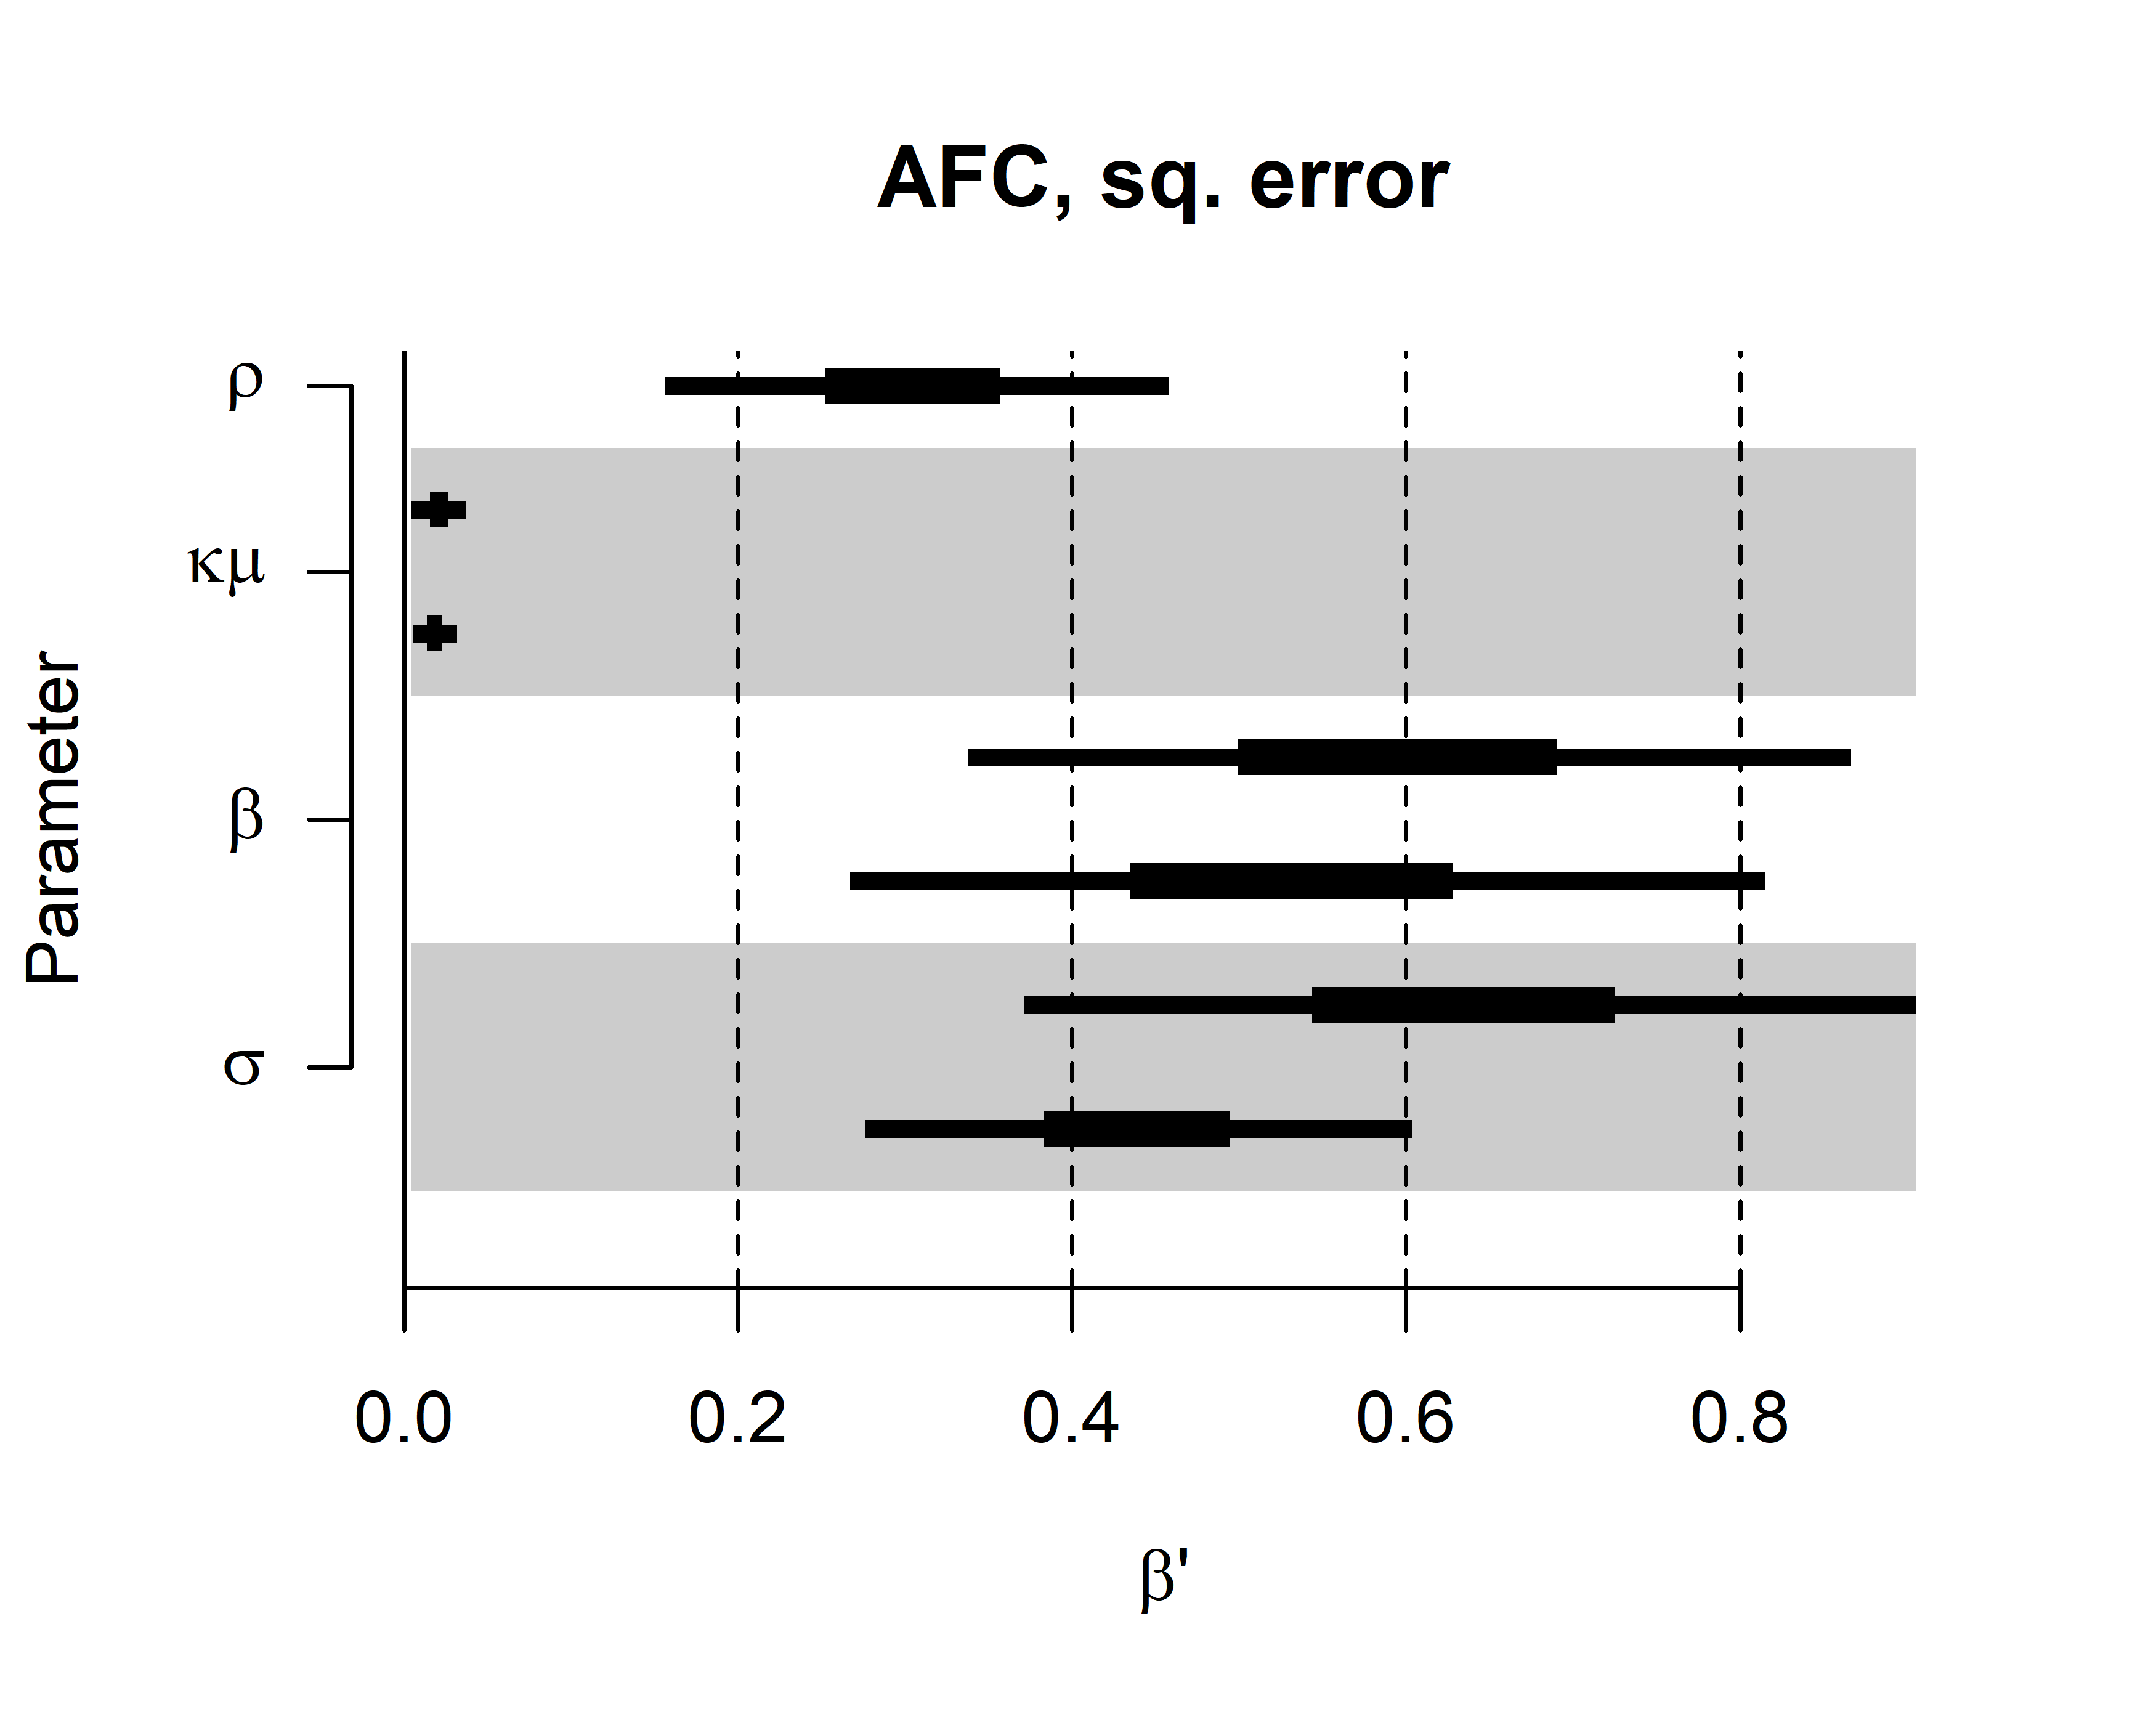
\includegraphics[scale=0.75]{qs_AFC_sq_error}
\caption{Procedure: 2I-4AFC. $\beta'$ coefficients for the difference between adaptive and random algorithms in squared errors between marginal means and generating parameters.}
\label{fig:qs_AFC_sq_error}
\end{figure} 

\subsection{Discussion}

\paragraph{Question 1: is the adaptive algorithm more efficient?}

Judging from Figures \ref{fig:qs_YN_SD} and \ref{fig:qs_AFC_SD}, by the time of 800 completed trials the adaptive algorithm has managed to reduce marginal standard deviations more for parameters $\sigma$, $\beta$ and $\rho$ in both conditions. Effect sizes range from around $0.4$ to almost $1.0$. However, as can be seen from Figures \ref{fig:simulation_YN_sensory_SD}, \ref{fig:simulation_YN_interaction_SD}, \ref{fig:simulation_AFC_sensory_SD} and \ref{fig:simulation_AFC_interaction_SD}, differences in raw scores are fairly modest, around 0.05 to 0.20.

There doesn't seem to be that much difference in $\kappa_{\mu}$ parameters, which is probably explained by the fact that, as can be seen from Figures \ref{fig:simulation_AFC_interaction_SD} and \ref{fig:simulation_YN_interaction_SD} the marginal standard deviations for these parameters reduce fairly quickly.

The most surprising result is that random sampling seems to be more effective in reducing uncertainty about the criteria (Figure \ref{fig:qs_YN_SD}). 

Similar pattern can be observed for the squared errors (Figures \ref{fig:qs_YN_sq_error} and \ref{fig:qs_AFC_sq_error}) but the differences are swamped by a lot more variability. 

\paragraph{Question 2: how well are generating parameters recovered?}

It seems that the majority of of improvement for most parameters happens before 400 trials. After that, information gain seems to slow down considerably.

The most problematic parameters would seem to be the $\beta$ parameters. This contrasts results in for example \cite{kontsevichtyler1999}, and could indicate that when in this more complex model inferences about the non-linearity of the $d'$ function become more uncertain. Note also that the variance of squared error in estimating the $\beta$ parameter increses somewhat during the first 100 trials (Figures \ref{fig:simulation_YN_sensory_sq_error} and \ref{fig:simulation_AFC_sensory_sq_error}, but the effect is more pronounced in the Yes/No condition), implying that for some simulations the posterior means drift further from the generating parameters. 

With regard to the interaction terms, squared errors and marginal standard deviations for the $\kappa_{\mu}$ parameters seem to approach zero fairly quickly, most of the improvements seems to have happened well before 100 trials, but the $\rho$ parameters seem more problematic (Figures \ref{fig:simulation_YN_interaction_sq_error}, \ref{fig:simulation_YN_interaction_SD}, \ref{fig:simulation_AFC_interaction_sq_error} and \ref{fig:simulation_AFC_interaction_SD}). Marginal standard deviations for the $\rho$s don't get, on average, much smaller than $.2$ which still implies a lot of uncertainty--keeping in mind that correlation coefficients are bound between $-1$ and $1$.

\clearpage
\bibliography{references}
\bibliographystyle{apacite}

\end{document}
